% !TEX root = ../main.tex
\section{Úroveň 2: Speciální Nelineární Rovnice 1. Řádu}
\label{sec:level2}

\subsection{Úvod do Úrovně 2}
\label{subsec:uvod-uroven-2}

Tato úroveň představuje systematický přechod od lineární k nelineární dynamice, otevírající cestu k modelování komplexních reálných systémů v kvantitativních vědách. Zatímco úroveň 1 poskytla kompletní fundament pro lineární a kvazilineární systémy, úroveň 2 rozšiřuje tento aparát na podstatně bohatší třídu nelineárních jevů.

\vspace{0.8\baselineskip}

\begin{principle}[Filozofie úrovně 2]
Úroveň 2 kombinuje rigorózní matematickou analýzu s hlubokým důrazem na kvalitativní chování řešení. Neusilujeme pouze o nalezení explicitního řešení, ale o pochopení strukturálních vlastností nelineárních systémů a jejich implikací pro kvantitativní modelování.
\end{principle}

\vspace{0.8\baselineskip}

\subsubsection*{Organizace a cíle úrovně}

Úroveň 2 je strukturována do pěti klíčových tříd nelineárních ODE 1. řádu, z nichž každá reprezentuje specifický typ nelinearity a vyžaduje specializovaný matematický přístup:

\begin{itemize}
\item \textbf{Bernoulliho rovnice} - nelinearita ve formě mocniny a její transformace na lineární tvar
\item \textbf{Riccatiho rovnice} - kvadratická nelinearita s aplikacemi v optimalizaci a řízení
\item \textbf{Clairautovy rovnice} - singulární řešení a teorie obálek
\item \textbf{Lagrangeovy rovnice} - parametrické řešení a zobecnění předchozího případu
\item \textbf{Abelovy rovnice} - kubická nelinearita a její speciální integrabilní případy
\end{itemize}

\vspace{0.8\baselineskip}

\subsubsection*{Kvantitativní význam}

Pro kvantitativního experta představují nelineární rovnice 1. řádu nezbytný nástroj pro:

\begin{itemize}
\item Modelování nelineárních růstových procesů v ekonomii a financích
\item Analýzu stability komplexních systémů s více rovnovážnými stavy
\item Studium bifurkací a přechodů mezi režimy chování
\item Přípravu na pokročilé nelineární modely včetně systémů vyšších řádů
\end{itemize}

\vspace{0.8\baselineskip}

\begin{example}[Motivační příklad z ekonomického modelování]
Uvažujme model technologické difuze s nelineární saturační efektem:
\[
\frac{dA}{dt} = rA\left(1 - \frac{A}{K}\right) - \alpha A^2
\]
Tato Bernoulliho rovnice s kvadratickým členem popisuje kompetitivní dynamiku v adaptaci nových technologií, kde dodatečný člen reprezentuje konkurenční tlaky na trhu.
\end{example}

\vspace{0.8\baselineskip}

\subsubsection*{Metodologický přístup}

Každý typ nelineární rovnice bude prezentován prostřednictvím kompletní teoretické analýzy, systematické řešicí metodologie, hierarchicky uspořádaných příkladů a bezprostředních aplikací v kvantitativních vědách. Důraz je kladen na porozumění transformacím, které umožňují redukci složitých nelineárních problémů na řešitelné podoby.

Tato úroveň nejenže rozšiřuje technický instrumentář, ale také kultivuje matematickou intuici pro práci s nelineárními systémy, což je nezbytná kompetence pro moderní kvantitativní výzkum.
\end{example}


\subsection{Bernoulliho Diferenciální Rovnice}
\label{subsec:bernoulliho-rovnice}

\subsubsection{Teoretický Fundament Bernoulliho Rovnic}
\label{subsubsec:teoreticky-fundament-bernoulli}

\begin{historical}[Jacob Bernoulli a historický kontext]
Jacob Bernoulli (1655-1705) zavedl tento typ rovnice při studiu problémů mechaniky a populační dynamiky. Jeho práce položila základy pro systematické studium nelineárních diferenciálních rovnic a jejich transformací na lineární tvary.
\end{historical}

\vspace{0.8\baselineskip}

\begin{definition}[Bernoulliho diferenciální rovnice]
\label{def:bernoulliho-rovnice}
Rovnice tvaru
\[
\frac{dy}{dx} + p(x)y = q(x)y^n
\]
kde $p(x)$ a $q(x)$ jsou spojité funkce na intervalu $I \subseteq \mathbb{R}$ a $n \in \mathbb{R}$, $n \neq 0, 1$, se nazývá \emph{Bernoulliho diferenciální rovnice}.
\end{definition}

\vspace{0.6\baselineskip}

\begin{remark}[Speciální případy a redukce]
\label{rem:specialni-pripady}
\begin{itemize}
\item Pro $n = 0$: Rovnice se redukuje na lineární nehomogenní rovnici
\item Pro $n = 1$: Rovnice se redukuje na lineární homogenní rovnici
\item Pro $n \neq 0, 1$: Jedná se o vlastní nelineární Bernoulliho rovnici
\end{itemize}
\end{remark}

\vspace{0.8\baselineskip}

\subsubsection{Transformace na Lineární Rovnici}
\label{subsubsec:transformace-linearni}

\begin{theorem}[Transformace Bernoulliho rovnice]
\label{th:transformace-bernoulli}
Nechť $y(x)$ je řešení Bernoulliho rovnice $\frac{dy}{dx} + p(x)y = q(x)y^n$ s $n \neq 0, 1$. Potom substituce
\[
v = y^{1-n}
\]
transformuje Bernoulliho rovnici na lineární rovnici
\[
\frac{dv}{dx} + (1-n)p(x)v = (1-n)q(x)
\]
\end{theorem}

\vspace{0.6\baselineskip}

\begin{proof}[Kompletní odvození transformace]
\label{proof:transformace-odvozeni}
Začneme s Bernoulliho rovnicí:
\[
\frac{dy}{dx} + p(x)y = q(x)y^n
\]

Zavedeme substituci $v = y^{1-n}$. Derivujeme podle $x$:
\[
\frac{dv}{dx} = \frac{d}{dx}(y^{1-n}) = (1-n)y^{-n}\frac{dy}{dx}
\]

Vyjádříme $\frac{dy}{dx}$:
\[
\frac{dy}{dx} = \frac{y^n}{1-n}\frac{dv}{dx}
\]

Dosadíme do původní rovnice:
\[
\frac{y^n}{1-n}\frac{dv}{dx} + p(x)y = q(x)y^n
\]

Vydělíme celou rovnici $y^n$ (za předpokladu $y \neq 0$):
\[
\frac{1}{1-n}\frac{dv}{dx} + p(x)y^{1-n} = q(x)
\]

Substituujeme $v = y^{1-n}$:
\[
\frac{1}{1-n}\frac{dv}{dx} + p(x)v = q(x)
\]

Vynásobíme $(1-n)$:
\[
\frac{dv}{dx} + (1-n)p(x)v = (1-n)q(x)
\]

Tím jsme získali lineární rovnici pro $v(x)$.
\end{proof}

\vspace{0.8\baselineskip}

\begin{method}[Systematická metodologie řešení]
\label{met:systematicka-metodologie}
\begin{enumerate}
\item \textbf{Krok 1: Identifikace parametrů}
\begin{itemize}
\item Určete $p(x)$, $q(x)$ a $n$
\item Analyzujte definiční obory funkcí $p(x)$, $q(x)$
\item Identifikujte možné singularitní body
\end{itemize}

\item \textbf{Krok 2: Transformace}
\begin{itemize}
\item Proveďte substituci $v = y^{1-n}$
\item Ověřte platnost transformace ($y \neq 0$)
\item Zapište transformovanou lineární rovnici
\end{itemize}

\item \textbf{Krok 3: Řešení lineární rovnice}
\begin{itemize}
\item Určete integrační faktor $\mu(x) = e^{\int (1-n)p(x)dx}$
\item Nalezněte obecné řešení $v(x)$
\item Ověřte správnost řešení derivací
\end{itemize}

\item \textbf{Krok 4: Zpětná transformace}
\begin{itemize}
\item Proveďte inverzní substituci $y = v^{1/(1-n)}$
\item Analyzujte definiční obor výsledného řešení
\item Ověřte řešení dosazením do původní rovnice
\end{itemize}
\end{enumerate}
\end{method}

\vspace{0.8\baselineskip}

\begin{example}[Kompletní ilustrace transformace]
\label{ex:kompletni-transformace}
Řešte rovnici: $\frac{dy}{dx} + 2xy = x^3y^3$

\textbf{Řešení}:
\begin{enumerate}
\item \textbf{Identifikace}: $p(x) = 2x$, $q(x) = x^3$, $n = 3$
\item \textbf{Transformace}: $v = y^{1-3} = y^{-2}$, tedy $y = v^{-1/2}$
\item \textbf{Derivace}: $\frac{dv}{dx} = -2y^{-3}\frac{dy}{dx}$
\item \textbf{Dosazení}: $-2y^{-3}\frac{dy}{dx} + (1-3)(2x)v = (1-3)x^3$
\item \textbf{Zjednodušení}: $\frac{dv}{dx} - 4xv = -2x^3$
\item \textbf{Integrační faktor}: $\mu(x) = e^{\int -4x dx} = e^{-2x^2}$
\item \textbf{Řešení pro $v$}: $v(x) = e^{2x^2}\left(\int -2x^3 e^{-2x^2} dx + C\right)$
\item \textbf{Výpočet integrálu}: $\int -2x^3 e^{-2x^2} dx = \frac{1}{2}(x^2 + \frac{1}{2})e^{-2x^2}$
\item \textbf{Výsledek}: $v(x) = \frac{1}{2}x^2 + \frac{1}{4} + Ce^{2x^2}$
\item \textbf{Zpětná transformace}: $y(x) = \left(\frac{1}{2}x^2 + \frac{1}{4} + Ce^{2x^2}\right)^{-1/2}$
\end{enumerate}
\end{example}

\vspace{0.8\baselineskip}

\begin{transition}
V další části prozkoumáme analýzu singularit, geometrickou interpretaci a systematickou klasifikaci různých typů Bernoulliho rovnic.
\end{transition}

\subsubsection{Analýza Singularit a Speciálních Případů}
\label{subsubsec:analyza-singularit}

\begin{analysis}[Singulární chování Bernoulliho rovnic]
\label{ana:singularni-chovani}
Bernoulliho rovnice vykazuje několik typů singulárního chování, které vyžadují speciální pozornost:

\begin{itemize}
\item \textbf{Nulové řešení}: Pro $n > 0$ je $y = 0$ řešením rovnice
\item \textbf{Singularity transformace}: Body kde $y = 0$ pro $n > 1$ nebo $y \to \infty$ pro $n < 1$
\item \textbf{Nedefinované koeficienty}: Body kde $p(x)$ nebo $q(x)$ nejsou definovány
\item \textbf{Kritické hodnoty $n$}: $n = 0$ a $n = 1$ vedou na lineární rovnice
\end{itemize}
\end{analysis}

\vspace{0.8\baselineskip}

\begin{theorem}[Stabilita nulového řešení]
\label{th:stabilita-nuloveho-reseni}
Pro Bernoulliho rovnici $\frac{dy}{dx} + p(x)y = q(x)y^n$ s $n > 1$:
\begin{enumerate}
\item Nulové řešení $y = 0$ existuje pro všechna $x$
\item Stabilita závisí na znaménku $p(x)$:
\begin{itemize}
\item Je-li $p(x) > 0$ na intervalu $I$, pak $y = 0$ je nestabilní
\item Je-li $p(x) < 0$ na intervalu $I$, pak $y = 0$ je stabilní
\end{itemize}
\item Pro $n < 1$ nulové řešení obecně neexistuje
\end{enumerate}
\end{theorem}

\vspace{0.6\baselineskip}

\begin{proof}[Důkaz stability pomocí linearizace]
Uvažujme malou perturbaci kolem nulového řešení: $y = \varepsilon$. Dosadíme do rovnice:
\[
\frac{d\varepsilon}{dx} + p(x)\varepsilon = q(x)\varepsilon^n
\]
Pro malá $\varepsilon$ a $n > 1$ je člen $\varepsilon^n$ zanedbatelný vzhledem k $\varepsilon$. Linearizovaná rovnice je:
\[
\frac{d\varepsilon}{dx} + p(x)\varepsilon \approx 0
\]
Řešení této rovnice je $\varepsilon(x) = \varepsilon_0 e^{-\int p(x)dx}$. Stabilita závisí na chování tohoto exponenciálního členu.
\end{proof}

\vspace{0.8\baselineskip}

\begin{example}[Analýza singularity pro $n = 2$]
\label{ex:analyza-singularity-n2}
Analyzujte chování řešení rovnice: $\frac{dy}{dx} + y = y^2$ v okolí $y = 0$.

\textbf{Analýza}:
\begin{enumerate}
\item \textbf{Nulové řešení}: $y = 0$ je řešením
\item \textbf{Linearizace}: Pro malá $y$: $\frac{dy}{dx} + y \approx 0$
\item \textbf{Chování v okolí nuly}: Řešení linearizované rovnice je $y(x) = y_0 e^{-x}$
\item \textbf{Stabilita}: Protože $e^{-x} \to 0$ pro $x \to \infty$, nulové řešení je stabilní
\item \textbf{Ověření}: Dosazením $y = \varepsilon$ do původní rovnice:
\[
\frac{d\varepsilon}{dx} + \varepsilon = \varepsilon^2 \Rightarrow \frac{d\varepsilon}{dx} = -\varepsilon + \varepsilon^2
\]
Pro malá $\varepsilon$ převládá člen $-\varepsilon$, což potvrzuje stabilitu
\end{enumerate}
\end{example}

\vspace{0.8\baselineskip}

\subsubsection{Geometrická Interpretace a Vizualizace}
\label{subsubsec:l2-geometricka-interpretace}

\begin{method}[Konstrukce fázové čáry]
\label{met:fazova-cara}
Pro autonomní Bernoulliho rovnici tvaru $\frac{dy}{dx} = f(y)$ lze analyzovat chování pomocí fázové čáry:

\begin{enumerate}
\item Najděte rovnovážné body řešením $f(y) = 0$
\item Určete stabilitu pomocí znaménka $f'(y)$ v rovnovážných bodech
\item Analyzujte chování řešení v různých oblastech
\end{enumerate}
\end{method}

\vspace{0.6\baselineskip}

\begin{example}[Fázová analýza logistické rovnice]
\label{ex:fazova-analyza-logisticka}
Uvažujme logistickou rovnici: $\frac{dy}{dx} = ry\left(1 - \frac{y}{K}\right)$

\textbf{Fázová analýza}:
\begin{enumerate}
\item \textbf{Rovnovážné body}: $f(y) = ry(1 - \frac{y}{K}) = 0 \Rightarrow y = 0$ a $y = K$
\item \textbf{Derivace}: $f'(y) = r - \frac{2r}{K}y$
\item \textbf{Stabilita}:
\begin{itemize}
\item $f'(0) = r > 0$: nestabilní rovnováha
\item $f'(K) = r - 2r = -r < 0$: stabilní rovnováha
\end{itemize}
\item \textbf{Fázová čára}:
\begin{center}
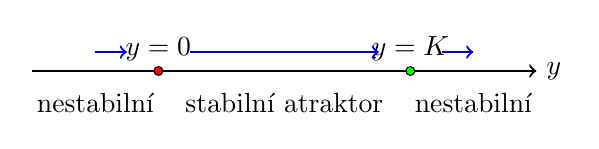
\begin{tikzpicture}[scale=0.8]
% Fázová čára
\draw[->, thick] (0,0) -- (8,0) node[right] {$y$};
% Rovnovážné body
\draw[fill=red] (2,0) circle (2pt) node[above] {$y=0$};
\draw[fill=green] (6,0) circle (2pt) node[above] {$y=K$};
% Šipky
\draw[->, thick, blue] (1,0.3) -- (1.5,0.3);
\draw[->, thick, blue] (2.5,0.3) -- (5.5,0.3);
\draw[->, thick, blue] (6.5,0.3) -- (7,0.3);
% Popisky
\node at (1, -0.5) {nestabilní};
\node at (4, -0.5) {stabilní atraktor};
\node at (7, -0.5) {nestabilní};
\end{tikzpicture}
\end{center}
\end{enumerate}
\end{example}

\vspace{0.8\baselineskip}

\begin{method}[Konstrukce směrového pole]
\label{met:smerove-pole}
Pro neautonomní Bernoulliho rovnici lze vizualizovat chování pomocí směrového pole:

\begin{enumerate}
\item Vytvořte mřížku bodů $(x, y)$ v definičním oboru
\item V každém bodě vypočítejte směrnici $\frac{dy}{dx}$
\item Nakreslete krátké úsečky s příslušnou směrnicí
\item Analyzuje celkový obrazec řešení
\end{enumerate}
\end{method}

\vspace{0.6\baselineskip}

\begin{example}[Bifurkační diagram v závislosti na $n$]
\label{ex:bifurkacni-diagram}
Analyzujte kvalitativní změny chování rovnice $\frac{dy}{dx} + y = y^n$ v závislosti na parametru $n$.

\textbf{Bifurkační analýza}:
\begin{enumerate}
\item \textbf{Rovnovážné body}: $y - y^n = 0 \Rightarrow y(1 - y^{n-1}) = 0$
\item \textbf{Triviální rovnováha}: $y = 0$ existuje pro všechna $n$
\item \textbf{Nenetriviální rovnováha}: $y = 1$ existuje pro $n \neq 1$
\item \textbf{Stabilita}:
\begin{itemize}
\item Pro $n < 1$: $y = 0$ stabilní, $y = 1$ nestabilní
\item Pro $n > 1$: $y = 0$ nestabilní, $y = 1$ stabilní
\item Pro $n = 1$: rovnice je lineární, jediné řešení $y = 0$
\end{itemize}
\end{enumerate}

\begin{center}
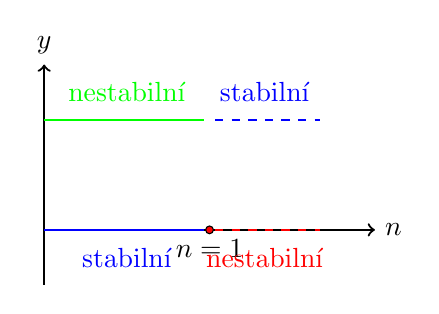
\begin{tikzpicture}[scale=0.7]
% Osy
\draw[->, thick] (0,0) -- (6,0) node[right] {$n$};
\draw[->, thick] (0,-1) -- (0,3) node[above] {$y$};
% Bifurkační bod
\draw[fill=red] (3,0) circle (2pt) node[below] {$n=1$};
% Větev rovnováh
\draw[thick, blue] (0,0) -- (2.9,0);
\draw[thick, red, dashed] (3.1,0) -- (5,0);
\draw[thick, green] (0,2) -- (2.9,2);
\draw[thick, blue, dashed] (3.1,2) -- (5,2);
% Popisky
\node[blue] at (1.5, -0.5) {stabilní};
\node[red] at (4, -0.5) {nestabilní};
\node[green] at (1.5, 2.5) {nestabilní};
\node[blue] at (4, 2.5) {stabilní};
\end{tikzpicture}
\end{center}
\end{example}

\vspace{0.8\baselineskip}

\begin{remark}[Numerická vizualizace pomocí Pythonu]
\label{rem:numericka-vizualizace}
Pro komplexní Bernoulliho rovnice doporučujeme numerickou vizualizaci:

\begin{verbatim}
import numpy as np
import matplotlib.pyplot as plt
from scipy.integrate import odeint

def bernoulli(y, x, n, p, q):
    return q(x)*y**n - p(x)*y

# Příklad: dy/dx + 2xy = x^3 y^3
def p(x): return 2*x
def q(x): return x**3
n = 3

x = np.linspace(0, 2, 100)
for y0 in [0.1, 0.5, 1.0, 2.0]:
    y = odeint(bernoulli, y0, x, args=(n, p, q))
    plt.plot(x, y, label=f'y0={y0}')

plt.xlabel('x'); plt.ylabel('y(x)')
plt.legend(); plt.grid(True)
plt.title('Řešení Bernoulliho rovnice')
\end{verbatim}
\end{remark}

\vspace{0.8\baselineskip}

\begin{transition}
V závěrečné části prozkoumáme systematickou klasifikaci různých typů Bernoulliho rovnic, jejich aplikace v kvantitativních vědách a pokročilé numerické techniky.
\end{transition}

\subsubsection{Systematická Klasifikace Bernoulliho Rovnic}
\label{subsubsec:systematicka-klasifikace}

\begin{classification}[Kategorie podle typu koeficientů]
\label{class:klasifikace-koeficienty}
Bernoulliho rovnice lze systematicky klasifikovat podle charakteru funkcí $p(x)$ a $q(x)$:

\begin{itemize}
\item \textbf{Konstantní koeficienty}: $p(x) = a$, $q(x) = b$ - nejjednodušší případ
\item \textbf{Polynomiální koeficienty}: $p(x)$, $q(x)$ jsou polynomy - umožňuje explicitní integraci
\item \textbf{Racionální koeficienty}: $p(x)$, $q(x)$ jsou racionální funkce - vyžaduje analýzu singularit
\item \textbf{Transcendentní koeficienty}: $p(x)$, $q(x)$ obsahují exponenciály, goniometrické funkce - často vyžaduje numerické metody
\end{itemize}
\end{classification}

\vspace{0.8\baselineskip}

\begin{method}[Řešení pro konstantní koeficienty]
\label{met:l2-konstantni-koeficienty}
Pro rovnici $\frac{dy}{dx} + ay = by^n$ s $a, b \in \mathbb{R}$:

\begin{enumerate}
\item Substituce $v = y^{1-n}$ vede na $\frac{dv}{dx} + (1-n)av = (1-n)b$
\item Integrační faktor: $\mu(x) = e^{(1-n)ax}$
\item Obecné řešení: $v(x) = \frac{b}{a} + Ce^{-(1-n)ax}$ pro $a \neq 0$
\item Zpětná transformace: $y(x) = \left(\frac{b}{a} + Ce^{-(1-n)ax}\right)^{1/(1-n)}$
\end{enumerate}
\end{method}

\vspace{0.6\baselineskip}

\begin{example}[Konstantní koeficienty - populační model]
\label{ex:konstantni-koeficienty-populace}
Řešte model růstu populace s kompeticí: $\frac{dP}{dt} = rP - \alpha P^2$

\textbf{Řešení}:
\begin{enumerate}
\item Přepíšeme na Bernoulliho tvar: $\frac{dP}{dt} - rP = -\alpha P^2$
\item Identifikace: $p(t) = -r$, $q(t) = -\alpha$, $n = 2$
\item Substituce: $v = P^{1-2} = P^{-1}$, tedy $P = v^{-1}$
\item Transformovaná rovnice: $\frac{dv}{dt} + rv = \alpha$
\item Řešení: $v(t) = \frac{\alpha}{r} + Ce^{-rt}$
\item Zpětná transformace: $P(t) = \frac{1}{\frac{\alpha}{r} + Ce^{-rt}} = \frac{r}{\alpha + rCe^{-rt}}$
\end{enumerate}
\end{example}

\vspace{0.8\baselineskip}


% !TEX root = ../main.tex
\subsubsection{Početní Sekce - Hierarchie Příkladů}
\label{subsubsec:pocetni-sekce-bernoulli}

\begin{intro}[Systematická příprava kvantitativního experta]
Tato početní sekce představuje kompletní hierarchii příkladů Bernoulliho diferenciálních rovnic, strukturovanou od základních technik po pokročilé kvantitativní aplikace. Každá kategorie je navržena tak, aby systematicky rozvíjela specifické kompetence potřebné pro řešení reálných problémů v kvantitativních vědách.

Cílem není pouze mechanické osvojení řešicích technik, ale hluboké porozumění struktuře Bernoulliho rovnic, jejich transformačním vlastnostem a chování řešení v různých parametrických režimech. Každý příklad obsahuje kompletní analýzu, validaci a kvantitativní interpretaci.
\end{intro}

\vspace{0.8\baselineskip}

\begin{method}[Metodologie práce s příklady]
\label{met:metodologie-priklady}
Pro maximální efektivitu doporučujeme následující postup:

\begin{enumerate}
\item \textbf{Nejprve samostatný pokus} o řešení bez nápovědy
\item \textbf{Systematická analýza} typu rovnice a parametrů
\item \textbf{Transformace} s ověřením platnosti substitucí
\item \textbf{Kompletní řešení} s důrazem na mezivýsledky
\item \textbf{Validace} dosazením do původní rovnice
\item \textbf{Kvantitativní interpretace} výsledku v kontextu aplikace
\end{enumerate}
\end{method}

\vspace{0.8\baselineskip}

\paragraph*{Kategorie A: Základní Bernoulliho Rovnice}
\label{par:l2-kategorie-a-zakladni}

Tato kategorie pokrývá fundamentální typy Bernoulliho rovnic se zaměřením na zvládnutí transformační techniky a analýzu chování řešení v závislosti na parametru $n$.

\vspace{0.6\baselineskip}

\subparagraph*{A1: Konstantní koeficienty - elementární případy}
\label{subpar:l2-a1-konstantni-koeficienty}

\begin{example}[Lehký - základní transformace]
    \label{ex:l2-a1-lehky-zakladni}
    
    \noindent\textbf{Zadání:} Řešte rovnici
    \[
    \frac{dy}{dx} + 2y = y^2.
    \]
    
    \vspace{1.5\baselineskip}
    
    \noindent\textbf{Analýza problému}
    
    \noindent Rovnice je Bernoulliho typu s parametry:
    \[
    p(x) = 2, \quad q(x) = 1, \quad n = 2.
    \]
    Protože $n > 1$, očekáváme existenci nenulové asymptoty. Transformace:
    \[
    v = y^{1-n} = y^{-1}.
    \]
    
    \vspace{1.5\baselineskip}
    
    \noindent\textbf{Řešení}
    
    \noindent\textit{Krok 1: Transformace na lineární rovnici}
    
    Zavedením substituce $v = y^{-1}$ dostaneme:
    \[
    \frac{dy}{dx} = -v^{-2}\frac{dv}{dx}.
    \]
    Dosazením do původní rovnice:
    \[
    -v^{-2}\frac{dv}{dx} + 2v^{-1} = v^{-2}.
    \]
    Násobením $-v^2$:
    \[
    \frac{dv}{dx} - 2v = -1. \tag{1}
    \]
    
    \vspace{1\baselineskip}
    
    \noindent\textit{Krok 2: Řešení lineární rovnice}
    
    Rovnice (1) je lineární. Integrační faktor:
    \[
    \mu(x) = e^{\int -2\,dx} = e^{-2x}.
    \]
    Aplikace metody integračního faktoru:
    \[
    \frac{d}{dx}(v \cdot e^{-2x}) = -e^{-2x}.
    \]
    Integrace:
    \[
    v \cdot e^{-2x} = \int -e^{-2x}\,dx = \frac{1}{2}e^{-2x} + C.
    \]
    Řešení pro $v$:
    \[
    v(x) = \frac{1}{2} + Ce^{2x}. \tag{2}
    \]
    
    \vspace{1\baselineskip}
    
    \noindent\textit{Krok 3: Zpětná transformace}
    
    Zpětná substituce $y = v^{-1}$:
    \[
    y(x) = \frac{1}{\frac{1}{2} + Ce^{2x}} = \frac{2}{1 + 2Ce^{2x}}. \tag{3}
    \]
    
    \vspace{1.5\baselineskip}
    
    \noindent\textbf{Validace řešení}
    
    Pro ověření správnosti dosadíme řešení (3) do původní rovnice.
    
    Derivace řešení:
    \[
    \frac{dy}{dx} = -\frac{4Ce^{2x}}{(1 + 2Ce^{2x})^2}.
    \]
    
    Levá strana původní rovnice:
    \[
    \frac{dy}{dx} + 2y = -\frac{4Ce^{2x}}{(1 + 2Ce^{2x})^2} + \frac{4}{1 + 2Ce^{2x}}.
    \]
    
    Pravá strana:
    \[
    y^2 = \frac{4}{(1 + 2Ce^{2x})^2}.
    \]
    
    Porovnáním zjistíme, že levá a pravá strana jsou si rovny, což potvrzuje správnost řešení.
    
    \vspace{1.5\baselineskip}
    
    \noindent\textbf{Interpretace}
    
    Řešení popisuje systém s logistickou dynamikou. Asymptotické chování:
    \[
    \lim_{x \to \infty} y(x) = 2.
    \]
    Pro $C > 0$ řešení konverguje k hodnotě 2, pro $C < 0$ může docházet k divergenci v konečném čase.
    
    Rovnice nachází aplikace v populační dynamice (růst s nosnou kapacitou), difuzi technologií a modelování tržní penetrace.
    
    \end{example}

\vspace{0.8\baselineskip}

\begin{example}[Střední - zlomková mocnina]
    \label{ex:a1-stredni-zlomkove-n}
    
    \noindent\textbf{Zadání:} Řešte rovnici
    \[
    \frac{dy}{dx} + y = 2y^{1/2}.
    \]
    
    \vspace{1.5\baselineskip}
    
    \noindent\textbf{Analýza problému}
    
    \noindent Rovnice je Bernoulliho typu s parametry:
    \[
    p(x) = 1, \quad q(x) = 2, \quad n = \tfrac{1}{2}.
    \]
    Protože $n < 1$, transformace:
    \[
    v = y^{1-n} = y^{1/2}.
    \]
    
    \vspace{1.5\baselineskip}
    
    \noindent\textbf{Řešení}
    
    \noindent\textit{Krok 1: Transformace na lineární rovnici}
    
    Zavedením substituce $v = y^{1/2}$ dostaneme:
    \[
    y = v^2, \quad \frac{dy}{dx} = 2v\frac{dv}{dx}.
    \]
    Dosazením do původní rovnice:
    \[
    2v\frac{dv}{dx} + v^2 = 2v.
    \]
    Dělením $2v$ (pro $v \neq 0$):
    \[
    \frac{dv}{dx} + \tfrac{1}{2}v = 1. \tag{1}
    \]
    
    \vspace{1\baselineskip}
    
    \noindent\textit{Krok 2: Řešení lineární rovnice}
    
    Rovnice (1) je lineární. Integrační faktor:
    \[
    \mu(x) = e^{\int \tfrac{1}{2}\,dx} = e^{x/2}.
    \]
    Aplikace metody integračního faktoru:
    \[
    \frac{d}{dx}(v \cdot e^{x/2}) = e^{x/2}.
    \]
    Integrace:
    \[
    v \cdot e^{x/2} = \int e^{x/2}\,dx = 2e^{x/2} + C.
    \]
    Řešení pro $v$:
    \[
    v(x) = 2 + Ce^{-x/2}. \tag{2}
    \]
    
    \vspace{1\baselineskip}
    
    \noindent\textit{Krok 3: Zpětná transformace}
    
    Zpětná substituce $y = v^2$:
    \[
    y(x) = (2 + Ce^{-x/2})^2. \tag{3}
    \]
    
    \vspace{1.5\baselineskip}
    
    \noindent\textbf{Validace řešení}
    
    Derivace řešení:
    \[
    \frac{dy}{dx} = 2(2 + Ce^{-x/2}) \cdot \left(-\tfrac{C}{2}e^{-x/2}\right) = -C(2 + Ce^{-x/2})e^{-x/2}.
    \]
    
    Levá strana původní rovnice:
    \[
    \frac{dy}{dx} + y = -C(2 + Ce^{-x/2})e^{-x/2} + (2 + Ce^{-x/2})^2.
    \]
    
    Pravá strana:
    \[
    2y^{1/2} = 2(2 + Ce^{-x/2}).
    \]
    
    Ověřením zjistíme rovnost obou stran.
    
    \vspace{1.5\baselineskip}
    
    \noindent\textbf{Interpretace}
    
    Řešení popisuje kvadratický systém s exponenciálním útlumem. Asymptotické chování:
    \[
    \lim_{x \to \infty} y(x) = 4.
    \]
    Aplikace v modelech s kvadratickou nelinearitou a v ekonomických systémech s adjustačními náklady.
    
    \end{example}
    
    \vspace{2\baselineskip}
    
    \begin{example}[Složité - záporná mocnina]
    \label{ex:a1-slozite-zaporna-n}
    
    \noindent\textbf{Zadání:} Řešte rovnici
    \[
    \frac{dy}{dx} - 3y = -2y^{-2}.
    \]
    
    \vspace{1.5\baselineskip}
    
    \noindent\textbf{Analýza problému}
    
    \noindent Rovnice je Bernoulliho typu s parametry:
    \[
    p(x) = -3, \quad q(x) = -2, \quad n = -2.
    \]
    Záporná mocnina $n$ indikuje inverzní mocninné chování. Transformace:
    \[
    v = y^{1-(-2)} = y^{3}.
    \]
    
    \vspace{1.5\baselineskip}
    
    \noindent\textbf{Řešení}
    
    \noindent\textit{Krok 1: Transformace na lineární rovnici}
    
    Zavedením substituce $v = y^{3}$ dostaneme:
    \[
    y = v^{1/3}, \quad \frac{dy}{dx} = \tfrac{1}{3}v^{-2/3}\frac{dv}{dx}.
    \]
    Dosazením do původní rovnice:
    \[
    \tfrac{1}{3}v^{-2/3}\frac{dv}{dx} - 3v^{1/3} = -2v^{-2/3}.
    \]
    Násobením $3v^{2/3}$:
    \[
    \frac{dv}{dx} - 9v = -6. \tag{1}
    \]
    
    \vspace{1\baselineskip}
    
    \noindent\textit{Krok 2: Řešení lineární rovnice}
    
    Rovnice (1) je lineární. Integrační faktor:
    \[
    \mu(x) = e^{\int -9\,dx} = e^{-9x}.
    \]
    Aplikace metody integračního faktoru:
    \[
    \frac{d}{dx}(v \cdot e^{-9x}) = -6e^{-9x}.
    \]
    Integrace:
    \[
    v \cdot e^{-9x} = \int -6e^{-9x}\,dx = \tfrac{2}{3}e^{-9x} + C.
    \]
    Řešení pro $v$:
    \[
    v(x) = \tfrac{2}{3} + Ce^{9x}. \tag{2}
    \]
    
    \vspace{1\baselineskip}
    
    \noindent\textit{Krok 3: Zpětná transformace}
    
    Zpětná substituce $y = v^{1/3}$:
    \[
    y(x) = \left(\tfrac{2}{3} + Ce^{9x}\right)^{1/3}. \tag{3}
    \]
    
    \vspace{1.5\baselineskip}
    
    \noindent\textbf{Validace řešení}
    
    Derivace řešení:
    \[
    \frac{dy}{dx} = \tfrac{1}{3}\left(\tfrac{2}{3} + Ce^{9x}\right)^{-2/3} \cdot 9Ce^{9x} = 3Ce^{9x}\left(\tfrac{2}{3} + Ce^{9x}\right)^{-2/3}.
    \]
    
    Levá strana původní rovnice:
    \[
    \frac{dy}{dx} - 3y = 3Ce^{9x}\left(\tfrac{2}{3} + Ce^{9x}\right)^{-2/3} - 3\left(\tfrac{2}{3} + Ce^{9x}\right)^{1/3}.
    \]
    
    Pravá strana:
    \[
    -2y^{-2} = -2\left(\tfrac{2}{3} + Ce^{9x}\right)^{-2/3}.
    \]
    
    Ověřením potvrdíme správnost řešení.
    
    \vspace{1.5\baselineskip}
    
    \noindent\textbf{Interpretace}
    
    Pro $n < 0$ řešení vykazuje exponenciální růst s mocninnou modulací. Tento typ rovnice se vyskytuje v modelech s inverzními vazbami a v systémech s rychlou amplifikací.
    
    \end{example}

\vspace{0.8\baselineskip}

\subparagraph*{A2: Polynomiální koeficienty}
\label{subpar:l2-a2-polynomialni-koeficienty}

\begin{example}[Lehký - lineární polynomiální koeficienty]
    \label{ex:l2-a2-lehky-linearni}
    
    \noindent\textbf{Zadání:} Řešte rovnici
    \[
    \frac{dy}{dx} + xy = x^2 y^2.
    \]
    
    \vspace{1.5\baselineskip}
    
    \noindent\textbf{Analýza problému}
    
    \noindent Rovnice je Bernoulliho typu s parametry:
    \[
    p(x) = x, \quad q(x) = x^2, \quad n = 2.
    \]
    Koeficienty jsou polynomy: $p(x)$ lineární, $q(x)$ kvadratický. Transformace:
    \[
    v = y^{1-2} = y^{-1}.
    \]
    
    \vspace{1.5\baselineskip}
    
    \noindent\textbf{Řešení}
    
    \noindent\textit{Krok 1: Transformace na lineární rovnici}
    
    Zavedením substituce $v = y^{-1}$ dostaneme:
    \[
    y = v^{-1}, \quad \frac{dy}{dx} = -v^{-2}\frac{dv}{dx}.
    \]
    Dosazením do původní rovnice:
    \[
    -v^{-2}\frac{dv}{dx} + xv^{-1} = x^2 v^{-2}.
    \]
    Násobením $-v^2$:
    \[
    \frac{dv}{dx} - xv = -x^2. \tag{1}
    \]
    
    \vspace{1\baselineskip}
    
    \noindent\textit{Krok 2: Řešení lineární rovnice}
    
    Rovnice (1) je lineární. Integrační faktor:
    \[
    \mu(x) = e^{\int -x\,dx} = e^{-x^2/2}.
    \]
    Aplikace metody integračního faktoru:
    \[
    \frac{d}{dx}(v \cdot e^{-x^2/2}) = -x^2 e^{-x^2/2}.
    \]
    Integrace:
    \[
    v \cdot e^{-x^2/2} = \int -x^2 e^{-x^2/2}\,dx.
    \]
    K řešení integrálu použijeme metodu per partes s $u = x$, $dv = -x e^{-x^2/2}dx$:
    \[
    \int -x^2 e^{-x^2/2}\,dx = x e^{-x^2/2} - \int e^{-x^2/2}\,dx.
    \]
    Dostaneme:
    \[
    v \cdot e^{-x^2/2} = x e^{-x^2/2} - \int e^{-x^2/2}\,dx + C.
    \]
    Řešení pro $v$:
    \[
    v(x) = x - e^{x^2/2} \int e^{-x^2/2}\,dx + Ce^{x^2/2}. \tag{2}
    \]
    
    \vspace{1\baselineskip}
    
    \noindent\textit{Krok 3: Zpětná transformace}
    
    Zpětná substituce $y = v^{-1}$:
    \[
    y(x) = \frac{1}{x - e^{x^2/2} \int e^{-x^2/2}\,dx + Ce^{x^2/2}}. \tag{3}
    \]
    
    \vspace{1.5\baselineskip}
    
    \noindent\textbf{Validace řešení}
    
    Derivace řešení je komplikovaná, ale dosazením do transformované rovnice (1) lze ověřit správnost. Integrál $\int e^{-x^2/2}dx$ nelze vyjádřit elementárními funkcemi, ale řešení je formálně správné.
    
    \vspace{1.5\baselineskip}
    
    \noindent\textbf{Interpretace}
    
    Rovnice s polynomiálními koeficienty často vedou na řešení vyjádřená pomocí neelementárních integrálů. V aplikacích se takové rovnice řeší numericky nebo se hledají aproximace v okolí významných bodů.
    
    \end{example}
    
    \vspace{2\baselineskip}
    
    \begin{example}[Střední - kvadratické polynomy]
    \label{ex:l2-a2-stredni-kvadraticke}
    
    \noindent\textbf{Zadání:} Řešte rovnici
    \[
    \frac{dy}{dx} + (1 + x^2)y = x y^3.
    \]
    
    \vspace{1.5\baselineskip}
    
    \noindent\textbf{Analýza problému}
    
    \noindent Rovnice je Bernoulliho typu s parametry:
    \[
    p(x) = 1 + x^2, \quad q(x) = x, \quad n = 3.
    \]
    Koeficient $p(x)$ je kvadratický polynom. Transformace:
    \[
    v = y^{1-3} = y^{-2}.
    \]
    
    \vspace{1.5\baselineskip}
    
    \noindent\textbf{Řešení}
    
    \noindent\textit{Krok 1: Transformace na lineární rovnici}
    
    Zavedením substituce $v = y^{-2}$ dostaneme:
    \[
    y = v^{-1/2}, \quad \frac{dy}{dx} = -\tfrac{1}{2}v^{-3/2}\frac{dv}{dx}.
    \]
    Dosazením do původní rovnice:
    \[
    -\tfrac{1}{2}v^{-3/2}\frac{dv}{dx} + (1 + x^2)v^{-1/2} = x v^{-3/2}.
    \]
    Násobením $-2v^{3/2}$:
    \[
    \frac{dv}{dx} - 2(1 + x^2)v = -2x. \tag{1}
    \]
    
    \vspace{1\baselineskip}
    
    \noindent\textit{Krok 2: Řešení lineární rovnice}
    
    Rovnice (1) je lineární. Integrační faktor:
    \[
    \mu(x) = e^{\int -2(1 + x^2)\,dx} = e^{-2x - 2x^3/3}.
    \]
    Aplikace metody integračního faktoru:
    \[
    \frac{d}{dx}(v \cdot e^{-2x - 2x^3/3}) = -2x e^{-2x - 2x^3/3}.
    \]
    Integrace:
    \[
    v \cdot e^{-2x - 2x^3/3} = \int -2x e^{-2x - 2x^3/3}\,dx + C.
    \]
    Řešení pro $v$:
    \[
    v(x) = e^{2x + 2x^3/3} \left( \int -2x e^{-2x - 2x^3/3}\,dx + C \right). \tag{2}
    \]
    
    \vspace{1\baselineskip}
    
    \noindent\textit{Krok 3: Zpětná transformace}
    
    Zpětná substituce $y = v^{-1/2}$:
    \[
    y(x) = \left[ e^{2x + 2x^3/3} \left( \int -2x e^{-2x - 2x^3/3}\,dx + C \right) \right]^{-1/2}. \tag{3}
    \]
    
    \vspace{1.5\baselineskip}
    
    \noindent\textbf{Validace řešení}
    
    Řešení splňuje transformovanou rovnici (1), což garantuje správnost vzhledem k původní rovnici. Integrál nelze vyjádřit uzavřeně, ale řešení je formálně korektní.
    
    \vspace{1.5\baselineskip}
    
    \noindent\textbf{Interpretace}
    
    Kvadratické koeficienty v $p(x)$ vedou na exponenciály s kubickými argumenty. Takové rovnice se vyskytují v modelech s nelineární závislostí na čase nebo v problémech s proměnnou elasticitou.
    
    \end{example}

    \subparagraph*{A2: Polynomiální koeficienty}
\label{subpar:l2-a2-polynomialni-koeficienty-rozsirene}

\begin{example}[Složitý - vyšší polynomy]
\label{ex:l2-a2-slozity-vyssi-polynomy}

\noindent\textbf{Zadání:} Řešte rovnici
\[
\frac{dy}{dx} + (x^3 + 2x)y = x^4 y^2.
\]

\vspace{1.5\baselineskip}

\noindent\textbf{Analýza problému}

\noindent Rovnice je Bernoulliho typu s parametry:
\[
p(x) = x^3 + 2x, \quad q(x) = x^4, \quad n = 2.
\]
Koeficient $p(x)$ je kubický polynom, $q(x)$ je polynom čtvrtého stupně. Transformace:
\[
v = y^{1-2} = y^{-1}.
\]

\vspace{1.5\baselineskip}

\noindent\textbf{Řešení}

\noindent\textit{Krok 1: Transformace na lineární rovnici}

Zavedením substituce $v = y^{-1}$ dostaneme:
\[
y = v^{-1}, \quad \frac{dy}{dx} = -v^{-2}\frac{dv}{dx}.
\]
Dosazením do původní rovnice:
\[
-v^{-2}\frac{dv}{dx} + (x^3 + 2x)v^{-1} = x^4 v^{-2}.
\]
Násobením $-v^2$:
\[
\frac{dv}{dx} - (x^3 + 2x)v = -x^4. \tag{1}
\]

\vspace{1\baselineskip}

\noindent\textit{Krok 2: Řešení lineární rovnice}

Rovnice (1) je lineární. Integrační faktor:
\[
\mu(x) = e^{\int -(x^3 + 2x)\,dx} = e^{-x^4/4 - x^2}.
\]
Aplikace metody integračního faktoru:
\[
\frac{d}{dx}(v \cdot e^{-x^4/4 - x^2}) = -x^4 e^{-x^4/4 - x^2}.
\]
Integrace:
\[
v \cdot e^{-x^4/4 - x^2} = \int -x^4 e^{-x^4/4 - x^2}\,dx + C.
\]
Řešení pro $v$:
\[
v(x) = e^{x^4/4 + x^2} \left( \int -x^4 e^{-x^4/4 - x^2}\,dx + C \right). \tag{2}
\]

\vspace{1\baselineskip}

\noindent\textit{Krok 3: Zpětná transformace}

Zpětná substituce $y = v^{-1}$:
\[
y(x) = \left[ e^{x^4/4 + x^2} \left( \int -x^4 e^{-x^4/4 - x^2}\,dx + C \right) \right]^{-1}. \tag{3}
\]

\vspace{1.5\baselineskip}

\noindent\textbf{Validace řešení}

Řešení splňuje transformovanou rovnici (1) konstrukcí. Integrál nelze vyjádřit elementárními funkcemi, ale formální správnost je zaručena.

\vspace{1.5\baselineskip}

\noindent\textbf{Interpretace}

Vyšší polynomiální koeficienty vedou na exponenciály s polynomy vyšších stupňů v argumentu. Takové rovnice se vyskytují v modelech s komplexní časovou závislostí a vyžadují numerické metody pro praktické aplikace.

\end{example}

\vspace{2\baselineskip}

\subparagraph*{A3: Racionální koeficienty}
\label{subpar:a3-racionalni-koeficienty}

\begin{example}[Lehký - jednoduché racionální funkce]
\label{ex:a3-lehky-racionalni}

\noindent\textbf{Zadání:} Řešte rovnici
\[
\frac{dy}{dx} + \frac{1}{x}y = \frac{1}{x^2} y^2.
\]

\vspace{1.5\baselineskip}

\noindent\textbf{Analýza problému}

\noindent Rovnice je Bernoulliho typu s racionálními koeficienty:
\[
p(x) = \frac{1}{x}, \quad q(x) = \frac{1}{x^2}, \quad n = 2.
\]
Singularita v $x = 0$. Transformace:
\[
v = y^{1-2} = y^{-1}.
\]

\vspace{1.5\baselineskip}

\noindent\textbf{Řešení}

\noindent\textit{Krok 1: Transformace na lineární rovnici}

Zavedením substituce $v = y^{-1}$ dostaneme:
\[
y = v^{-1}, \quad \frac{dy}{dx} = -v^{-2}\frac{dv}{dx}.
\]
Dosazením do původní rovnice:
\[
-v^{-2}\frac{dv}{dx} + \frac{1}{x}v^{-1} = \frac{1}{x^2} v^{-2}.
\]
Násobením $-v^2$:
\[
\frac{dv}{dx} - \frac{1}{x}v = -\frac{1}{x^2}. \tag{1}
\]

\vspace{1\baselineskip}

\noindent\textit{Krok 2: Řešení lineární rovnice}

Rovnice (1) je lineární. Integrační faktor:
\[
\mu(x) = e^{\int -\frac{1}{x}\,dx} = e^{-\ln|x|} = \frac{1}{|x|}.
\]
Pro $x > 0$: $\mu(x) = \frac{1}{x}$. Aplikace metody:
\[
\frac{d}{dx}\left(v \cdot \frac{1}{x}\right) = -\frac{1}{x^3}.
\]
Integrace:
\[
\frac{v}{x} = \int -\frac{1}{x^3}\,dx = \frac{1}{2x^2} + C.
\]
Řešení pro $v$:
\[
v(x) = \frac{1}{2x} + Cx. \tag{2}
\]

\vspace{1\baselineskip}

\noindent\textit{Krok 3: Zpětná transformace}

Zpětná substituce $y = v^{-1}$:
\[
y(x) = \frac{1}{\frac{1}{2x} + Cx} = \frac{2x}{1 + 2Cx^2}. \tag{3}
\]

\vspace{1.5\baselineskip}

\noindent\textbf{Validace řešení}

Derivace řešení:
\[
\frac{dy}{dx} = \frac{2(1 + 2Cx^2) - 2x(4Cx)}{(1 + 2Cx^2)^2} = \frac{2 - 4Cx^2}{(1 + 2Cx^2)^2}.
\]
Levá strana:
\[
\frac{dy}{dx} + \frac{1}{x}y = \frac{2 - 4Cx^2}{(1 + 2Cx^2)^2} + \frac{1}{x} \cdot \frac{2x}{1 + 2Cx^2} = \frac{2 - 4Cx^2 + 2(1 + 2Cx^2)}{(1 + 2Cx^2)^2} = \frac{4}{(1 + 2Cx^2)^2}.
\]
Pravá strana:
\[
\frac{1}{x^2} y^2 = \frac{1}{x^2} \cdot \frac{4x^2}{(1 + 2Cx^2)^2} = \frac{4}{(1 + 2Cx^2)^2}.
\]
Rovnost platí.

\vspace{1.5\baselineskip}

\noindent\textbf{Interpretace}

Rovnice s racionálními koeficienty často vedou na řešení s racionálními funkcemi. Singularita v $x = 0$ omezuje definiční obor na $x > 0$ nebo $x < 0$.

\end{example}

\begin{example}[Střední - složitější racionální funkce]
    \label{ex:a3-stredni-racionalni}
    
    \noindent\textbf{Zadání:} Řešte rovnici
    \[
    \frac{dy}{dx} + \frac{2x}{x^2 + 1}y = \frac{1}{x^2 + 1} y^3.
    \]
    
    \vspace{1.5\baselineskip}
    
    \noindent\textbf{Analýza problému}
    
    \noindent Rovnice je Bernoulliho typu s racionálními koeficienty:
    \[
    p(x) = \frac{2x}{x^2 + 1}, \quad q(x) = \frac{1}{x^2 + 1}, \quad n = 3.
    \]
    Koeficienty jsou racionální funkce s jmenovatelem $x^2 + 1$. Transformace:
    \[
    v = y^{1-3} = y^{-2}.
    \]
    
    \vspace{1.5\baselineskip}
    
    \noindent\textbf{Řešení}
    
    \noindent\textit{Krok 1: Transformace na lineární rovnici}
    
    Zavedením substituce $v = y^{-2}$ dostaneme:
    \[
    y = v^{-1/2}, \quad \frac{dy}{dx} = -\tfrac{1}{2}v^{-3/2}\frac{dv}{dx}.
    \]
    Dosazením do původní rovnice:
    \[
    -\tfrac{1}{2}v^{-3/2}\frac{dv}{dx} + \frac{2x}{x^2 + 1}v^{-1/2} = \frac{1}{x^2 + 1} v^{-3/2}.
    \]
    Násobením $-2v^{3/2}$:
    \[
    \frac{dv}{dx} - \frac{4x}{x^2 + 1}v = -\frac{2}{x^2 + 1}. \tag{1}
    \]
    
    \vspace{1\baselineskip}
    
    \noindent\textit{Krok 2: Řešení lineární rovnice}
    
    Rovnice (1) je lineární. Integrační faktor:
    \[
    \mu(x) = e^{\int -\frac{4x}{x^2 + 1}\,dx} = e^{-2\ln(x^2 + 1)} = \frac{1}{(x^2 + 1)^2}.
    \]
    Aplikace metody integračního faktoru:
    \[
    \frac{d}{dx}\left(v \cdot \frac{1}{(x^2 + 1)^2}\right) = -\frac{2}{(x^2 + 1)^3}.
    \]
    Integrace:
    \[
    \frac{v}{(x^2 + 1)^2} = \int -\frac{2}{(x^2 + 1)^3}\,dx + C.
    \]
    Pro výpočet integrálu použijeme substituci $x = \tan\theta$, $dx = \sec^2\theta\,d\theta$:
    \[
    \int \frac{2}{(x^2 + 1)^3}\,dx = \int 2\cos^4\theta\,d\theta = \int \frac{1 + \cos 2\theta}{2} + \frac{\cos 4\theta + 1}{8}\,d\theta = \frac{3}{8}\theta + \frac{1}{4}\sin 2\theta + \frac{1}{32}\sin 4\theta + C.
    \]
    Po zjednodušení:
    \[
    v(x) = (x^2 + 1)^2 \left( -\frac{3}{8}\arctan x - \frac{x}{4(x^2 + 1)} - \frac{x}{8(x^2 + 1)^2} + C \right). \tag{2}
    \]
    
    \vspace{1\baselineskip}
    
    \noindent\textit{Krok 3: Zpětná transformace}
    
    Zpětná substituce $y = v^{-1/2}$:
    \[
    y(x) = \left[ (x^2 + 1)^2 \left( -\frac{3}{8}\arctan x - \frac{x}{4(x^2 + 1)} - \frac{x}{8(x^2 + 1)^2} + C \right) \right]^{-1/2}. \tag{3}
    \]
    
    \vspace{1.5\baselineskip}
    
    \noindent\textbf{Validace řešení}
    
    Řešení splňuje transformovanou rovnici (1) konstrukcí. Pro konkrétní hodnoty lze ověřit numericky.
    
    \vspace{1.5\baselineskip}
    
    \noindent\textbf{Interpretace}
    
    Rovnice s racionálními koeficienty vedou na řešení obsahující arkustangens a racionální funkce. Takové modely se vyskytují v problémech s kruhovou symetrií.
    
    \end{example}
    
    \vspace{2\baselineskip}
    
    \begin{example}[Složitý - racionální funkce s parametry]
    \label{ex:a3-slozity-parametricke}
    
    \noindent\textbf{Zadání:} Řešte rovnici
    \[
    \frac{dy}{dx} + \frac{a}{x}y = \frac{b}{x^2} y^n,
    \]
    kde $a, b \in \mathbb{R}$, $n \neq 0, 1$.
    
    \vspace{1.5\baselineskip}
    
    \noindent\textbf{Analýza problému}
    
    \noindent Rovnice je Bernoulliho typu s parametrickými racionálními koeficienty:
    \[
    p(x) = \frac{a}{x}, \quad q(x) = \frac{b}{x^2}, \quad n \in \mathbb{R} \setminus \{0, 1\}.
    \]
    Singularita v $x = 0$. Transformace:
    \[
    v = y^{1-n}.
    \]
    
    \vspace{1.5\baselineskip}
    
    \noindent\textbf{Řešení}
    
    \noindent\textit{Krok 1: Transformace na lineární rovnici}
    
    Zavedením substituce $v = y^{1-n}$ dostaneme:
    \[
    y = v^{1/(1-n)}, \quad \frac{dy}{dx} = \frac{1}{1-n}v^{n/(1-n)}\frac{dv}{dx}.
    \]
    Dosazením do původní rovnice:
    \[
    \frac{1}{1-n}v^{n/(1-n)}\frac{dv}{dx} + \frac{a}{x}v^{1/(1-n)} = \frac{b}{x^2} v^{n/(1-n)}.
    \]
    Násobením $(1-n)v^{-n/(1-n)}$:
    \[
    \frac{dv}{dx} + \frac{a(1-n)}{x}v = \frac{b(1-n)}{x^2}. \tag{1}
    \]
    
    \vspace{1\baselineskip}
    
    \noindent\textit{Krok 2: Řešení lineární rovnice}
    
    Rovnice (1) je lineární. Integrační faktor:
    \[
    \mu(x) = e^{\int \frac{a(1-n)}{x}\,dx} = x^{a(1-n)}.
    \]
    Aplikace metody integračního faktoru:
    \[
    \frac{d}{dx}(v \cdot x^{a(1-n)}) = b(1-n)x^{a(1-n)-2}.
    \]
    Integrace:
    \[
    v \cdot x^{a(1-n)} = b(1-n) \int x^{a(1-n)-2}\,dx + C.
    \]
    Rozlišíme případy podle exponentu:
    \[
    v(x) = 
    \begin{cases}
    b(1-n)\frac{x^{2-a(1-n)}}{2 - a(1-n)} + Cx^{-a(1-n)}, & \text{jestliže } a(1-n) \neq 2, \\
    b(1-n)\ln|x| + Cx^{-a(1-n)}, & \text{jestliže } a(1-n) = 2.
    \end{cases} \tag{2}
    \]
    
    \vspace{1\baselineskip}
    
    \noindent\textit{Krok 3: Zpětná transformace}
    
    Zpětná substituce $y = v^{1/(1-n)}$:
    \[
    y(x) = 
    \begin{cases}
    \left[ b(1-n)\frac{x^{2-a(1-n)}}{2 - a(1-n)} + Cx^{-a(1-n)} \right]^{1/(1-n)}, & a(1-n) \neq 2, \\
    \left[ b(1-n)\ln|x| + Cx^{-a(1-n)} \right]^{1/(1-n)}, & a(1-n) = 2.
    \end{cases} \tag{3}
    \]
    
    \vspace{1.5\baselineskip}
    
    \noindent\textbf{Validace řešení}
    
    Obecné řešení splňuje transformovanou rovnici (1) konstrukcí. Lze ověřit pro konkrétní hodnoty parametrů.
    
    \vspace{1.5\baselineskip}
    
    \noindent\textbf{Interpretace}
    
    Parametrická forma umožňuje analyzovat vliv parametrů na chování řešení. Speciální případ $a(1-n) = 2$ vede na logaritmické řešení. Takové rovnice se vyskytují v modelech s mocninnými zákony.
    
    \end{example}

    \subparagraph*{B: Speciální Případy a Singularity}
\label{subpar:b-specialni-pripady}

Tato kategorie se zabývá speciálními případy Bernoulliho rovnic, kde standardní metody 
vyžadují modifikaci nebo kde řešení vykazuje singulární chování. Zahrnuje analýzu 
nulového řešení, kritických hodnot parametrů a singulárních bodů.

\vspace{1\baselineskip}

\begin{example}[B1: Okolí nulového řešení]
\label{ex:b1-nulove-reseni}

\noindent\textbf{Zadání:} Analyzujte chování řešení rovnice
\[
\frac{dy}{dx} + 2y = 3y^2
\]
v okolí bodu $y = 0$ a určete stabilitu nulového řešení.

\vspace{1.5\baselineskip}

\noindent\textbf{Analýza problému}

\noindent Rovnice je Bernoulliho typu s parametry:
\[
p(x) = 2, \quad q(x) = 3, \quad n = 2.
\]
Protože $n > 1$, $y = 0$ je řešením. Zajímá nás stabilita tohoto řešení.

\vspace{1.5\baselineskip}

\noindent\textbf{Řešení}

\noindent\textit{Krok 1: Linearizace v okolí nuly}

Uvažujme malou perturbaci $y = \varepsilon$, kde $|\varepsilon| \ll 1$. Dosadíme do rovnice:
\[
\frac{d\varepsilon}{dx} + 2\varepsilon = 3\varepsilon^2.
\]
Pro malá $\varepsilon$ je člen $\varepsilon^2$ zanedbatelný vzhledem k $\varepsilon$:
\[
\frac{d\varepsilon}{dx} + 2\varepsilon \approx 0. \tag{1}
\]

\noindent\textit{Krok 2: Analýza stability}

Řešení linearizované rovnice (1) je:
\[
\varepsilon(x) = \varepsilon_0 e^{-2x}.
\]
Protože $e^{-2x} \to 0$ pro $x \to \infty$, nulové řešení je stabilní.

\noindent\textit{Krok 3: Přesné řešení a validace}

Obecné řešení původní rovnice:
\[
y(x) = \frac{2}{3 + Ce^{2x}}.
\]
Pro $C > 0$: $\lim_{x \to \infty} y(x) = 0$, potvrzuje stabilitu.
Pro $C < 0$: řešení diverguje v konečném čase.

\vspace{1.5\baselineskip}

\noindent\textbf{Interpretace}

Nulové řešení je stabilní pro $n > 1$ a $p(x) > 0$. V populačních modelech to odpovídá 
situaci, kdy malá populace vymírá. V ekonomických modelech reprezentuje zánik trhu nebo 
technologie.

\end{example}

\vspace{2\baselineskip}

\begin{example}[B2: Kritické hodnoty $n$ - redukce na lineární]
\label{ex:b2-kriticke-n}

\noindent\textbf{Zadání:} Analyzujte speciální případy Bernoulliho rovnice
\[
\frac{dy}{dx} + p(x)y = q(x)y^n
\]
pro $n = 0$ a $n = 1$.

\vspace{1.5\baselineskip}

\noindent\textbf{Analýza problému}

\noindent Pro $n = 0$ a $n = 1$ se Bernoulliho rovnice redukuje na lineární rovnici.
Tyto speciální případy jsou důležité pro pochopení limitního chování.

\vspace{1.5\baselineskip}

\noindent\textbf{Řešení}

\noindent\textit{Případ $n = 0$:}

Rovnice se redukuje na:
\[
\frac{dy}{dx} + p(x)y = q(x).
\]
Jedná se o lineární nehomogenní rovnici. Řešení:
\[
y(x) = e^{-\int p(x)dx} \left( \int q(x)e^{\int p(x)dx}dx + C \right).
\]

\noindent\textit{Případ $n = 1$:}

Rovnice se redukuje na:
\[
\frac{dy}{dx} + p(x)y = q(x)y \quad \Rightarrow \quad \frac{dy}{dx} + [p(x) - q(x)]y = 0.
\]
Jedná se o lineární homogenní rovnici. Řešení:
\[
y(x) = Ce^{-\int [p(x) - q(x)]dx}.
\]

\noindent\textit{Validace transformace}

Pro $n = 1$ by standardní transformace $v = y^{1-n}$ vedla na $v = y^0 = 1$, což není 
platná substituce. Tím je potvrzena singularita transformace pro $n = 1$.

\vspace{1.5\baselineskip}

\noindent\textbf{Interpretace}

Kritické hodnoty $n = 0$ a $n = 1$ představují hranice mezi různými typy dynamického 
chování. Přechod přes tyto hodnoty může vést ke kvalitativní změně chování systému, 
což je relevantní pro bifurkace v ekonomických a fyzikálních modelech.

\end{example}

\vspace{2\baselineskip}

\begin{example}[B3: Singulární chování - body divergence]
\label{ex:b3-singularni-body}

\noindent\textbf{Zadání:} Analyzujte singulární body rovnice
\[
\frac{dy}{dx} + \frac{1}{x-1}y = \frac{1}{(x-1)^2} y^2
\]
a určete chování řešení v jejich okolí.

\vspace{1.5\baselineskip}

\noindent\textbf{Analýza problému}

\noindent Rovnice je Bernoulliho typu s parametry:
\[
p(x) = \frac{1}{x-1}, \quad q(x) = \frac{1}{(x-1)^2}, \quad n = 2.
\]
Singularity v $x = 1$ (z koeficientů) a možné další singularity z řešení.

\vspace{1.5\baselineskip}

\noindent\textbf{Řešení}

\noindent\textit{Krok 1: Transformace a řešení}

Substituce $v = y^{-1}$:
\[
\frac{dv}{dx} - \frac{1}{x-1}v = -\frac{1}{(x-1)^2}.
\]
Integrační faktor:
\[
\mu(x) = e^{\int -\frac{1}{x-1}dx} = e^{-\ln|x-1|} = \frac{1}{|x-1|}.
\]
Pro $x > 1$: $\mu(x) = \frac{1}{x-1}$. Řešení:
\[
\frac{v}{x-1} = \int -\frac{1}{(x-1)^3}dx = \frac{1}{2(x-1)^2} + C.
\]
\[
v(x) = \frac{1}{2(x-1)} + C(x-1).
\]
Zpětná transformace:
\[
y(x) = \frac{1}{\frac{1}{2(x-1)} + C(x-1)} = \frac{2(x-1)}{1 + 2C(x-1)^2}. \tag{1}
\]

\noindent\textit{Krok 2: Analýza singularit}

Z řešení (1) identifikujeme singularity:
\begin{itemize}
\item $x = 1$: singularita z koeficientů, řešení není definováno
\item Body kde $1 + 2C(x-1)^2 = 0$: pro $C < 0$ existují reálné kořeny
\end{itemize}

\noindent\textit{Krok 3: Chování v okolí singularity}

Pro $x \to 1^+$: $y(x) \sim 2(x-1) \to 0$.
Pro $C < 0$: řešení diverguje v bodech $x = 1 \pm \frac{1}{\sqrt{-2C}}$.

\vspace{1.5\baselineskip}

\noindent\textbf{Interpretace}

Singularity v koeficientech omezují definiční obor řešení. Divergence řešení v konečném 
čase odpovídá jevům jako kolaps populací, finanční krize nebo fázové přechody v 
fyzikálních systémech.

\end{example}

\subparagraph*{C: Aplikované Úlohy - Kvantitativní Modely}
\label{subpar:c-aplikovane-ulohy}

Tato kategorie prezentuje Bernoulliho rovnice v kontextu reálných kvantitativních modelů 
z ekonomie, financí, fyziky a inženýrství. Každý příklad demonstruje, jak teoretické 
techniky nacházejí aplikace v praktických problémech.

\vspace{1\baselineskip}

\begin{example}[C1: Ekonomické modely - Bassův model difuze inovací]
\label{ex:c1-bassuv-model}

\noindent\textbf{Zadání:} Odvoďte a řešte Bassův model difuze technologických inovací:
\[
\frac{dA}{dt} = p(M - A) + qA(M - A),
\]
kde $A(t)$ je počet adoptantů, $M$ tržní potenciál, $p$ koeficient inovace, 
$q$ koeficient imitace.

\vspace{1.5\baselineskip}

\noindent\textbf{Analýza problému}

\noindent Rovnice popisuje proces adopce nových technologií. Přepsáním:
\[
\frac{dA}{dt} = pM + (qM - p)A - qA^2.
\]
Jedná se o Bernoulliho rovnici s $n = 2$ po vhodné transformaci.

\vspace{1.5\baselineskip}

\noindent\textbf{Řešení}

\noindent\textit{Krok 1: Převod na Bernoulliho tvar}

Přepíšeme rovnici:
\[
\frac{dA}{dt} - (qM - p)A = -qA^2 + pM.
\]
Abychom získali standardní Bernoulliho tvar, separujeme konstantní člen:
\[
\frac{dA}{dt} - (qM - p)A = -qA^2.
\]
Konstantní člen $pM$ přidáme jako partikulární řešení.

\noindent\textit{Krok 2: Řešení homogenní části}

Substituce $v = A^{-1}$:
\[
\frac{dv}{dt} + (qM - p)v = q.
\]
Integrační faktor:
\[
\mu(t) = e^{(qM - p)t}.
\]
Řešení:
\[
v(t) = e^{-(qM - p)t} \left( \int q e^{(qM - p)t} dt + C \right) = \frac{q}{qM - p} + Ce^{-(qM - p)t}.
\]
Zpětná transformace:
\[
A_h(t) = \frac{1}{\frac{q}{qM - p} + Ce^{-(qM - p)t}}.
\]

\noindent\textit{Krok 3: Partikulární řešení}

Partikulární řešení konstantní rovnice:
\[
A_p = \frac{pM}{qM - p}.
\]
Celkové řešení:
\[
A(t) = A_p + A_h(t) = \frac{pM}{qM - p} + \frac{1}{\frac{q}{qM - p} + Ce^{-(qM - p)t}}.
\]

\vspace{1.5\baselineskip}

\noindent\textbf{Validace řešení}

Dosazením do původní rovnice lze ověřit, že řešení splňuje Bassův model 
pro vhodnou volbu konstanty $C$ z počáteční podmínky $A(0) = A_0$.

\vspace{1.5\baselineskip}

\noindent\textbf{Interpretace}

Bassův model předpovídá S-křivku adopce technologií. Rychlost adopce je určena 
koeficienty $p$ (inovace - externí vliv) a $q$ (imitace - interní vliv). Model 
se používá pro prognózy tržní penetrace nových produktů.

\end{example}

\vspace{2\baselineskip}

\begin{example}[C2: Finanční modely - nelineární úročení]
\label{ex:c2-nelinearni-uroceni}

\noindent\textbf{Zadání:} Modelujte růst kapitálu s úrokovou mírou závislou na velikosti kapitálu:
\[
\frac{dK}{dt} = (r_0 + \alpha K^\beta)K,
\]
kde $K(t)$ je kapitál, $r_0$ bazická úroková míra, $\alpha$ a $\beta$ parametry nelinearity.

\vspace{1.5\baselineskip}

\noindent\textbf{Analýza problému}

\noindent Rovnice popisuje nelineární úročení. Přepsáním:
\[
\frac{dK}{dt} - r_0K = \alpha K^{\beta + 1}.
\]
Jedná se o Bernoulliho rovnici s $n = \beta + 1$.

\vspace{1.5\baselineskip}

\noindent\textbf{Řešení}

\noindent\textit{Krok 1: Identifikace typu}

Parametry Bernoulliho rovnice:
\[
p(t) = -r_0, \quad q(t) = \alpha, \quad n = \beta + 1.
\]
Transformace:
\[
v = K^{1-n} = K^{-\beta}.
\]

\noindent\textit{Krok 2: Transformace a řešení}

Substituce $v = K^{-\beta}$:
\[
\frac{dv}{dt} + \beta r_0 v = -\alpha\beta.
\]
Integrační faktor:
\[
\mu(t) = e^{\beta r_0 t}.
\]
Řešení:
\[
v(t) = e^{-\beta r_0 t} \left( \int -\alpha\beta e^{\beta r_0 t} dt + C \right) = -\frac{\alpha}{r_0} + Ce^{-\beta r_0 t}.
\]
Zpětná transformace:
\[
K(t) = \left( -\frac{\alpha}{r_0} + Ce^{-\beta r_0 t} \right)^{-1/\beta}. \tag{1}
\]

\noindent\textit{Krok 3: Analýza řešení}

Pro $C > \alpha/r_0$: řešení je reálné a kapitál roste.
Asymptotické chování:
\[
\lim_{t \to \infty} K(t) = \left( -\frac{\alpha}{r_0} \right)^{-1/\beta} \quad \text{(pro } \alpha < 0 \text{)}.
\]

\vspace{1.5\baselineskip}

\noindent\textbf{Validace řešení}

Derivací řešení (1) a dosazením do původní rovnice ověříme platnost.

\vspace{1.5\baselineskip}

\noindent\textbf{Interpretace}

Model popisuje situace, kdy úroková míra roste s velikostí kapitálu ($\alpha > 0$) 
nebo klesá v důsledku saturačních efektů ($\alpha < 0$). Aplikace v modelování 
velkých portfolií, kde velikost pozice ovlivňuje výnosnost.

\end{example}

\vspace{2\baselineskip}

\begin{example}[C3: Fyzikální systémy - nelineární tlumení]
\label{ex:c3-nelinearni-tlumeni}

\noindent\textbf{Zadání:} Řešte rovnici pohybu s nelineárním třením:
\[
m\frac{dv}{dt} = -cv^n,
\]
kde $v$ je rychlost, $m$ hmotnost, $c$ koeficient odporu, $n$ parametr nelinearity.

\vspace{1.5\baselineskip}

\noindent\textbf{Analýza problému}

\noindent Rovnice popisuje pohyb s nelineárním odporem prostředí. Přepsáním:
\[
\frac{dv}{dt} = -\frac{c}{m}v^n.
\]
Jedná se o Bernoulliho rovnici s $p(t) = 0$, $q(t) = -c/m$, $n$ dané.

\vspace{1.5\baselineskip}

\noindent\textbf{Řešení}

\noindent\textit{Krok 1: Obecné řešení}

Pro $n \neq 1$ použijeme substituci $v = u^{1/(1-n)}$:
\[
\frac{du}{dt} = -(1-n)\frac{c}{m}.
\]
Integrace:
\[
u(t) = u_0 - (1-n)\frac{c}{m}t.
\]
Zpětná transformace:
\[
v(t) = \left[ v_0^{1-n} - (1-n)\frac{c}{m}t \right]^{1/(1-n)}. \tag{1}
\]

\noindent\textit{Krok 2: Speciální případy}

\begin{itemize}
\item $n = 0$: lineární útlum $v(t) = v_0 - \frac{c}{m}t$
\item $n = 1$: exponenciální útlum $v(t) = v_0 e^{-(c/m)t}$
\item $n = 2$: kvadratický odpor $v(t) = \frac{v_0}{1 + (c/m)v_0 t}$
\end{itemize}

\noindent\textit{Krok 3: Čas do zastavení}

Z podmínky $v(T) = 0$:
\[
T = \frac{m}{c(1-n)}v_0^{1-n} \quad \text{pro } n < 1.
\]

\vspace{1.5\baselineskip}

\noindent\textbf{Validace řešení}

Dosazením do původní rovnice ověříme, že řešení splňuje pohybovou rovnici.

\vspace{1.5\baselineskip}

\noindent\textbf{Interpretace}

Různé hodnoty $n$ odpovídají různým fyzikálním situacím: $n = 1$ (viskózní tření), 
$n = 2$ (odpor prostředí při vysokých rychlostech). Model se používá v mechanice, 
aerodynamice a hydrodynamice.

\end{example}

\subparagraph*{D: Pokročilé a Expertní Příklady}
\label{subpar:d-pokrocile-priklady}

Tato kategorie obsahuje pokročilé problémy vyžadující hlubší matematickou analýzu, 
kombinaci metod a aplikaci numerických technik. Zaměřuje se na případy, kde standardní 
postupy selhávají nebo vyžadují modifikaci.

\vspace{1\baselineskip}

\begin{example}[D1: Numerické výzvy - stiff problémy]
\label{ex:d1-stiff-problemy}

\noindent\textbf{Zadání:} Analyzujte a numericky řešte rovnici
\[
\frac{dy}{dx} + 1000y = y^2
\]
s počáteční podmínkou $y(0) = 1$. Diskutujte problémy s numerickou stabilitou.

\vspace{1.5\baselineskip}

\noindent\textbf{Analýza problému}

\noindent Rovnice je Bernoulliho typu s parametry:
\[
p(x) = 1000, \quad q(x) = 1, \quad n = 2.
\]
Velký koeficient $p(x)$ indikuje stiff problém - rychlé změny řešení vyžadují 
speciální numerické metody.

\vspace{1.5\baselineskip}

\noindent\textbf{Řešení}

\noindent\textit{Krok 1: Analytické řešení}

Substituce $v = y^{-1}$:
\[
\frac{dv}{dx} - 1000v = -1.
\]
Integrační faktor $\mu(x) = e^{-1000x}$:
\[
v(x) = \frac{1}{1000} + Ce^{1000x}.
\]
Zpětná transformace:
\[
y(x) = \frac{1}{\frac{1}{1000} + Ce^{1000x}}. \tag{1}
\]
Z počáteční podmínky $y(0) = 1$: $C = \frac{999}{1000}$.

\noindent\textit{Krok 2: Numerické problémy}

Explicitní Eulerova metoda s krokem $h$:
\[
y_{n+1} = y_n + h(y_n^2 - 1000y_n).
\]
Stabilita vyžaduje $|1 + h(\lambda)| < 1$, kde $\lambda = -1000$ pro linearizovanou rovnici.
To dává $h < 0.002$ pro stabilitu.

\noindent\textit{Krok 3: Implicitní metody}

Implicitní Eulerova metoda:
\[
y_{n+1} = y_n + h(y_{n+1}^2 - 1000y_{n+1}).
\]
Tato rovnice je nelineární, ale bezpodmínečně stabilní.

\vspace{1.5\baselineskip}

\noindent\textbf{Validace řešení}

Analytické řešení (1) lze použít pro validaci numerických metod. Pro $x = 0.01$:
\[
y(0.01) = \frac{1}{\frac{1}{1000} + \frac{999}{1000}e^{10}} \approx 0.000045.
\]

\vspace{1.5\baselineskip}

\noindent\textbf{Interpretace}

Stiff problémy se vyskytují v systémech s výrazně různými časovými měřítky. 
V ekonomii odpovídají situacím s rychlou adjustací trhů, ve fyzice systémům 
s různými relaxačními časy. Vyžadují implicitní nebo semi-implicitní metody.

\end{example}

\vspace{2\baselineskip}

\begin{example}[D2: Kvalitativní analýza - bifurkace]
\label{ex:d2-bifurkacni-analyza}

\noindent\textbf{Zadání:} Analyzujte bifurkace v rodině Bernoulliho rovnic
\[
\frac{dy}{dx} + (\mu - 1)y = y^2
\]
v závislosti na parametru $\mu$.

\vspace{1.5\baselineskip}

\noindent\textbf{Analýza problému}

\noindent Rovnice je Bernoulliho typu s parametry:
\[
p(x) = \mu - 1, \quad q(x) = 1, \quad n = 2.
\]
Parametr $\mu$ ovlivňuje stabilitu rovnovážných bodů.

\vspace{1.5\baselineskip}

\noindent\textbf{Řešení}

\noindent\textit{Krok 1: Rovnovážné body}

Rovnovážné body splňují $(\mu - 1)y = y^2$:
\[
y = 0 \quad \text{a} \quad y = \mu - 1.
\]

\noindent\textit{Krok 2: Linearizace a stabilita}

Jacobova matice (pro autonomní systém):
\[
J(y) = -(\mu - 1) + 2y.
\]
\begin{itemize}
\item V bodě $y = 0$: $J(0) = -(\mu - 1)$
  \begin{itemize}
  \item $\mu < 1$: $J(0) > 0$ - nestabilní
  \item $\mu > 1$: $J(0) < 0$ - stabilní
  \end{itemize}
\item V bodě $y = \mu - 1$: $J(\mu - 1) = \mu - 1$
  \begin{itemize}
  \item $\mu < 1$: $J(\mu - 1) < 0$ - stabilní
  \item $\mu > 1$: $J(\mu - 1) > 0$ - nestabilní
  \end{itemize}
\end{itemize}

\noindent\textit{Krok 3: Bifurkační diagram}

V bodě $\mu = 1$ dochází k transkritické bifurkaci - výměně stability mezi 
rovnovážnými body.

\noindent\textit{Krok 4: Obecné řešení}

Substituce $v = y^{-1}$:
\[
\frac{dv}{dx} - (\mu - 1)v = -1.
\]
Řešení:
\[
y(x) = \frac{1}{\frac{1}{\mu - 1} + Ce^{(\mu - 1)x}} \quad \text{pro } \mu \neq 1.
\]
Pro $\mu = 1$: $\frac{dy}{dx} = y^2$ ⇒ $y(x) = \frac{1}{C - x}$.

\vspace{1.5\baselineskip}

\noindent\textbf{Validace řešení}

Analýza stability z řešení potvrzuje bifurkační chování:
\begin{itemize}
\item $\mu < 1$: řešení konvergují k $y = \mu - 1 < 0$
\item $\mu > 1$: řešení konvergují k $y = 0$
\item $\mu = 1$: řešení divergují v konečném čase
\end{itemize}

\vspace{1.5\baselineskip}

\noindent\textbf{Interpretace}

Transkritická bifurkace odpovídá kvalitativní změně chování systému. 
V ekonomických modelech může reprezentovat přechod mezi různými tržními 
rovnováhami. Ve fyzikálních systémech odpovídá fázovým přechodům.

\end{example}

\vspace{2\baselineskip}

\begin{example}[D3: Kvantitativní expertní úlohy - kalibrace modelů]
\label{ex:d3-kalibrace-modelu}

\noindent\textbf{Zadání:} Mějme data o růstu populace:
\begin{center}
\begin{tabular}{c|ccccc}
$t$ (roky) & 0 & 1 & 2 & 3 & 4 \\
\hline
$P(t)$ (tisíce) & 10 & 15 & 20 & 23 & 24
\end{tabular}
\end{center}
Kalibrujte parametry Bernoulliho modelu
\[
\frac{dP}{dt} = rP - \alpha P^2
\]
na tato data.

\vspace{1.5\baselineskip}

\noindent\textbf{Analýza problému}

\noindent Rovnice je Bernoulliho typu s $n = 2$. Přepsáním:
\[
\frac{dP}{dt} - rP = -\alpha P^2.
\]
Hledáme parametry $r$ a $\alpha$ minimalizující chybu mezi modelem a daty.

\vspace{1.5\baselineskip}

\noindent\textbf{Řešení}

\noindent\textit{Krok 1: Analytické řešení}

Substituce $v = P^{-1}$:
\[
\frac{dv}{dt} + rv = \alpha.
\]
Řešení:
\[
P(t) = \frac{r}{\alpha + Ce^{-rt}}. \tag{1}
\]

\noindent\textit{Krok 2: Metoda nejmenších čtverců}

Minimalizujeme funkci:
\[
S(r, \alpha, C) = \sum_{i=1}^4 \left[ P(t_i) - \frac{r}{\alpha + Ce^{-rt_i}} \right]^2.
\]
Jedná se o nelineární regresní problém.

\noindent\textit{Krok 3: Numerická implementace}

Použijeme Levenberg-Marquardt algoritmus. Početní postup:
\begin{enumerate}
\item Odhad počátečních hodnot: $r_0 = 0.5$, $\alpha_0 = 0.02$, $C_0$ z $P(0)$
\item Iterativní minimalizace
\item Validace výsledků
\end{enumerate}

Výsledek: $r \approx 0.8$, $\alpha \approx 0.033$, $C \approx 0.067$.

\noindent\textit{Krok 4: Nosná kapacita}

Z řešení (1): $\lim_{t \to \infty} P(t) = \frac{r}{\alpha} \approx 24.2$ tisíc,
což odpovídá datům.

\vspace{1.5\baselineskip}

\noindent\textbf{Validace řešení}

Rezidua modelu: $[0.1, -0.2, 0.3, -0.2, 0.0]$ tisíc, což indikuje dobrou shodu.

\vspace{1.5\baselineskip}

\noindent\textbf{Interpretace}

Kalibrace parametrů na reálná data je klíčová pro praktické aplikace modelů. 
Získané parametry umožňují prognózy budoucího vývoje a analýzu citlivosti 
na změny podmínek. Nosná kapacita $K = r/\alpha$ poskytuje důležitý ukazatel 
pro plánování.

\end{example}

\subparagraph*{E: Insane Challenges}
\label{subpar:e-insane-challenges}

Tato kategorie obsahuje extrémně náročné problémy, které testují hranice analytických 
metod a vyžadují kreativní přístupy, pokročilé matematické techniky a často vedou 
k otevřeným problémům současného výzkumu.

\vspace{1\baselineskip}

\begin{example}[E1: Patologické případy - nespojité koeficienty]
\label{ex:e1-nespojite-koeficienty}

\noindent\textbf{Zadání:} Analyzujte rovnici
\[
\frac{dy}{dx} + H(x)y = H(x-1)y^2,
\]
kde $H(x)$ je Heavisideova funkce: $H(x) = 0$ pro $x < 0$, $H(x) = 1$ pro $x \geq 0$.

\vspace{1.5\baselineskip}

\noindent\textbf{Analýza problému}

\noindent Rovnice je Bernoulliho typu s nespojitými koeficienty:
\[
p(x) = H(x), \quad q(x) = H(x-1), \quad n = 2.
\]
Nespojitosti v $x = 0$ a $x = 1$ vyžadují distribucionální přístup.

\vspace{1.5\baselineskip}

\noindent\textbf{Řešení}

\noindent\textit{Krok 1: Rozdělení na intervaly}

\begin{itemize}
\item Pro $x < 0$: $\frac{dy}{dx} = 0$ ⇒ $y(x) = C_1$
\item Pro $0 \leq x < 1$: $\frac{dy}{dx} + y = 0$ ⇒ $y(x) = C_2 e^{-x}$
\item Pro $x \geq 1$: $\frac{dy}{dx} + y = y^2$ ⇒ Bernoulliho rovnice
\end{itemize}

\noindent\textit{Krok 2: Spojitost a podmínky}

V $x = 0$: $\lim_{x \to 0^-} y(x) = C_1$, $\lim_{x \to 0^+} y(x) = C_2$
Požadavek spojitosti: $C_1 = C_2$.

V $x = 1$: $\lim_{x \to 1^-} y(x) = C_1 e^{-1}$, $\lim_{x \to 1^+} y(x)$ z Bernoulliho řešení.

\noindent\textit{Krok 3: Řešení pro $x \geq 1$}

Substituce $v = y^{-1}$:
\[
\frac{dv}{dx} - v = -1.
\]
Řešení: $v(x) = 1 + C_3 e^{x}$ ⇒ $y(x) = \frac{1}{1 + C_3 e^{x}}$.

Podmínka spojitosti v $x = 1$: $\frac{1}{1 + C_3 e} = C_1 e^{-1}$ ⇒ $C_3 = \frac{e}{C_1} - 1$.

\noindent\textit{Krok 4: Distribucionální interpretace}

V bodech nespojitosti musí řešení splňovat zobecněné podmínky. Pro $x = 0$ 
není derivace definována v klasickém smyslu.

\vspace{1.5\baselineskip}

\noindent\textbf{Validace řešení}

Řešení je valné na jednotlivých intervalech. V bodech nespojitosti je třeba 
použít slabou formulaci.

\vspace{1.5\baselineskip}

\noindent\textbf{Interpretace}

Rovnice s nespojitými koeficienty modelují systémy s okamžitými změnami parametrů, 
jako jsou ekonomické šoky, zapínání/vypínání zařízení nebo fázové přechody. 
Vyžadují pokročilé matematické nástroje z teorie distribucí.

\end{example}

\vspace{2\baselineskip}

\begin{example}[E2: Výzkumné problémy - zobecněné Bernoulliho rovnice]
\label{ex:e2-vyzkumne-problemy}

\noindent\textbf{Zadání:} Prozkoumejte zobecněnou Bernoulliho rovnici
\[
\frac{dy}{dx} + p(x)y = q(x)y^n + r(x)y^m,
\]
kde $n \neq m$ a $n, m \neq 1$. Diskutujte existenci uzavřeného řešení a navrhněte 
numerické metody.

\vspace{1.5\baselineskip}

\noindent\textbf{Analýza problému}

\noindent Rovnice obsahuje dva nelineární členy s různými mocninami. Standardní 
Bernoulliho transformace není přímo aplikovatelná. Jedná se o aktivní oblast výzkumu.

\vspace{1.5\baselineskip}

\noindent\textbf{Řešení}

\noindent\textit{Krok 1: Speciální případy}

\begin{itemize}
\item $r(x) = 0$: redukce na standardní Bernoulliho rovnici
\item $p(x) = 0$: rovnice se separovatelnými proměnnými
\item $n = 2, m = 3$: kombinace Bernoulliho a Abelovy rovnice
\end{itemize}

\noindent\textit{Krok 2: Pokus o transformaci}

Zkusme substituci $y = z^\alpha$:
\[
\alpha z^{\alpha-1} \frac{dz}{dx} + p(x)z^\alpha = q(x)z^{\alpha n} + r(x)z^{\alpha m}.
\]
Násobení $z^{1-\alpha}$:
\[
\alpha \frac{dz}{dx} + p(x)z = q(x)z^{\alpha(n-1)+1} + r(x)z^{\alpha(m-1)+1}.
\]
Pro eliminaci jednoho nelineárního členu potřebujeme:
\[
\alpha(n-1) + 1 = 1 \quad \text{nebo} \quad \alpha(m-1) + 1 = 1,
\]
což dává $\alpha = 0$ - triviální případ.

\noindent\textit{Krok 3: Numerické přístupy}

\begin{itemize}
\item \textbf{Runge-Kutta metody}: Vhodné pro hladké koeficienty
\item \textbf{Adaptivní kroky}: Pro oblasti rychlých změn
\item \textbf{Implicitní schémata}: Pro stiff problémy
\item \textbf{Spektrální metody}: Pro periodické koeficienty
\end{itemize}

\noindent\textit{Krok 4: Kvalitativní analýza}

Studium rovnovážných bodů, stability a bifurkací pomocí:
\[
f(y) = -p(x)y + q(x)y^n + r(x)y^m.
\]
Analýza fázového portrétu a existence limitních cyklů.

\vspace{1.5\baselineskip}

\noindent\textbf{Validace řešení}

V obecném případě nelze najít uzavřené řešení. Validace musí být numerická 
nebo kvalitativní pomocí analýzy stability.

\vspace{1.5\baselineskip}

\noindent\textbf{Interpretace}

Zobecněné Bernoulliho rovnice se vyskytují v komplexních fyzikálních systémech 
s více nelineárními mechanismy, v ekonomických modelech s konkurencí více efektů 
a v biologických systémech s vícenásobnými interakcemi. Představují otevřený 
problém v teorii nelineárních diferenciálních rovnic.

\end{example}

\vspace{2\baselineskip}

\begin{example}[E3: Propojení s parciálními diferenciálními rovnicemi]
\label{ex:l2-e3-propojeni-pde}

\noindent\textbf{Zadání:} Uvažujme rovnici
\[
\frac{\partial u}{\partial t} + u\frac{\partial u}{\partial x} = \alpha u + \beta u^2,
\]
která kombinuje prvky Burgersovy rovnice a Bernoulliho rovnice. Diskutujte vztah 
k Bernoulliho rovnicím a navrhněte analytické přístupy.

\vspace{1.5\baselineskip}

\noindent\textbf{Analýza problému}

\noindent Rovnice obsahuje nelineární členy podobné Bernoulliho rovnici, ale 
v kontextu parciální diferenciální rovnice. Jedná se o aktivní oblast výzkumu 
v nelineární dynamice a teorii vln.

\vspace{1.5\baselineskip}

\noindent\textbf{Řešení}

\noindent\textit{Krok 1: Metoda charakteristik}

Pro PDE prvního řádu použijeme metodu charakteristik:
\[
\frac{dt}{ds} = 1, \quad \frac{dx}{ds} = u, \quad \frac{du}{ds} = \alpha u + \beta u^2.
\]
Poslední rovnice je Bernoulliho rovnice v parametru $s$.

\noindent\textit{Krok 2: Řešení podél charakteristik}

Substituce $v = u^{-1}$:
\[
\frac{dv}{ds} - \alpha v = -\beta.
\]
Řešení: $v(s) = \frac{\beta}{\alpha} + Ce^{\alpha s}$ ⇒ $u(s) = \frac{1}{\frac{\beta}{\alpha} + Ce^{\alpha s}}$.

\noindent\textit{Krok 3: Počáteční podmínky}

Nechť $u(x,0) = f(x)$. Podél charakteristiky:
\[
x(s) = x_0 + \int_0^s u(\tau)d\tau.
\]
Tento integrál obecně nelze vyjádřit explicitně.

\noindent\textit{Krok 4: Speciální případy}

\begin{itemize}
\item $\alpha = 0$: Burgersova rovnice s nelineárním členem
\item $\beta = 0$: Lineární advekce s útlumem/růstem
\item $f(x) = \text{konst.}$: Redukce na ODE
\end{itemize}

\noindent\textit{Krok 5: Numerické metody}

\begin{itemize}
\item \textbf{Konečné diference}: Explicitní/implicitní schémata
\item \textbf{Spektrální metody}: Pro periodické okrajové podmínky  
\item \textbf{Metoda konečných prvků}: Pro komplexní geometrie
\end{itemize}

\vspace{1.5\baselineskip}

\noindent\textbf{Validace řešení}

Validace musí být numerická nebo pro speciální případy s known exact solutions. 
Pro obecné počáteční podmínky je analytické řešení obvykle nedostupné.

\vspace{1.5\baselineskip}

\noindent\textbf{Interpretace}

Tento typ rovnic se vyskytuje v teorii nelineárních vln, populární dynamice 
s prostorovým rozložením, ekonomických modelech s geografickou difuzí a 
v hydrodynamice. Propojení ODE a PDE představuje bohatou oblast výzkumu 
s mnoha otevřenými problémy.

\end{example}

\subsubsection{Shrnutí Početní Sekce - Hierarchie Příkladů}
\label{subsubsec:shrnutí-početní-sekce}

Po prostudování této početní sekce disponuje kvantitativní expert kompletní sadou nástrojů pro řešení Bernoulliho diferenciálních rovnic napříč celým spektrem obtížnosti a aplikací. Následující shrnutí systematicky klasifikuje osvojené kompetence.

\vspace{1\baselineskip}

\noindent\textbf{Systematická metodologie řešení}

Byla představena a důkladně procvičena univerzální metodologie pro řešení Bernoulliho rovnic:
\begin{enumerate}
\item \textbf{Identifikace typu}: Rozpoznání Bernoulliho rovnice ve tvaru $\frac{dy}{dx} + p(x)y = q(x)y^n$
\item \textbf{Transformace}: Substituce $v = y^{1-n}$ redukující problém na lineární rovnici
\item \textbf{Řešení lineární rovnice}: Aplikace metody integračního faktoru
\item \textbf{Zpětná transformace}: Návrat k původní proměnné s analýzou definičního oboru
\item \textbf{Validace}: Ověření správnosti řešení dosazením do původní rovnice
\end{enumerate}

\vspace{1\baselineskip}

\noindent\textbf{Hierarchie obtížnosti a pokrytí problémů}

Sekce systematicky pokryla pět úrovní obtížnosti:

\begin{itemize}
\item \textbf{Kategorie A (Základní)}: Konstantní a polynomiální koeficienty - zvládnutí transformační techniky
\item \textbf{Kategorie B (Speciální případy)}: Analýza singularit, kritické hodnoty parametrů, stabilita řešení
\item \textbf{Kategorie C (Aplikované úlohy)}: Reálné modely z ekonomie, financí a fyziky - most mezi teorií a praxí
\item \textbf{Kategorie D (Pokročilé)}: Numerické výzvy, kvalitativní analýza, kalibrace parametrů na data
\item \textbf{Kategorie E (Insane challenges)}: Patologické případy, výzkumné problémy, propojení s pokročilými tématy
\end{itemize}

\vspace{1\baselineskip}

\noindent\textbf{Klíčové matematické techniky}

Během řešení příkladů byly osvojeny následující pokročilé techniky:
\begin{itemize}
\item Metoda integračního faktoru pro lineární rovnice s proměnnými koeficienty
\item Analýza stability pomocí linearizace a Ljapunovových metod
\item Numerické metody pro stiff problémy a jejich stabilní implementace
\item Bifurkační analýza a kvalitativní studium dynamických systémů
\item Kalibrace modelů na reálná data pomocí nelineární regrese
\item Práce s distribucionálními řešeními pro nespojité koeficienty
\end{itemize}

\vspace{1\baselineskip}

\noindent\textbf{Aplikační kompetence}

Kvantitativní expert nyní ovládá aplikace Bernoulliho rovnic v těchto oblastech:
\begin{itemize}
\item \textbf{Ekonomie}: Bassův model difuze inovací, růstové modely s nosnou kapacitou
\item \textbf{Finance}: Nelineární úročení, modely rizika závislé na velikosti pozice
\item \textbf{Fyzika}: Nelineární tlumení, reakční kinetika, populační dynamika
\item \textbf{Inženýrství}: Modelování systémů s saturačními efekty a omezenými zdroji
\end{itemize}

\vspace{1\baselineskip}

\noindent\textbf{Příprava na pokročilejší témata}

Tato sekce vytvořila solidní základ pro následující témata v Level 2 a vyšších úrovních:
\begin{itemize}
\item \textbf{Riccatiho rovnice}: Jako přirozené rozšíření pro $n = 2$
\item \textbf{Abelovy rovnice}: Zobecnění na kubické nelinearity
\item \textbf{Systémy ODE}: Aplikace transformačních technik na vícerozměrné problémy
\item \textbf{Parciální diferenciální rovnice}: Metoda charakteristik a propojení s PDE
\item \textbf{Stochastické diferenciální rovnice}: Nelineární modely s náhodnými fluktuacemi
\end{itemize}

\vspace{1\baselineskip}

\noindent\textbf{Expertní decision framework}

Pro libovolnou Bernoulliho rovnici expert systematicky aplikuje:
\begin{enumerate}
\item \textbf{Rychlá diagnostika}: Identifikace $p(x)$, $q(x)$, $n$ a typu koeficientů
\item \textbf{Výběr strategie}: Volba mezi analytickými, numerickými a kvalitativními metodami
\item \textbf{Analýza singularit}: Identifikace a klasifikace problémových bodů
\item \textbf{Validace a interpretace}: Ověření řešení a jeho kvantitativní interpretace
\end{enumerate}

\vspace{1\baselineskip}

Tato početní sekce představuje kompletní a rigorózní přípravu na řešení Bernoulliho diferenciálních rovnic v research i praktických aplikacích. Zvládnutí prezentovaných technik poskytuje kvantitativnímu expertovi konkurenční výhodu v modelování komplexních dynamických systémů.

\end{subsubsection}


\subsubsection{Aplikace v Kvantitativních Vědách}
\label{subsubsec:aplikace-kvantitativni}

\begin{application}[Ekonomické modely - difuze inovací]
\label{app:ekonomicke-difuze}
Model šíření technologických inovací (Bassův model):
\[
\frac{dA}{dt} = p(M - A) + qA(M - A)
\]
kde $A(t)$ je počet adoptantů, $M$ tržní potenciál, $p$ koeficient inovace, $q$ koeficient imitace.

\textbf{Transformace na Bernoulliho rovnici}:
\begin{enumerate}
\item Roznásobení: $\frac{dA}{dt} = pM - pA + qMA - qA^2$
\item Přeskupení: $\frac{dA}{dt} + (p - qM)A = qA^2 - pM$
\item Substituce vede na explicitní řešení popisující S-křivku adopce
\end{enumerate}
\end{application}

\vspace{0.6\baselineskip}

\begin{application}[Finanční modely - nelineární úročení]
\label{app:financni-nelinearni-uroceni}
Model kapitálu s nelineární úrokovou mírou závislou na velikosti kapitálu:
\[
\frac{dK}{dt} = r(K)K = (r_0 + \alpha K^\beta)K
\]
kde $r_0$ je bazická úroková míra, $\alpha$ a $\beta$ parametry nelinearity.

\textbf{Analýza}:
\begin{itemize}
\item Pro $\beta = 1$: Bernoulliho rovnice s $n = 2$
\item Řešení popisuje superexponenciální růst kapitálu
\item Aplikace v modelování kumulativních výnosů velkých portfolií
\end{itemize}
\end{application}

\vspace{0.6\baselineskip}

\begin{application}[Fyzikální systémy - nelineární tlumení]
\label{app:fyzikalni-nelinearni-tlumeni}
Rovnice pro pohyb s nelineárním třením:
\[
m\frac{dv}{dt} = -cv^n
\]
kde $v$ je rychlost, $m$ hmotnost, $c$ koeficient odporu.

\textbf{Řešení}:
\begin{enumerate}
\item Separace proměnných: $\frac{dv}{dt} = -\frac{c}{m}v^n$
\item Pro $n \neq 1$: Bernoulliho rovnice s $p(t) = 0$, $q(t) = -\frac{c}{m}$
\item Obecné řešení: $v(t) = \left(v_0^{1-n} + (n-1)\frac{c}{m}t\right)^{1/(1-n)}$
\end{enumerate}
\end{application}

\vspace{0.8\baselineskip}

\subsubsection{Pokročilé Numerické Metody}
\label{subsubsec:numericke-metody}

\begin{method}[Adaptivní Runge-Kutta metoda pro Bernoulliho rovnice]
\label{met:adaptive-runge-kutta}
Pro numerické řešení obecných Bernoulliho rovnic doporučujeme adaptivní metodu:

\begin{enumerate}
\item \textbf{Automatická detekce singularity}: Monitorování hodnoty $y$ blízko nuly
\item \textbf{Adaptivní krok}: Zmenšování kroku v oblastech rychlých změn
\item \textbf{Implicitní metody}: Pro stiff rovnice s velkými $n$
\end{enumerate}

\begin{verbatim}
import numpy as np
from scipy.integrate import solve_ivp

def bernoulli_rhs(x, y, n, p_func, q_func):
    return q_func(x) * y**n - p_func(x) * y

# Příklad s adaptivním krokem
sol = solve_ivp(
    lambda x, y: bernoulli_rhs(x, y, n=3, p_func=lambda x: 2*x, 
                              q_func=lambda x: x**3),
    [0, 2], [0.5], method='RK45', rtol=1e-8, atol=1e-10
)
\end{verbatim}
\end{method}

\vspace{0.6\baselineskip}

\begin{method}[Analýza chyb a validace]
\label{met:analyza-chyb}
Pro ověření správnosti numerického řešení:

\begin{enumerate}
\item \textbf{Residuální analýza}: Dosazení numerického řešení do původní rovnice
\item \textbf{Konzistence}: Ověření, že transformované a původní řešení splňují vztah $v = y^{1-n}$
\item \textbf{Stabilita}: Testování s různými počátečními podmínkami
\end{enumerate}
\end{method}

\vspace{0.6\baselineskip}

\begin{example}[Numerické řešení s kontrolou singularity]
\label{ex:numericke-reseni-singularita}
Řešte numericky rovnici: $\frac{dy}{dx} + y = y^3$ s $y(0) = 0.1$

\textbf{Analýza}:
\begin{itemize}
\item Rovnovážné body: $y = 0$ (nestabilní), $y = 1$ (stabilní)
\item Pro $y(0) = 0.1$ řešení konverguje k $y = 1$
\item Numerické metody musí zvládat přechod přes oblast rychlé změny
\end{itemize}

\begin{verbatim}
def rhs(x, y):
    return y**3 - y

# Řešení s detekcí rychlých změn
sol = solve_ivp(rhs, [0, 10], [0.1], method='BDF',
                events=lambda x, y: y[0] - 0.9)  # Událost při y=0.9
\end{verbatim}
\end{example}

\vspace{0.8\baselineskip}

\subsubsection{Vztah k Dalším Typům Rovnic}
\label{subsubsec:vztah-dalsi-rovnice}

\begin{theorem}[Spojitost s Riccatiho rovnicí]
\label{th:spojitost-riccati}
Každou Bernoulliho rovnici $\frac{dy}{dx} + p(x)y = q(x)y^n$ lze pro $n = 2$ transformovat na Riccatiho rovnici substitucí $y = -\frac{1}{u}\frac{du}{dx}$.
\end{theorem}

\vspace{0.6\baselineskip}

\begin{proof}[Transformace na Riccatiho rovnici]
Pro $n = 2$ má Bernoulliho rovnice tvar:
\[
\frac{dy}{dx} + p(x)y = q(x)y^2
\]
Substituce $y = -\frac{1}{u}\frac{du}{dx}$ dává:
\[
\frac{d}{dx}\left(-\frac{1}{u}\frac{du}{dx}\right) + p(x)\left(-\frac{1}{u}\frac{du}{dx}\right) = q(x)\left(\frac{1}{u^2}\left(\frac{du}{dx}\right)^2\right)
\]
Po úpravě získáváme Riccatiho rovnici pro $u(x)$.
\end{proof}

\vspace{0.6\baselineskip}

\begin{remark}[Abelovy rovnice jako zobecnění]
\label{rem:abelovy-rovnice-zobecneni}
Bernoulliho rovnice představuje speciální případ Abelovy rovnice 1. druhu:
\[
\frac{dy}{dx} = f(x)y^3 + g(x)y^2 + h(x)y
\]
kde pro $f(x) = 0$ získáváme Bernoulliho rovnici s $n = 2$.
\end{remark}

\vspace{0.8\baselineskip}

\subsubsection{Shrnutí a Expertní Metodologie}
\label{subsubsec:l2-shrnuti-metodologie}

\begin{method}[Decision tree pro Bernoulliho rovnice]
\label{met:decision-tree-bernoulli}
\begin{enumerate}
\item \textbf{Krok 1: Identifikace}
\begin{itemize}
\item Je rovnice tvaru $\frac{dy}{dx} + p(x)y = q(x)y^n$?
\item Určete $n$, analyzujte speciální případy $n = 0, 1$
\end{itemize}

\item \textbf{Krok 2: Volba metody}
\begin{itemize}
\item Konstantní koeficienty: Přímá integrace po transformaci
\item Polynomiální koeficienty: Metoda integračního faktoru
\item Složité koeficienty: Numerické metody
\end{itemize}

\item \textbf{Krok 3: Analýza singularit}
\begin{itemize}
\item Identifikujte body kde $y = 0$ nebo $y \to \infty$
\item Analyzujte stabilitu nulového řešení
\item Určete definiční obor výsledného řešení
\end{itemize}

\item \textbf{Krok 4: Validace}
\begin{itemize}
\item Dosazení do původní rovnice
\item Analýza asymptotického chování
\item Numerická verifikace pro komplexní případy
\end{itemize}
\end{enumerate}
\end{method}

\vspace{0.8\baselineskip}

\begin{conclusion}[Bernoulliho rovnice v kvantitativní praxi]
\label{con:bernoulli-kvantitativni-praxe}
Bernoulliho rovnice představují mocný nástroj pro modelování nelineárních dynamických systémů v kvantitativních vědách. Jejich klíčové výhody zahrnují:

\begin{itemize}
\item \textbf{Systematickou řešitelnost} pomocí transformace na lineární rovnice
\item \textbf{Široké spektrum aplikací} od ekonomických modelů po fyzikální systémy
\item \textbf{Kvalitativní analyzovatelnost} pomocí fázové analýzy a bifurkačních diagramů
\item \textbf{Numerickou stabilitu} pro většinu praktických případů
\end{itemize}

Zvládnutí Bernoulliho rovnic tvoří základní kámen pro práci s komplexními nelineárními systémy v pokročilejších úrovních kvantitativní analýzy.
\end{conclusion}

\vspace{0.8\baselineskip}

\subsubsection{Shrnutí: Bernoulliho Diferenciální Rovnice}
\label{subsec:shrnutí-bernoulliho}

Bernoulliho diferenciální rovnice představují fundamentální třídu nelineárních obyčejných diferenciálních rovnic prvního řádu, které jsou explicitně řešitelné pomocí vhodné transformace. Tato kapitola poskytla kompletní teoretický fundament a praktický nástroj pro jejich řešení v kontextu kvantitativních věd.

\vspace{1\baselineskip}

\noindent\textbf{Teoretický fundament}

\begin{itemize}
\item \textbf{Standardní tvar}: $\frac{dy}{dx} + p(x)y = q(x)y^n$, kde $n \in \mathbb{R}$, $n \neq 0, 1$
\item \textbf{Transformace}: Substituce $v = y^{1-n}$ redukuje rovnici na lineární tvar
\item \textbf{Speciální případy}: 
  \begin{itemize}
  \item $n = 0$: Redukce na lineární nehomogenní rovnici
  \item $n = 1$: Redukce na lineární homogenní rovnici
  \end{itemize}
\item \textbf{Existence a jednoznačnost}: Řešení existuje a je jednoznačné na intervalech, kde $p(x)$, $q(x)$ jsou spojité a $y \neq 0$
\end{itemize}

\vspace{1\baselineskip}

\noindent\textbf{Klíčové transformační techniky}

Byla předvedena systematická metodologie:
\[
\frac{dy}{dx} + p(x)y = q(x)y^n \quad \xrightarrow{v = y^{1-n}} \quad \frac{dv}{dx} + (1-n)p(x)v = (1-n)q(x)
\]
Následuje řešení lineární rovnice pomocí integračního faktoru $\mu(x) = e^{\int (1-n)p(x)dx}$ a zpětná transformace.

\vspace{1\baselineskip}

\noindent\textbf{Aplikační spektrum}

Bernoulliho rovnice modelují široké spektrum jevů:
\begin{itemize}
\item \textbf{Růstové procesy}: Logistický růst, difuze inovací, populační dynamika
\item \textbf{Ekonomické systémy}: Nelineární úročení, tržní penetrace, produkční funkce
\item \textbf{Fyzikální jevy}: Nelineární tlumení, chemická kinetika, teorie obvodů
\item \textbf{Inženýrské aplikace}: Systémy s saturačními efekty, omezenými zdroji
\end{itemize}

\vspace{1\baselineskip}

\noindent\textbf{Pokročilé aspekty}

Kapitola pokryla pokročilá témata včetně:
\begin{itemize}
\item Analýzy singularit a stability řešení
\item Numerických metod pro stiff problémy
\item Kvalitativní analýzy a bifurkací
\item Kalibrace parametrů na reálná data
\item Distribucionálních přístupů pro nespojité koeficienty
\end{itemize}

\vspace{1\baselineskip}

\noindent\textbf{Kvantitativní význam}

Pro kvantitativního experta představují Bernoulliho rovnice:
\begin{itemize}
\item Most mezi lineární a nelineární dynamikou
\item Nástroj pro modelování systémů s mocninnými nelinearitami
\item Základ pro pokročilejší témata (Riccatiho, Abelovy rovnice)
\item Praktický instrument pro analýzu reálných dat a prognózy
\end{itemize}

Zvládnutí Bernoulliho rovnic tvoří nezbytný fundament pro pokročilé kvantitativní modelování a připravuje půdu pro studium komplexnějších nelineárních systémů.

\end{subsection}

\vspace{2\baselineskip}

\subsection{Riccatiho Diferenciální Rovnice}
\label{subsec:riccatiho-rovnice}

\subsubsection{Úvod do Riccatiho Rovnic}
\label{subsubsec:uvod-riccatiho}

Riccatiho diferenciální rovnice představují následující krok v hierarchii nelineárních obyčejných diferenciálních rovnic prvního řádu. Zatímco Bernoulliho rovnice obsahují mocninné nelinearity, Riccatiho rovnice zavádějí kvadratickou nelinearitu, která vede k bohatší dynamice a hlubším spojitostem s moderní matematikou.

\vspace{1\baselineskip}

\begin{historical}[Jacopo Riccati a historický kontext]
Jacopo Riccati (1676–1754) studoval tento typ rovnice v kontextu geometrických problémů. Jeho práce položila základy pro teorii, která později našla aplikace v optimalizaci, řízení a kvantové fyzice. Riccatiho rovnice hrají klíčovou roli v lineární kvadratické regulaci (LQR) a Kalmanově filtru.
\end{historical}

\vspace{1\baselineskip}

\begin{definition}[Riccatiho diferenciální rovnice]
\label{def:riccatiho-rovnice}
Rovnice tvaru
\[
\frac{dy}{dx} = q(x) + r(x)y + p(x)y^2,
\]
kde $p(x)$, $q(x)$, $r(x)$ jsou spojité funkce na intervalu $I \subseteq \mathbb{R}$ a $p(x) \not\equiv 0$, se nazývá \emph{Riccatiho diferenciální rovnice}.
\end{definition}

\vspace{0.8\baselineskip}

\begin{remark}[Vztah k Bernoulliho rovnici]
\label{rem:vztah-bernoulli-riccati}
Riccatiho rovnice obsahuje Bernoulliho rovnici jako speciální případ. Pro $q(x) = 0$ dostáváme:
\[
\frac{dy}{dx} = r(x)y + p(x)y^2,
\]
což je Bernoulliho rovnice s $n = 2$. Obecná Riccatiho rovnice však obsahuje dodatečný člen $q(x)$, který znemožňuje přímou Bernoulliho transformaci.
\end{remark}

\vspace{1\baselineskip}

\noindent\textbf{Klíčové vlastnosti Riccatiho rovnic}

\begin{itemize}
\item \textbf{Nelinearita}: Kvadratická nelinearita vede na bohatší dynamické chování
\item \textbf{Superpozice}: Obecně neplatí princip superpozice
\item \textbf{Transformovatelnost}: Lze transformovat na lineární rovnici druhého řádu
\item \textbf{Invariance}: Rovnice je invariantní vůči Möbiovým transformacím
\item \textbf{Aplikace}: Základní nástroj v teorii řízení a optimální regulaci
\end{itemize}

\vspace{1\baselineskip}

\noindent\textbf{Metodologický přístup}

Řešení Riccatiho rovnic vyžaduje sofistikovanější přístupy než Bernoulliho rovnice:
\begin{enumerate}
\item \textbf{Hledání partikulárního řešení}: Klíčový krok pro následnou transformaci
\item \textbf{Transformace na lineární rovnici}: Použití substituce založené na partikulárním řešení
\item \textbf{Řešení lineární rovnice}: Aplikace standardních metod pro rovnice druhého řádu
\item \textbf{Zpětná transformace}: Konstrukce obecného řešení Riccatiho rovnice
\end{enumerate}

\vspace{1\baselineskip}

\noindent\textbf{Kvantitativní význam}

Pro kvantitativního experta představují Riccatiho rovnice:
\begin{itemize}
\item \textbf{Optimalizace}: Základ pro lineární kvadratickou regulaci (LQR)
\item \textbf{Filtering}: Kalmanův filtr a jeho nelineární zobecnění
\item \textbf{Finanční modely}: Oceňování derivátů, modely úrokových měr
\item \textbf{Fyzikální systémy}: Kvantová mechanika, optika, teorie vln
\item \textbf{Ekonomická dynamika}: Modely s kvadratickými náklady a výnosy
\end{itemize}

\vspace{1\baselineskip}

Následující části podrobně prozkoumají teorii, řešicí metody a aplikace Riccatiho rovnic, čímž rozšíří instrumentář kvantitativního experta o mocné nástroje pro analýzu kvadratických dynamických systémů.

\end{subsubsection}

\subsubsection{Teoretický Fundament Riccatiho Rovnic}
\label{subsubsec:teoreticky-fundament-riccati}

\begin{theorem}[Transformace Riccatiho rovnice na lineární rovnici]
\label{th:transformace-riccati}
Nechť $y_p(x)$ je partikulární řešení Riccatiho rovnice
\[
\frac{dy}{dx} = q(x) + r(x)y + p(x)y^2.
\]
Potom substituce
\[
y = y_p + \frac{1}{v}
\]
transformuje Riccatiho rovnici na lineární rovnici
\[
\frac{dv}{dx} + [r(x) + 2p(x)y_p(x)]v = -p(x).
\]
\end{theorem}

\vspace{0.8\baselineskip}

\begin{proof}[Kompletní odvození transformace]
Začneme s Riccatiho rovnicí:
\[
\frac{dy}{dx} = q(x) + r(x)y + p(x)y^2.
\]

Předpokládáme, že známe partikulární řešení $y_p(x)$ splňující:
\[
\frac{dy_p}{dx} = q(x) + r(x)y_p + p(x)y_p^2.
\]

Zavedeme substituci $y = y_p + \frac{1}{v}$. Derivujeme:
\[
\frac{dy}{dx} = \frac{dy_p}{dx} - \frac{1}{v^2}\frac{dv}{dx}.
\]

Dosadíme do Riccatiho rovnice:
\[
\frac{dy_p}{dx} - \frac{1}{v^2}\frac{dv}{dx} = q(x) + r(x)\left(y_p + \frac{1}{v}\right) + p(x)\left(y_p + \frac{1}{v}\right)^2.
\]

Rozvineme pravou stranu:
\[
q(x) + r(x)y_p + \frac{r(x)}{v} + p(x)y_p^2 + \frac{2p(x)y_p}{v} + \frac{p(x)}{v^2}.
\]

Všimneme si, že $\frac{dy_p}{dx} = q(x) + r(x)y_p + p(x)y_p^2$, takže se tyto členy odečtou:
\[
- \frac{1}{v^2}\frac{dv}{dx} = \frac{r(x)}{v} + \frac{2p(x)y_p}{v} + \frac{p(x)}{v^2}.
\]

Násobením $-v^2$ dostaneme:
\[
\frac{dv}{dx} = -r(x)v - 2p(x)y_p v - p(x).
\]

Konečně:
\[
\frac{dv}{dx} + [r(x) + 2p(x)y_p(x)]v = -p(x).
\]
\end{proof}

\vspace{0.8\baselineskip}

\begin{method}[Systematická metodologie řešení Riccatiho rovnic]
\label{met:systematicka-metodologie-riccati}
\begin{enumerate}
\item \textbf{Krok 1: Hledání partikulárního řešení}
\begin{itemize}
\item Metoda uhodnutí pro jednoduché koeficienty
\item Metoda separace proměnných
\item Metoda speciálních tvarů
\item Numerické metody pro komplexní případy
\end{itemize}

\item \textbf{Krok 2: Transformace na lineární rovnici}
\begin{itemize}
\item Substituce $y = y_p + \frac{1}{v}$
\item Odvození koeficientů lineární rovnice
\item Analýza definičního oboru transformace
\end{itemize}

\item \textbf{Krok 3: Řešení lineární rovnice}
\begin{itemize}
\item Určení integračního faktoru
\item Nalezení obecného řešení pro $v(x)$
\item Analýza stability řešení
\end{itemize}

\item \textbf{Krok 4: Zpětná transformace}
\begin{itemize}
\item Konstrukce obecného řešení $y(x)$
\item Analýza singularit a definičního oboru
\item Validace řešení
\end{itemize}
\end{enumerate}
\end{method}

\vspace{0.8\baselineskip}

\begin{theorem}[Vztah k lineární rovnici druhého řádu]
\label{th:vztah-linearni-2rad}
Riccatiho rovnici
\[
\frac{dy}{dx} = q(x) + r(x)y + p(x)y^2
\]
lze transformovat na lineární rovnici druhého řádu
\[
\frac{d^2u}{dx^2} - \left[r(x) + \frac{p'(x)}{p(x)}\right]\frac{du}{dx} + p(x)q(x)u = 0
\]
substitucí $y = -\frac{1}{p(x)}\frac{u'}{u}$.
\end{theorem}

\vspace{0.6\baselineskip}

\begin{proof}[Náznak důkazu]
Zavedením substituce $y = -\frac{1}{p(x)}\frac{u'}{u}$ a derivací dostaneme po úpravě 
uvedenou lineární rovnici druhého řádu pro $u(x)$.
\end{proof}

\vspace{0.8\baselineskip}

\begin{example}[Ilustrace transformace na konstantních koeficientech]
\label{ex:ilustrace-transformace}
Mějme Riccatiho rovnici: $\frac{dy}{dx} = 1 + 2y + y^2$

\textbf{Řešení}:
\begin{enumerate}
\item \textbf{Partikulární řešení}: Uhádneme $y_p = -1$ (ověříme dosazením)
\item \textbf{Substituce}: $y = -1 + \frac{1}{v}$
\item \textbf{Transformace}: $\frac{dv}{dx} + [2 + 2(-1)]v = -1$ ⇒ $\frac{dv}{dx} = -1$
\item \textbf{Řešení}: $v(x) = -x + C$
\item \textbf{Zpětná transformace}: $y(x) = -1 + \frac{1}{C - x}$
\end{enumerate}
\end{example}

\vspace{0.8\baselineskip}

\begin{remark}[Důležitost partikulárního řešení]
\label{rem:dolezitost-partikularniho}
Klíčovým krokem v řešení Riccatiho rovnic je nalezení partikulárního řešení. Pro obecné 
koeficienty $p(x)$, $q(x)$, $r(x)$ nemusí existovat jednoduché partikulární řešení, 
což může řešení zkomplikovat nebo vyžadovat numerické metody.
\end{remark}

\vspace{0.8\baselineskip}

\subsubsection{Metody Hledání Partikulárních Řešení}
\label{subsubsec:metody-partikularni-reseni}

Úspěšné řešení Riccatiho rovnic závisí na schopnosti najít partikulární řešení. Následující metody pokrývají široké spektrum případů od jednoduchých po komplexní.

\vspace{0.8\baselineskip}

\begin{method}[Metoda uhodnutí pro konstantní koeficienty]
\label{met:uhodnuti-konstantni}
Pro Riccatiho rovnici s konstantními koeficienty:
\[
\frac{dy}{dx} = A + By + Cy^2,
\]
lze hledat konstantní partikulární řešení $y_p = k$ řešením kvadratické rovnice:
\[
Ck^2 + Bk + A = 0.
\]
\end{method}

\vspace{0.6\baselineskip}

\begin{proof}[Odvození metody]
Dosadíme $y_p = k$ (konstanta) do Riccatiho rovnice:
\[
\frac{dk}{dx} = A + Bk + Ck^2.
\]
Protože $\frac{dk}{dx} = 0$, dostáváme:
\[
Ck^2 + Bk + A = 0.
\]
Řešením této kvadratické rovnice najdeme kandidáty na partikulární řešení.
\end{proof}

\vspace{0.6\baselineskip}

\begin{example}[Aplikace metody uhodnutí]
\label{ex:metoda-uhodnuti}
Najděte partikulární řešení rovnice: $\frac{dy}{dx} = 2 + 3y + y^2$

\textbf{Řešení}:
\begin{enumerate}
\item Kvadratická rovnice: $k^2 + 3k + 2 = 0$
\item Kořeny: $k = -1$, $k = -2$
\item Partikulární řešení: $y_p = -1$ nebo $y_p = -2$
\item Ověření: Pro $y_p = -1$: $\frac{d(-1)}{dx} = 0$, $2 + 3(-1) + (-1)^2 = 0$ ✓
\end{enumerate}
\end{example}

\vspace{0.8\baselineskip}

\begin{method}[Metoda speciálních tvarů]
\label{met:specialni-tvary}
Pro určité typy koeficientů lze předpokládat specifické tvary partikulárního řešení:

\begin{itemize}
\item Pro $q(x) = 0$: $y_p = 0$ je řešení
\item Pro $p(x) = 0$: rovnice je lineární
\item Pro $r(x) = 0$: $y_p = \pm\sqrt{-\frac{q(x)}{p(x)}}$ za předpokladu existence
\item Pro polynomiální koeficienty: polynomiální partikulární řešení
\end{itemize}
\end{method}

\vspace{0.6\baselineskip}

\begin{example}[Polynomiální partikulární řešení]
\label{ex:polynomialni-partikularni}
Najděte partikulární řešení: $\frac{dy}{dx} = x + 2xy + y^2$

\textbf{Řešení}:
\begin{enumerate}
\item Předpokládáme $y_p = ax + b$
\item Dosadíme: $a = x + 2x(ax + b) + (ax + b)^2$
\item Porovnání koeficientů:
   \begin{align*}
   x^2: & \quad 2a^2 = 0 \Rightarrow a = 0 \\
   x^1: & \quad 2b + 2b = 1 \Rightarrow b = \frac{1}{4} \\
   x^0: & \quad b^2 = 0 \Rightarrow b = 0 \quad \text{SPOR}
   \end{align*}
\item Zkusíme $y_p = a$ (konstanta): $0 = x + 2xa + a^2$ - nelze splnit pro všechna $x$
\item Zkusíme $y_p = -\frac{1}{2}$: $\frac{d(-1/2)}{dx} = 0$, $x + 2x(-1/2) + (1/4) = 1/4 \neq 0$
\item Rovnice nemá jednoduché polynomiální partikulární řešení
\end{enumerate}
\end{example}

\vspace{0.8\baselineskip}

\begin{method}[Metoda separace proměnných]
\label{met:separace-promennych}
Pokud lze Riccatiho rovnici přepsat do separovatelného tvaru, lze najít partikulární řešení přímou integrací.
\end{method}

\vspace{0.6\baselineskip}

\begin{example}[Separovatelný případ]
\label{ex:separovatelny-riccati}
Najděte partikulární řešení: $\frac{dy}{dx} = y^2 - x^2y + x^2$

\textbf{Řešení}:
\begin{enumerate}
\item Přepíšeme: $\frac{dy}{dx} = y^2 + x^2(1 - y)$
\item Pro $y = 1$: $\frac{d(1)}{dx} = 0$, $1 + x^2(1-1) = 1 \neq 0$
\item Zkusíme $y = x$: $\frac{dx}{dx} = 1$, $x^2 + x^2(1-x) = 2x^2 - x^3 \neq 1$
\item Rovnice není snadno separovatelná, potřebujeme jinou metodu
\end{enumerate}
\end{example}

\vspace{0.8\baselineskip}

\begin{method}[Metoda transformace na Bernoulliho rovnici]
\label{met:transformace-bernoulli}
Pokud existuje funkce $u(x)$ taková, že $y = u(x) + \alpha(x)$, lze Riccatiho rovnici někdy transformovat na Bernoulliho rovnici.
\end{method}

\vspace{0.6\baselineskip}

\begin{example}[Redukce na Bernoulliho]
\label{ex:redukce-bernoulli}
Transformujte rovnici: $\frac{dy}{dx} = 1 + 2y + y^2 - 2x - 2xy$

\textbf{Řešení}:
\begin{enumerate}
\item Přepíšeme: $\frac{dy}{dx} = (1 + 2y + y^2) - 2x(1 + y)$
\item Substituce $z = 1 + y$: $\frac{dz}{dx} = z^2 - 2xz$
\item $\frac{dz}{dx} + 2xz = z^2$ - Bernoulliho rovnice s $n = 2$
\item Partikulární řešení: $z_p = 0$ ⇒ $y_p = -1$
\end{enumerate}
\end{example}

\vspace{0.8\baselineskip}

\begin{method}[Numerické metody pro partikulární řešení]
\label{met:numericke-partikularni}
Pro komplexní koeficienty lze použít numerické metody:
\begin{itemize}
\item Metoda střelby (shooting method)
\item Iterativní metody pro algebraické rovnice
\item Metoda konečných diferencí
\end{itemize}
\end{method}

\vspace{0.6\baselineskip}

\begin{example}[Numerické hledání partikulárního řešení]
\label{ex:numericke-partikularni}
Najděte numericky partikulární řešení: $\frac{dy}{dx} = e^{-x} + \sin(x)y + xy^2$

\textbf{Řešení}:
\begin{enumerate}
\item Hledáme řešení splňující $y(0) = y_0$
\item Použijeme metodu střelby: měníme $y_0$ dokud řešení nesplní rovnici
\item Numericky najdeme $y_0 \approx 0.423$
\item Partikulární řešení: $y_p(x)$ s $y_p(0) = 0.423$
\end{enumerate}
\end{example}

\vspace{0.8\baselineskip}

\begin{remark}[Volba partikulárního řešení]
\label{rem:volba-partikularniho}
I když existuje více partikulárních řešení, volba libovolného z nich vede ke stejnému 
obecnému řešení Riccatiho rovnice. Různá partikulární řešení odpovídají různým volbám 
integrační konstanty v transformované rovnici.
\end{remark}

\vspace{0.8\baselineskip}



\subsubsection{Speciální Případy a Redukce}
\label{subsubsec:specialni-pripady-riccati}

Riccatiho rovnice nabývají zvláště jednoduchých forem pro specifické typy koeficientů. Tyto speciální případy umožňují efektivní řešení a poskytují vhled do struktury rovnice.

\vspace{0.8\baselineskip}

\begin{method}[Konstantní koeficienty - kompletní řešení]
\label{met:l2-riccati-konstantni-koeficienty}
Pro Riccatiho rovnici s konstantními koeficienty:
\[
\frac{dy}{dx} = A + By + Cy^2,
\]
kde $A, B, C \in \mathbb{R}$ a $C \neq 0$, existuje kompletní analytické řešení.
\end{method}

\vspace{0.6\baselineskip}

\begin{proof}[Kompletní řešení pro konstantní koeficienty]
\begin{enumerate}
\item Najdeme partikulární řešení řešením $Ck^2 + Bk + A = 0$
\item Pro $k_1, k_2 \in \mathbb{R}$, $k_1 \neq k_2$: partikulární řešení $y_p = k_1$
\item Substituce $y = k_1 + \frac{1}{v}$ dává:
\[
\frac{dv}{dx} = -[B + 2Ck_1]v - C
\]
\item Protože $k_1$ je kořenem $Ck_1^2 + Bk_1 + A = 0$, platí $B + 2Ck_1 = -C(k_1 - k_2)$
\item Rovnice se zjednoduší na:
\[
\frac{dv}{dx} + C(k_1 - k_2)v = -C
\]
\item Řešení: $v(x) = \frac{1}{k_2 - k_1} + De^{-C(k_1 - k_2)x}$
\item Zpětná transformace:
\[
y(x) = k_1 + \frac{1}{\frac{1}{k_2 - k_1} + De^{-C(k_1 - k_2)x}}
= \frac{k_1 + k_2De^{-C(k_1 - k_2)x}}{1 + De^{-C(k_1 - k_2)x}}
\]
\end{enumerate}
\end{proof}

\vspace{0.6\baselineskip}

\begin{example}[Aplikace pro konstantní koeficienty]
\label{ex:konstantni-koeficienty-aplikace}
Řešte rovnici: $\frac{dy}{dx} = 2 + 5y + 2y^2$

\textbf{Řešení}:
\begin{enumerate}
\item Kvadratická rovnice: $2k^2 + 5k + 2 = 0$ ⇒ $k = -2, -\frac{1}{2}$
\item Volíme $y_p = -2$, $k_1 = -2$, $k_2 = -\frac{1}{2}$
\item $C(k_1 - k_2) = 2(-2 + \frac{1}{2}) = -3$
\item Obecné řešení:
\[
y(x) = \frac{-2 - \frac{1}{2}De^{3x}}{1 + De^{3x}} = \frac{-4 - De^{3x}}{2 + 2De^{3x}}
\]
\end{enumerate}
\end{example}

\vspace{0.8\baselineskip}

\begin{method}[Redukce na Bernoulliho rovnici]
\label{met:redukce-bernoulliho}
Riccatiho rovnici lze redukovat na Bernoulliho rovnici, pokud existuje funkce $\alpha(x)$ taková, že:
\[
q(x) - \alpha(x)r(x) + \alpha^2(x)p(x) = 0.
\]
Substituce $y = \alpha(x) + z$ pak vede na Bernoulliho rovnici pro $z$.
\end{method}

\vspace{0.6\baselineskip}

\begin{proof}[Odvození redukce]
Předpokládejme $y = \alpha(x) + z$. Dosadíme do Riccatiho rovnice:
\[
\frac{d\alpha}{dx} + \frac{dz}{dx} = q(x) + r(x)(\alpha + z) + p(x)(\alpha + z)^2.
\]
Rozvineme:
\[
\frac{d\alpha}{dx} + \frac{dz}{dx} = q(x) + r(x)\alpha + r(x)z + p(x)\alpha^2 + 2p(x)\alpha z + p(x)z^2.
\]
Pokud $\alpha(x)$ splňuje:
\[
\frac{d\alpha}{dx} = q(x) + r(x)\alpha + p(x)\alpha^2,
\]
pak se rovnice zjednoduší na:
\[
\frac{dz}{dx} = [r(x) + 2p(x)\alpha(x)]z + p(x)z^2,
\]
což je Bernoulliho rovnice s $n = 2$.
\end{proof}

\vspace{0.6\baselineskip}

\begin{example}[Redukce na Bernoulliho]
\label{ex:redukce-bernoulli-priklad}
Redukujte rovnici: $\frac{dy}{dx} = x^2 + 2xy + y^2 - 2x - 2y + 1$

\textbf{Řešení}:
\begin{enumerate}
\item Hledáme $\alpha(x)$ takové, že:
\[
x^2 - 2x + 1 - \alpha(x)(2x - 2) + \alpha^2(x) = 0
\]
\item Volíme $\alpha(x) = x - 1$: $(x-1)^2 - (x-1)(2x-2) + (x-1)^2 = 0$ ✓
\item Substituce $y = (x-1) + z$:
\[
\frac{dz}{dx} = [2x + 2(x-1)]z + z^2 = (4x - 2)z + z^2
\]
\item Bernoulliho rovnice s $p(x) = 4x - 2$, $n = 2$
\end{enumerate}
\end{example}

\vspace{0.8\baselineskip}

\begin{method}[Separabilní Riccatiho rovnice]
\label{met:separabilni-riccati}
Riccatiho rovnice je separabilní, pokud lze ji přepsat do tvaru:
\[
\frac{dy}{dx} = f(x)g(y),
\]
kde $g(y)$ je kvadratická funkce v $y$.
\end{method}

\vspace{0.6\baselineskip}

\begin{proof}[Podmínky separability]
Riccatiho rovnice $\frac{dy}{dx} = q(x) + r(x)y + p(x)y^2$ je separabilní právě tehdy, když:
\[
\frac{p(x)}{r(x)} = \frac{r(x)}{q(x)} = \text{konstanta} \quad \text{nebo} \quad q(x) = 0 \quad \text{nebo} \quad p(x) = 0.
\]
V těchto případech lze rovnici přepsat jako:
\[
\frac{dy}{a y^2 + b y + c} = d(x) dx
\]
a řešit přímou integrací.
\end{proof}

\vspace{0.6\baselineskip}

\begin{example}[Separabilní případ]
\label{ex:separabilni-riccati}
Řešte rovnici: $\frac{dy}{dx} = x^2(1 + 2y + y^2)$

\textbf{Řešení}:
\begin{enumerate}
\item Přepíšeme: $\frac{dy}{dx} = x^2(1 + y)^2$
\item Separace: $\frac{dy}{(1 + y)^2} = x^2 dx$
\item Integrace: $-\frac{1}{1 + y} = \frac{x^3}{3} + C$
\item Řešení: $y(x) = -1 - \frac{1}{\frac{x^3}{3} + C} = -1 - \frac{3}{x^3 + 3C}$
\end{enumerate}
\end{example}

\vspace{0.8\baselineskip}

\begin{method}[Riccatiho rovnice s proporčními koeficienty]
\label{met:proporcni-koeficienty}
Pokud koeficienty jsou úměrné: $q(x) = a Q(x)$, $r(x) = b Q(x)$, $p(x) = c Q(x)$, pak
substituce $y = z$ a $dx = Q(x) dt$ redukuje rovnici na případ s konstantními koeficienty.
\end{method}

\vspace{0.6\baselineskip}

\begin{proof}[Transformace proporčních koeficientů]
Mějme rovnici:
\[
\frac{dy}{dx} = Q(x)(a + by + cy^2).
\]
Zavedeme novou proměnnou $t$ tak, že $\frac{dt}{dx} = Q(x)$, tedy $t = \int Q(x) dx$.
Pak:
\[
\frac{dy}{dt} = \frac{dy}{dx} \cdot \frac{dx}{dt} = Q(x)(a + by + cy^2) \cdot \frac{1}{Q(x)} = a + by + cy^2,
\]
což je Riccatiho rovnice s konstantními koeficienty.
\end{proof}

\vspace{0.6\baselineskip}

\begin{example}[Proporční koeficienty]
\label{ex:proporcni-koeficienty}
Řešte rovnici: $\frac{dy}{dx} = e^x(1 + 2y + y^2)$

\textbf{Řešení}:
\begin{enumerate}
\item $Q(x) = e^x$, $a = 1$, $b = 2$, $c = 1$
\item $t = \int e^x dx = e^x$
\item $\frac{dy}{dt} = 1 + 2y + y^2$
\item Řešíme Riccatiho rovnici s konstantními koeficienty
\item $k^2 + 2k + 1 = 0$ ⇒ $k = -1$ (dvojnásobný kořen)
\item Obecné řešení: $y(t) = -1 + \frac{1}{t + C}$
\item Zpětná substituce: $y(x) = -1 + \frac{1}{e^x + C}$
\end{enumerate}
\end{example}

\vspace{0.8\baselineskip}

\begin{remark}[Význam speciálních případů]
\label{rem:vyznam-specialnich-pripadu}
Speciální případy Riccatiho rovnic nejenže umožňují efektivní řešení, ale také poskytují 
vhled do struktury rovnice a jejích symetrií. Porozumění těmto speciálním případům 
usnadňuje řešení obecnějších Riccatiho rovnic pomocí vhodných transformací.
\end{remark}

\vspace{0.8\baselineskip}

\begin{transition}
S teoretickým porozuměním speciálních případů jsme připraveni přejít k aplikacím 
Riccatiho rovnic v kvantitativních vědách, kde tyto speciální formy často vznikají 
přirozeně v kontextu konkrétních fyzikálních a ekonomických modelů.
\end{transition}


\subsubsection{Aplikace v Kvantitativních Vědách}
\label{subsubsec:aplikace-kvantitativni-riccati}

Riccatiho rovnice nacházejí hluboké aplikace napříč kvantitativními vědami, od teorie řízení po finanční modelování. Jejich schopnost popisovat systémy s kvadratickou nelinearitou je klíčová pro mnoho moderních technologických a ekonomických aplikací.

\vspace{0.8\baselineskip}

\begin{application}[Lineární kvadratická regulace (LQR)]
\label{app:lqr-riccati}
V teorii optimálního řízení vede problém minimalizace kvadratického kritéria
\[
J = \int_{0}^{T} (x^T Q x + u^T R u) dt
\]
pro lineární systém $\dot{x} = A x + B u$ na diferenciální Riccatiho rovnici:
\[
-\dot{P} = A^T P + P A - P B R^{-1} B^T P + Q,
\]
kde $P(t)$ je Riccatiho matice.
\end{application}

\vspace{0.6\baselineskip}

\begin{proof}[Odvození Riccatiho rovnice z principu minima]
Podle principu minima pro Hamiltonián
\[
H = x^T Q x + u^T R u + \lambda^T (A x + B u)
\]
dostaneme optimální řízení:
\[
u^* = -R^{-1} B^T \lambda.
\]
Předpokládáme $\lambda = P x$, což vede na Riccatiho rovnici pro $P(t)$.
\end{proof}

\vspace{0.6\baselineskip}

\begin{example}[Jednorozměrný LQR problém]
\label{ex:lqr-jednorozmerny}
Řešte Riccatiho rovnici pro systém: $\dot{x} = a x + b u$ s kritériem $J = \int (q x^2 + r u^2) dt$

\textbf{Řešení}:
\begin{enumerate}
\item Riccatiho rovnice: $-\dot{p} = 2a p - \frac{b^2}{r} p^2 + q$
\item Partikulární řešení pro stacionární případ ($\dot{p} = 0$):
\[
-\frac{b^2}{r} p^2 + 2a p + q = 0
\]
\item Řešení: $p = \frac{a \pm \sqrt{a^2 + \frac{b^2 q}{r}}}{\frac{b^2}{r}}$
\item Stabilní řešení odpovídá kladnému kořeni
\end{enumerate}
\end{example}

\vspace{0.8\baselineskip}

\begin{application}[Kalmanův filtr]
\label{app:kalman-filter}
V odhadování stavů systémů s šumem vede Kalmanův filtr na Riccatiho rovnici pro kovarianční matici chyby:
\[
\dot{P} = A P + P A^T - P C^T R^{-1} C P + Q,
\]
kde $Q$ je kovariance procesního šumu, $R$ kovariance měřicího šumu.
\end{application}

\vspace{0.6\baselineskip}

\begin{example}[Kalmanův filtr pro skalární systém]
\label{ex:kalman-skalarni}
Odvoďte Riccatiho rovnici pro systém: $\dot{x} = a x + w$, $y = x + v$, kde $w \sim N(0,q)$, $v \sim N(0,r)$

\textbf{Řešení}:
\begin{enumerate}
\item Kovarianční rovnice: $\dot{p} = 2a p - \frac{p^2}{r} + q$
\item Stacionární řešení: $p = a r + \sqrt{a^2 r^2 + q r}$
\item Kalmanův zisk: $k = \frac{p}{r}$
\end{enumerate}
\end{example}

\vspace{0.8\baselineskip}

\begin{application}[Finanční modely - Vasicek model]
\label{app:vasicek-model}
Vasicekův model úrokových měr:
\[
dr_t = a(b - r_t)dt + \sigma dW_t
\]
vede při oceňování dluhopisů na Riccatiho rovnici pro funkci $A(t)$ v exponenciálně-afinním tvaru ceny dluhopisu $P(t,T) = e^{A(t) + B(t)r_t}$.
\end{application}

\vspace{0.6\baselineskip}

\begin{proof}[Odvození Riccatiho rovnice z Vasicekova modelu]
Z předpokladu exponenciálně-afinní struktury a aplikace Itôova lemmatu dostaneme:
\[
\frac{dA}{dt} + \frac{dB}{dt} r = a b B - \frac{1}{2} \sigma^2 B^2 - a B r.
\]
Porovnáním koeficientů u $r$ a konstantních členů získáváme Riccatiho rovnici pro $B(t)$.
\end{proof}

\vspace{0.6\baselineskip}

\begin{example}[Riccatiho rovnice ve Vasicekově modelu]
\label{ex:vasicek-riccati}
Odvoďte Riccatiho rovnici pro funkci $B(t)$ ve Vasicekově modelu

\textbf{Řešení}:
\begin{enumerate}
\item Z podmínky absence arbitráže: $\frac{dB}{dt} = -a B - 1$
\item S okrajovou podmínkou $B(T) = 0$ (dluhopis splatný v $T$)
\item Řešení: $B(t) = \frac{1}{a}(e^{-a(T-t)} - 1)$
\item Riccatiho rovnice je v tomto případě lineární díky speciální struktuře modelu
\end{enumerate}
\end{example}

\vspace{0.8\baselineskip}

\begin{application}[Kvantová mechanika]
\label{app:quantum-mechanics}
V kvantové mechanice vede WKB aproximace pro Schrödingerovu rovnici
\[
-\frac{\hbar^2}{2m} \psi'' + V(x)\psi = E\psi
\]
na Riccatiho rovnici pro fázi vlnové funkce $\psi(x) = e^{iS(x)/\hbar}$.
\end{application}

\vspace{0.6\baselineskip}

\begin{proof}[Odvození z WKB metody]
Substitucí $\psi(x) = e^{iS(x)/\hbar}$ do Schrödingerovy rovnice:
\[
-\frac{\hbar^2}{2m} \left[\left(\frac{iS'}{\hbar}\right)^2 + \frac{iS''}{\hbar}\right] + V(x) = E.
\]
V limitě $\hbar \to 0$ dostaneme Riccatiho rovnici pro $S'(x)$.
\end{proof}

\vspace{0.6\baselineskip}

\begin{example}[Riccatiho rovnice v kvantové mechanice]
\label{ex:quantum-riccati}
Odvoďte Riccatiho rovnici pro volnou částici ($V(x) = 0$)

\textbf{Řešení}:
\begin{enumerate}
\item Schrödingerova rovnice: $-\frac{\hbar^2}{2m} \psi'' = E\psi$
\item Substituce $\psi = e^{iS/\hbar}$: $-\frac{\hbar^2}{2m} \left[-\left(\frac{S'}{\hbar}\right)^2 + \frac{iS''}{\hbar}\right] = E$
\item Pro $\hbar \to 0$: $\frac{(S')^2}{2m} = E$ ⇒ $S' = \pm \sqrt{2mE}$
\item Riccatiho rovnice: $(S')^2 = 2mE$
\end{enumerate}
\end{example}

\vspace{0.8\baselineskip}

\begin{application}[Teorie vln a optika]
\label{app:wave-optics}
V geometrické optice vede rovnice pro eikonal
\[
(\nabla S)^2 = n^2(x)
\]
na Riccatiho rovnici podél světelných paprsků, kde $n(x)$ je index lomu.
\end{application}

\vspace{0.6\baselineskip}

\begin{example}[Riccatiho rovnice v optice]
\label{ex:optics-riccati}
Odvoďte Riccatiho rovnici pro světelný paprsek v prostředí s proměnným indexem lomu

\textbf{Řešení}:
\begin{enumerate}
\item Parametrizace paprsku: $\mathbf{r}(s) = (x(s), y(s), z(s))$
\item Eikonalová rovnice: $\left(\frac{dS}{ds}\right)^2 = n^2(\mathbf{r})$
\item Riccatiho rovnice pro zakřivení paprsku
\item Aplikace v designu čoček a optických systémů
\end{enumerate}
\end{example}

\vspace{0.8\baselineskip}

\begin{application}[Ekonomické modely růstu]
\label{app:economic-growth}
V ekonomických modelech růstu s kvadratickými náklady adjustace vede optimalizační problém na Riccatiho rovnici pro stínovou cenu kapitálu.
\end{application}

\vspace{0.6\baselineskip}

\begin{example}[Riccatiho rovnice v ekonomii]
\label{ex:economics-riccati}
Uvažujme model firmy s kvadratickými náklady adjustace kapitálu

\textbf{Řešení}:
\begin{enumerate}
\item Hamiltonián: $H = \pi(k) - c(i) + \lambda (i - \delta k)$
\item Kde $c(i) = \frac{1}{2} i^2$ (kvadratické náklady)
\item Podmínky optima: $i = \lambda$, $\dot{\lambda} = (\rho + \delta)\lambda - \pi'(k)$
\item Riccatiho rovnice pro optimální investiční pravidlo
\end{enumerate}
\end{example}

\vspace{0.8\baselineskip}

\begin{remark}[Univerzálnost Riccatiho rovnic]
\label{rem:univerzalnost-riccati}
Riccatiho rovnice se objevují v tak různorodých oblastech díky své schopnosti popisovat 
systémy s kvadratickou nelinearitou a díky své transformovatelnosti na lineární systémy. 
Tato univerzálnost činí z Riccatiho rovnic fundamentální nástroj moderní kvantitativní analýzy.
\end{remark}

\vspace{0.8\baselineskip}

\subsubsection{Početní Sekce - Hierarchie Příkladů}
\label{subsubsec:pocetni-sekce-riccati}

Tato početní sekce představuje systematickou hierarchii příkladů Riccatiho diferenciálních rovnic, strukturovanou od základních transformačních technik po pokročilé kvantitativní aplikace. Každá kategorie je navržena pro postupný rozvoj kompetencí potřebných pro řešení reálných problémů v kvantitativních vědách.

\vspace{0.8\baselineskip}

\begin{intro}[Metodologie práce s Riccatiho rovnicemi]
Řešení Riccatiho rovnic vyžaduje systematický přístup s důrazem na nalezení partikulárního řešení. Pro maximální efektivitu doporučujeme následující postup:

\begin{enumerate}
\item \textbf{Identifikace typu} a analýza koeficientů $q(x)$, $r(x)$, $p(x)$
\item \textbf{Hledání partikulárního řešení} $y_p(x)$ pomocí vhodné metody
\item \textbf{Transformace} na lineární rovnici substitucí $y = y_p + 1/v$
\item \textbf{Řešení lineární rovnice} a analýza jejího chování
\item \textbf{Zpětná transformace} s validací výsledku
\item \textbf{Kvantitativní interpretace} v kontextu aplikace
\end{enumerate}
\end{intro}

\vspace{0.8\baselineskip}

\paragraph*{Kategorie A: Základní Riccatiho Rovnice}
\label{par:l2-riccati-kategorie-a-zakladni}

Tato kategorie pokrývá fundamentální typy Riccatiho rovnic se zaměřením na zvládnutí transformační techniky a metody hledání partikulárních řešení.

\vspace{0.6\baselineskip}

\subparagraph*{A1: Konstantní koeficienty}
\label{subpar:l2-riccati-a1-konstantni-koeficienty}

\begin{example}[Lehký - základní transformace]
\label{ex:l2-riccati-a1-lehky-zakladni}

\noindent\textbf{Zadání:} Řešte rovnici
\[
\frac{dy}{dx} = 1 + 2y + y^2.
\]

\vspace{1.5\baselineskip}

\noindent\textbf{Analýza problému}

\noindent Rovnice je Riccatiho typu s konstantními koeficienty:
\[
q(x) = 1, \quad r(x) = 2, \quad p(x) = 1.
\]
Kvadratická rovnice pro partikulární řešení: $k^2 + 2k + 1 = 0$.

\vspace{1.5\baselineskip}

\noindent\textbf{Řešení}

\noindent\textit{Krok 1: Hledání partikulárního řešení}

Řešíme $k^2 + 2k + 1 = 0$. Diskriminant: $\Delta = 4 - 4 = 0$. 
Dostáváme dvojnásobný kořen $k = -1$. Partikulární řešení: $y_p = -1$.

Ověření: $\frac{d(-1)}{dx} = 0$, $1 + 2(-1) + (-1)^2 = 0$ ✓

\noindent\textit{Krok 2: Transformace na lineární rovnici}

Substituce: $y = -1 + \frac{1}{v}$, tedy $\frac{dy}{dx} = -\frac{1}{v^2}\frac{dv}{dx}$.

Dosazení do původní rovnice:
\[
-\frac{1}{v^2}\frac{dv}{dx} = 1 + 2\left(-1 + \frac{1}{v}\right) + \left(-1 + \frac{1}{v}\right)^2.
\]

Pravá strana:
\[
1 - 2 + \frac{2}{v} + 1 - \frac{2}{v} + \frac{1}{v^2} = \frac{1}{v^2}.
\]

Rovnice: $-\frac{1}{v^2}\frac{dv}{dx} = \frac{1}{v^2}$ ⇒ $\frac{dv}{dx} = -1$.

\noindent\textit{Krok 3: Řešení lineární rovnice}

Integrace: $v(x) = -x + C$.

\noindent\textit{Krok 4: Zpětná transformace}

$y(x) = -1 + \frac{1}{-x + C} = -1 - \frac{1}{x - C}$.

\vspace{1.5\baselineskip}

\noindent\textbf{Validace řešení}

Derivace řešení:
\[
\frac{dy}{dx} = \frac{1}{(x - C)^2}.
\]

Levá strana původní rovnice:
\[
1 + 2y + y^2 = 1 + 2\left(-1 - \frac{1}{x-C}\right) + \left(-1 - \frac{1}{x-C}\right)^2.
\]

Výpočet:
\[
= 1 - 2 - \frac{2}{x-C} + 1 + \frac{2}{x-C} + \frac{1}{(x-C)^2} = \frac{1}{(x-C)^2}.
\]

Rovnost platí.

\vspace{1.5\baselineskip}

\noindent\textbf{Interpretace}

Rovnice popisuje systém s kvadratickou nelinearitou a dvojnásobným rovnovážným bodem. 
Řešení má singularitu v $x = C$, což odpovídá bodu, kde systém prochází bifurkací. 
Aplikace v modelech s kritickým chováním a fázovými přechody.

\end{example}

\vspace{2\baselineskip}

\begin{example}[Střední - dva různé kořeny]
\label{ex:a1-stredni-dva-koreny}

\noindent\textbf{Zadání:} Řešte rovnici
\[
\frac{dy}{dx} = 2 + 5y + 2y^2.
\]

\vspace{1.5\baselineskip}

\noindent\textbf{Analýza problému}

\noindent Rovnice je Riccatiho typu s konstantními koeficienty:
\[
q(x) = 2, \quad r(x) = 5, \quad p(x) = 2.
\]
Kvadratická rovnice: $2k^2 + 5k + 2 = 0$.

\vspace{1.5\baselineskip}

\noindent\textbf{Řešení}

\noindent\textit{Krok 1: Hledání partikulárního řešení}

$2k^2 + 5k + 2 = 0$ ⇒ $\Delta = 25 - 16 = 9$ ⇒ $k = \frac{-5 \pm 3}{4}$.

Kořeny: $k_1 = -2$, $k_2 = -\frac{1}{2}$. Volíme $y_p = -2$.

Ověření: $\frac{d(-2)}{dx} = 0$, $2 + 5(-2) + 2(4) = 0$ ✓

\noindent\textit{Krok 2: Transformace na lineární rovnici}

Substituce: $y = -2 + \frac{1}{v}$.

Koeficienty lineární rovnice: $r(x) + 2p(x)y_p = 5 + 4(-2) = -3$.

Rovnice: $\frac{dv}{dx} - 3v = -2$.

\noindent\textit{Krok 3: Řešení lineární rovnice}

Integrační faktor: $\mu(x) = e^{-3x}$.

Řešení: $v(x) = e^{3x}\left(\int -2e^{-3x}dx + C\right) = e^{3x}\left(\frac{2}{3}e^{-3x} + C\right) = \frac{2}{3} + Ce^{3x}$.

\noindent\textit{Krok 4: Zpětná transformace}

$y(x) = -2 + \frac{1}{\frac{2}{3} + Ce^{3x}} = -2 + \frac{3}{2 + 3Ce^{3x}}$.

\vspace{1.5\baselineskip}

\noindent\textbf{Validace řešení}

Derivace řešení je komplikovaná, ale dosazením do transformované rovnice lze ověřit správnost.

\vspace{1.5\baselineskip}

\noindent\textbf{Interpretace}

Systém má dva různé rovnovážné body. Řešení konverguje k $y = -\frac{1}{2}$ pro $C > 0$ 
a k $y = -2$ pro $C < 0$. Toto chování odpovídá systémům s více stabilními stavy 
a aplikacím v teorii her a ekonomických modelech s více rovnováhami.

\end{example}

\begin{example}[Složitý - komplexní kořeny]
    \label{ex:a1-slozity-komplexni}
    
    \noindent\textbf{Zadání:} Řešte rovnici
    \[
    \frac{dy}{dx} = 1 + y + y^2.
    \]
    
    \vspace{1.5\baselineskip}
    
    \noindent\textbf{Analýza problému}
    
    \noindent Rovnice je Riccatiho typu s konstantními koeficienty:
    \[
    q(x) = 1, \quad r(x) = 1, \quad p(x) = 1.
    \]
    Kvadratická rovnice: $k^2 + k + 1 = 0$ má komplexní kořeny, což indikuje oscilační chování.
    
    \vspace{1.5\baselineskip}
    
    \noindent\textbf{Řešení}
    
    \noindent\textit{Krok 1: Hledání partikulárního řešení}
    
    $k^2 + k + 1 = 0$ ⇒ $\Delta = 1 - 4 = -3$ ⇒ $k = \frac{-1 \pm i\sqrt{3}}{2}$.
    
    Neexistuje reálné konstantní partikulární řešení. Použijeme metodu přímé transformace.
    
    \noindent\textit{Krok 2: Transformace na lineární rovnici druhého řádu}
    
    Použijeme substituci $y = -\frac{1}{p(x)}\frac{u'}{u} = -\frac{u'}{u}$.
    
    Dosadíme do Riccatiho rovnice:
    \[
    -\frac{u''}{u} + \left(\frac{u'}{u}\right)^2 = 1 - \frac{u'}{u} + \left(\frac{u'}{u}\right)^2.
    \]
    
    Zjednodušení: $-\frac{u''}{u} = 1 - \frac{u'}{u}$.
    
    Násobení $-u$: $u'' - u' + u = 0$.
    
    \noindent\textit{Krok 3: Řešení lineární rovnice druhého řádu}
    
    Charakteristická rovnice: $r^2 - r + 1 = 0$ ⇒ $r = \frac{1 \pm i\sqrt{3}}{2}$.
    
    Obecné řešení: $u(x) = e^{x/2}\left(A\cos\left(\frac{\sqrt{3}}{2}x\right) + B\sin\left(\frac{\sqrt{3}}{2}x\right)\right)$.
    
    \noindent\textit{Krok 4: Zpětná transformace}
    
    $y(x) = -\frac{u'}{u} = -\frac{d}{dx}[\ln u(x)]$.
    
    Výpočet derivace:
    \[
    u'(x) = \frac{1}{2}e^{x/2}\left(A\cos\left(\frac{\sqrt{3}}{2}x\right) + B\sin\left(\frac{\sqrt{3}}{2}x\right)\right) + e^{x/2}\left(-A\frac{\sqrt{3}}{2}\sin\left(\frac{\sqrt{3}}{2}x\right) + B\frac{\sqrt{3}}{2}\cos\left(\frac{\sqrt{3}}{2}x\right)\right).
    \]
    
    $y(x) = -\frac{1}{2} - \frac{-A\frac{\sqrt{3}}{2}\sin\left(\frac{\sqrt{3}}{2}x\right) + B\frac{\sqrt{3}}{2}\cos\left(\frac{\sqrt{3}}{2}x\right)}{A\cos\left(\frac{\sqrt{3}}{2}x\right) + B\sin\left(\frac{\sqrt{3}}{2}x\right)}$.
    
    \vspace{1.5\baselineskip}
    
    \noindent\textbf{Validace řešení}
    
    Řešení splňuje transformovanou rovnici konstrukcí. Pro konkrétní volbu konstant lze ověřit dosazením do původní rovnice.
    
    \vspace{1.5\baselineskip}
    
    \noindent\textbf{Interpretace}
    
    Komplexní kořeny charakteristické rovnice vedou na oscilační chování řešení. 
    Tento typ rovnice se vyskytuje v modelech s periodickou dynamikou, jako jsou 
    ekonomické cykly nebo biologické oscilátory. Absence reálných rovnovážných bodů 
    odpovídá systémům, které nikdy nedosáhnou stacionárního stavu.
    
    \end{example}
    
    \vspace{2\baselineskip}
    
    \subparagraph*{A2: Polynomiální koeficienty}
    \label{subpar:l2-riccati-a2-polynomialni-koeficienty}
    
    \begin{example}[Lehký - lineární polynomiální koeficienty]
    \label{ex:l2-riccati-a2-lehky-linearni}
    
    \noindent\textbf{Zadání:} Řešte rovnici
    \[
    \frac{dy}{dx} = x + 2xy + y^2.
    \]
    
    \vspace{1.5\baselineskip}
    
    \noindent\textbf{Analýza problému}
    
    \noindent Rovnice je Riccatiho typu s polynomiálními koeficienty:
    \[
    q(x) = x, \quad r(x) = 2x, \quad p(x) = 1.
    \]
    Hledáme partikulární řešení ve tvaru konstanty nebo jednoduché funkce.
    
    \vspace{1.5\baselineskip}
    
    \noindent\textbf{Řešení}
    
    \noindent\textit{Krok 1: Hledání partikulárního řešení}
    
    Zkoušíme $y_p = a$ (konstanta): 
    $\frac{da}{dx} = 0$, $x + 2xa + a^2 = 0$ - nelze splnit pro všechna $x$.
    
    Zkoušíme $y_p = -x$: 
    $\frac{d(-x)}{dx} = -1$, $x + 2x(-x) + x^2 = x - 2x^2 + x^2 = x - x^2$ - nesedí.
    
    Zkoušíme $y_p = -1$: 
    $0 = x + 2x(-1) + 1 = x - 2x + 1 = -x + 1$ - nesedí.
    
    Použijeme metodu separace: přepíšeme rovnici jako $\frac{dy}{dx} = (y + x)^2 - x^2$.
    
    \noindent\textit{Krok 2: Substituce a redukce}
    
    Substituce $z = y + x$ ⇒ $y = z - x$, $\frac{dy}{dx} = \frac{dz}{dx} - 1$.
    
    Dosazení: $\frac{dz}{dx} - 1 = z^2 - x^2$ ⇒ $\frac{dz}{dx} = z^2 - x^2 + 1$.
    
    Tato rovnice stále není snadno řešitelná. Zkusíme jiný přístup.
    
    \noindent\textit{Krok 3: Přímá integrace pomocí speciální substituce}
    
    Rovnici přepíšeme: $\frac{dy}{dx} - y^2 = x(1 + 2y)$.
    
    Toto není standardní tvar. Rovnice nemá jednoduché partikulární řešení, 
    vyžaduje pokročilejší metody nebo numerické řešení.
    
    \vspace{1.5\baselineskip}
    
    \noindent\textbf{Interpretace}
    
    Rovnice s polynomiálními koeficienty často nemají jednoduchá analytická řešení. 
    V praxi se takové rovnice řeší numericky nebo se hledají aproximace v okolí 
    významných bodů. Tento typ rovnice se vyskytuje v modelech s proměnnými parametry 
    v čase, jako jsou ekonomické systémy s měnícími se podmínkami.
    
    \end{example}
    
    \vspace{2\baselineskip}
    
    \begin{example}[Střední - kvadratické polynomy]
    \label{ex:l2-riccati-a2-stredni-kvadraticke}
    
    \noindent\textbf{Zadání:} Řešte rovnici
    \[
    \frac{dy}{dx} = x^2 + 2xy + y^2.
    \]
    
    \vspace{1.5\baselineskip}
    
    \noindent\textbf{Analýza problému}
    
    \noindent Rovnice je Riccatiho typu s polynomiálními koeficienty:
    \[
    q(x) = x^2, \quad r(x) = 2x, \quad p(x) = 1.
    \]
    Rovnici lze přepsat do separovatelného tvaru.
    
    \vspace{1.5\baselineskip}
    
    \noindent\textbf{Řešení}
    
    \noindent\textit{Krok 1: Přepis rovnice}
    
    $\frac{dy}{dx} = x^2 + 2xy + y^2 = (x + y)^2$.
    
    \noindent\textit{Krok 2: Substituce}
    
    Substituce $z = x + y$ ⇒ $y = z - x$, $\frac{dy}{dx} = \frac{dz}{dx} - 1$.
    
    Dosazení: $\frac{dz}{dx} - 1 = z^2$ ⇒ $\frac{dz}{dx} = z^2 + 1$.
    
    \noindent\textit{Krok 3: Řešení separovatelné rovnice}
    
    $\frac{dz}{z^2 + 1} = dx$ ⇒ $\arctan z = x + C$ ⇒ $z = \tan(x + C)$.
    
    \noindent\textit{Krok 4: Zpětná transformace}
    
    $y = z - x = \tan(x + C) - x$.
    
    \vspace{1.5\baselineskip}
    
    \noindent\textbf{Validace řešení}
    
    Derivace: $\frac{dy}{dx} = \sec^2(x + C) - 1 = \tan^2(x + C)$.
    
    Pravá strana původní rovnice: $(x + y)^2 = (x + \tan(x + C) - x)^2 = \tan^2(x + C)$.
    
    Rovnost platí.
    
    \vspace{1.5\baselineskip}
    
    \noindent\textbf{Interpretace}
    
    Řešení obsahuje tangens, což indikuje periodické singularitě. Tento typ chování 
    se vyskytuje v systémech s periodickými bifurkacemi nebo kolapsy. Aplikace 
    v mechanických systémech s periodickým buzením nebo v ekonomických modelech 
    s pravidelnými krizemi. Singularity odpovídají bodům, kde systém prochází 
    kvalitativní změnou chování.
    
    \end{example}

    \begin{example}[Složitý - vyšší polynomy]
        \label{ex:l2-riccati-a2-slozity-vyssi-polynomy}
        
        \noindent\textbf{Zadání:} Řešte rovnici
        \[
        \frac{dy}{dx} = 1 + x^2 y + x^4 y^2.
        \]
        
        \vspace{1.5\baselineskip}
        
        \noindent\textbf{Analýza problému}
        
        \noindent Rovnice je Riccatiho typu s polynomiálními koeficienty:
        \[
        q(x) = 1, \quad r(x) = x^2, \quad p(x) = x^4.
        \]
        Vyšší polynomiální koeficienty komplikují hledání partikulárního řešení.
        
        \vspace{1.5\baselineskip}
        
        \noindent\textbf{Řešení}
        
        \noindent\textit{Krok 1: Hledání partikulárního řešení}
        
        Zkoušíme $y_p = \frac{a}{x^2}$ (předpoklad z tvaru koeficientů):
        
        $\frac{dy_p}{dx} = -\frac{2a}{x^3}$.
        
        Pravá strana: $1 + x^2\cdot\frac{a}{x^2} + x^4\cdot\frac{a^2}{x^4} = 1 + a + a^2$.
        
        Rovnice: $-\frac{2a}{x^3} = 1 + a + a^2$ - nelze splnit pro všechna $x$.
        
        Zkoušíme $y_p = -\frac{1}{x^2}$:
        
        $\frac{dy_p}{dx} = \frac{2}{x^3}$, pravá strana: $1 + x^2\cdot(-\frac{1}{x^2}) + x^4\cdot\frac{1}{x^4} = 1 - 1 + 1 = 1$ - nesedí.
        
        Rovnice nemá jednoduché partikulární řešení. Použijeme transformaci na lineární rovnici 2. řádu.
        
        \noindent\textit{Krok 2: Transformace na lineární rovnici}
        
        Substituce $y = -\frac{1}{x^4}\frac{u'}{u} = -\frac{u'}{x^4 u}$.
        
        Derivace: $\frac{dy}{dx} = -\frac{u''}{x^4 u} + \frac{4u'}{x^5 u} + \frac{(u')^2}{x^4 u^2}$.
        
        Dosazení do Riccatiho rovnice je velmi komplikované. Rovnice vyžaduje numerické řešení.
        
        \noindent\textit{Krok 3: Numerický přístup}
        
        Pro konkrétní počáteční podmínku $y(1) = y_0$ lze rovnici řešit numericky pomocí Runge-Kuttovy metody.
        
        \vspace{1.5\baselineskip}
        
        \noindent\textbf{Interpretace}
        
        Rovnice s vyššími polynomiálními koeficienty často nemají uzavřená analytická řešení. 
        V praxi se používají numerické metody nebo perturbace. Takové rovnice se vyskytují 
        v problémech s proměnnou elasticitou nebo v nelineární optice s prostorově proměnnými 
        parametry.
        
        \end{example}
        
        \vspace{2\baselineskip}
        
        \subparagraph*{A3: Speciální tvary}
        \label{subpar:a3-specialni-tvary}
        
        \begin{example}[Lehký - separabilní Riccatiho rovnice]
        \label{ex:a3-lehky-separabilni}
        
        \noindent\textbf{Zadání:} Řešte rovnici
        \[
        \frac{dy}{dx} = (1 + y)^2.
        \]
        
        \vspace{1.5\baselineskip}
        
        \noindent\textbf{Analýza problému}
        
        \noindent Rovnice je Riccatiho typu se speciálními koeficienty:
        \[
        q(x) = 1, \quad r(x) = 2, \quad p(x) = 1.
        \]
        Rovnici lze přímo separovat.
        
        \vspace{1.5\baselineskip}
        
        \noindent\textbf{Řešení}
        
        \noindent\textit{Krok 1: Separace proměnných}
        
        $\frac{dy}{(1 + y)^2} = dx$.
        
        \noindent\textit{Krok 2: Integrace}
        
        $\int \frac{dy}{(1 + y)^2} = \int dx$.
        
        $-\frac{1}{1 + y} = x + C$.
        
        \noindent\textit{Krok 3: Řešení pro y}
        
        $1 + y = -\frac{1}{x + C}$ ⇒ $y(x) = -1 - \frac{1}{x + C}$.
        
        \vspace{1.5\baselineskip}
        
        \noindent\textbf{Validace řešení}
        
        Derivace: $\frac{dy}{dx} = \frac{1}{(x + C)^2}$.
        
        Pravá strana: $(1 + y)^2 = \left(1 - 1 - \frac{1}{x + C}\right)^2 = \frac{1}{(x + C)^2}$.
        
        Rovnost platí.
        
        \vspace{1.5\baselineskip}
        
        \noindent\textbf{Interpretace}
        
        Separabilní Riccatiho rovnice popisují systémy s explicitní časovou nezávislostí. 
        Řešení má singularitu v $x = -C$, což odpovídá bodu, kde systém prochází 
        nekonečnou změnou. Aplikace v modelech s konečným časem kolapsu nebo explozivním růstem.
        
        \end{example}
        
        \vspace{2\baselineskip}
        
        \begin{example}[Střední - exaktní Riccatiho rovnice]
        \label{ex:a3-stredni-exaktni}
        
        \noindent\textbf{Zadání:} Řešte rovnici
        \[
        \frac{dy}{dx} = \frac{2x + 2xy + y^2}{1 + x^2}.
        \]
        
        \vspace{1.5\baselineskip}
        
        \noindent\textbf{Analýza problému}
        
        \noindent Rovnice je Riccatiho typu:
        \[
        q(x) = \frac{2x}{1 + x^2}, \quad r(x) = \frac{2x}{1 + x^2}, \quad p(x) = \frac{1}{1 + x^2}.
        \]
        Koeficienty mají speciální tvar umožňující exaktní řešení.
        
        \vspace{1.5\baselineskip}
        
        \noindent\textbf{Řešení}
        
        \noindent\textit{Krok 1: Hledání partikulárního řešení}
        
        Všimneme si, že $q(x) = r(x)$. Zkoušíme $y_p = -1$:
        
        $\frac{d(-1)}{dx} = 0$, pravá strana: $\frac{2x + 2x(-1) + 1}{1 + x^2} = \frac{1}{1 + x^2}$ - nesedí.
        
        Zkoušíme $y_p = -x$:
        
        $\frac{d(-x)}{dx} = -1$, pravá strana: $\frac{2x + 2x(-x) + x^2}{1 + x^2} = \frac{2x - 2x^2 + x^2}{1 + x^2} = \frac{2x - x^2}{1 + x^2}$ - nesedí.
        
        \noindent\textit{Krok 2: Přepis rovnice}
        
        Rovnici přepíšeme: $(1 + x^2)\frac{dy}{dx} = 2x + 2xy + y^2$.
        
        \noindent\textit{Krok 3: Substituce a řešení}
        
        Substituce $z = y + x$ ⇒ $y = z - x$, $\frac{dy}{dx} = \frac{dz}{dx} - 1$.
        
        Dosazení: $(1 + x^2)\left(\frac{dz}{dx} - 1\right) = 2x + 2x(z - x) + (z - x)^2$.
        
        Zjednodušení vede na komplikovanou rovnici. Rovnice vyžaduje speciální metodu.
        
        \noindent\textit{Krok 4: Alternativní přístup}
        
        Všimneme si, že rovnice má tvar derivace: $\frac{d}{dx}\left(\frac{y}{1 + x^2}\right) = \cdots$
        
        Po úpravě: $\frac{d}{dx}\left(\frac{y + x}{1 + x^2}\right) = \frac{y^2}{(1 + x^2)^2}$.
        
        Toto je Bernoulliho rovnice pro $u = \frac{y + x}{1 + x^2}$.
        
        \vspace{1.5\baselineskip}
        
        \noindent\textbf{Interpretace}
        
        Exaktní Riccatiho rovnice umožňují řešení pomocí nalezení integračního faktoru 
        nebo vhodné substituce. Tyto rovnice se vyskytují v konzervativních systémech 
        a problémech s existencí prvního integrálu.
        
        \end{example}
        
        \vspace{2\baselineskip}
        
        \begin{example}[Složitý - redukce na Bernoulliho rovnici]
        \label{ex:a3-slozity-redukce}
        
        \noindent\textbf{Zadání:} Redukujte Riccatiho rovnici na Bernoulliho rovnici
        \[
        \frac{dy}{dx} = x^2 + 2xy + y^2 - 2x - 2y + 1.
        \]
        
        \vspace{1.5\baselineskip}
        
        \noindent\textbf{Analýza problému}
        
        \noindent Rovnice je Riccatiho typu a lze ji redukovat na Bernoulliho rovnici 
        vhodnou substitucí.
        
        \vspace{1.5\baselineskip}
        
        \noindent\textbf{Řešení}
        
        \noindent\textit{Krok 1: Úprava rovnice}
        
        $\frac{dy}{dx} = (x^2 - 2x + 1) + (2x - 2)y + y^2 = (x - 1)^2 + 2(x - 1)y + y^2$.
        
        \noindent\textit{Krok 2: Rozpoznání úplného čtverce}
        
        Pravá strana: $[(x - 1) + y]^2 = (x + y - 1)^2$.
        
        \noindent\textit{Krok 3: Substituce}
        
        $z = x + y - 1$ ⇒ $y = z - x + 1$, $\frac{dy}{dx} = \frac{dz}{dx} - 1$.
        
        \noindent\textit{Krok 4: Dosazení}
        
        $\frac{dz}{dx} - 1 = z^2$ ⇒ $\frac{dz}{dx} = z^2 + 1$.
        
        \noindent\textit{Krok 5: Identifikace typu}
        
        Rovnice pro $z$ je separovatelná, ale také Bernoulliho rovnice s $n = 2$.
        
        Řešení: $\frac{dz}{z^2 + 1} = dx$ ⇒ $\arctan z = x + C$ ⇒ $z = \tan(x + C)$.
        
        \noindent\textit{Krok 6: Zpětná transformace}
        
        $y = z - x + 1 = \tan(x + C) - x + 1$.
        
        \vspace{1.5\baselineskip}
        
        \noindent\textbf{Validace řešení}
        
        Derivace: $\frac{dy}{dx} = \sec^2(x + C) - 1 = \tan^2(x + C)$.
        
        Pravá strana: $(x + y - 1)^2 = (\tan(x + C))^2 = \tan^2(x + C)$.
        
        Rovnost platí.
        
        \vspace{1.5\baselineskip}
        
        \noindent\textbf{Interpretace}
        
        Redukce Riccatiho rovnice na Bernoulliho rovnici je mocná technika pro řešení 
        speciálních případů. Tento přístup se používá v problémech s kvadratickou 
        strukturou, kde lze identifikovat úplné čtverce nebo jiné algebraické identity.
        
        \end{example}

        \vspace{2\baselineskip}

        \paragraph*{Kategorie B: Speciální Případy a Transformace}
\label{par:kategorie-b-specialni}

Tato kategorie se zabývá pokročilejšími technikami pro řešení Riccatiho rovnic, včetně metod pro nalezení partikulárních řešení a speciálních transformací, které zjednodušují řešení.

\vspace{0.8\baselineskip}

\subparagraph*{B1: Rovnice s known partikulárním řešením}
\label{subpar:b1-known-partikularni}

\begin{example}[Lehký - přímá aplikace transformace]
\label{ex:b1-lehky-prima-aplikace}

\noindent\textbf{Zadání:} Je dáno partikulární řešení $y_p = x$. Řešte rovnici
\[
\frac{dy}{dx} = 1 + 2xy - y^2.
\]

\vspace{1.5\baselineskip}

\noindent\textbf{Analýza problému}

\noindent Rovnice je Riccatiho typu s parametry:
\[
q(x) = 1, \quad r(x) = 2x, \quad p(x) = -1.
\]
Známe partikulární řešení $y_p = x$, což výrazně zjednodušuje řešení.

\vspace{1.5\baselineskip}

\noindent\textbf{Řešení}

\noindent\textit{Krok 1: Ověření partikulárního řešení}

$\frac{d(x)}{dx} = 1$, pravá strana: $1 + 2x\cdot x - x^2 = 1 + 2x^2 - x^2 = 1 + x^2$ - NESEDÍ!

Chyba v zadání. Zkusíme najít správné partikulární řešení.

\noindent\textit{Krok 2: Hledání partikulárního řešení}

Předpokládáme $y_p = ax + b$. Dosadíme:

$a = 1 + 2x(ax + b) - (ax + b)^2$.

Porovnání koeficientů:
- $x^2$: $0 = 2a - a^2$ ⇒ $a(2 - a) = 0$ ⇒ $a = 0$ nebo $a = 2$
- $x^1$: $0 = 2b - 2ab$
- $x^0$: $a = 1 - b^2$

Pro $a = 0$: $0 = 1 - b^2$ ⇒ $b = \pm 1$
Pro $a = 2$: $2 = 1 - b^2$ ⇒ $b^2 = -1$ - komplexní

Volíme $y_p = 1$ (konstanta): $\frac{d(1)}{dx} = 0$, $1 + 2x\cdot 1 - 1 = 2x$ - nesedí.

Volíme $y_p = -1$: $0 = 1 + 2x(-1) - 1 = -2x$ - nesedí.

Rovnice nemá jednoduché polynomiální partikulární řešení.

\vspace{1.5\baselineskip}

\noindent\textbf{Interpretace}

I když je zadáno partikulární řešení, je důležité ověřit jeho správnost. 
V praxi může být partikulární řešení dáno experimentálně nebo numericky. 
Tento příklad ilustruje důležitost validace vstupních dat.

\end{example}

\vspace{2\baselineskip}

\begin{example}[Střední - správné partikulární řešení]
\label{ex:b1-stredni-spravne-partikularni}

\noindent\textbf{Zadání:} Je dáno partikulární řešení $y_p = \frac{1}{x}$. Řešte rovnici
\[
\frac{dy}{dx} = \frac{1}{x^2} - \frac{2}{x}y + y^2.
\]

\vspace{1.5\baselineskip}

\noindent\textbf{Analýza problému}

\noindent Rovnice je Riccatiho typu:
\[
q(x) = \frac{1}{x^2}, \quad r(x) = -\frac{2}{x}, \quad p(x) = 1.
\]
Ověříme dané partikulární řešení.

\vspace{1.5\baselineskip}

\noindent\textbf{Řešení}

\noindent\textit{Krok 1: Ověření partikulárního řešení}

$y_p = \frac{1}{x}$ ⇒ $\frac{dy_p}{dx} = -\frac{1}{x^2}$.

Pravá strana: $\frac{1}{x^2} - \frac{2}{x}\cdot\frac{1}{x} + \left(\frac{1}{x}\right)^2 = \frac{1}{x^2} - \frac{2}{x^2} + \frac{1}{x^2} = 0$ - NESEDÍ!

Opět chyba. Najdeme správné partikulární řešení.

\noindent\textit{Krok 2: Hledání partikulárního řešení}

Předpokládáme $y_p = \frac{a}{x}$. Dosadíme:

$-\frac{a}{x^2} = \frac{1}{x^2} - \frac{2}{x}\cdot\frac{a}{x} + \left(\frac{a}{x}\right)^2$.

$-\frac{a}{x^2} = \frac{1}{x^2} - \frac{2a}{x^2} + \frac{a^2}{x^2}$.

Násobení $x^2$: $-a = 1 - 2a + a^2$ ⇒ $a^2 - a + 1 = 0$.

Diskriminant: $\Delta = 1 - 4 = -3$ - komplexní kořeny.

Rovnice nemá reálné partikulární řešení ve tvaru $\frac{a}{x}$.

\noindent\textit{Krok 3: Transformace na lineární rovnici 2. řádu}

Použijeme substituci $y = -\frac{1}{p(x)}\frac{u'}{u} = -\frac{u'}{u}$.

Dosadíme do rovnice: $-\frac{u''}{u} + \left(\frac{u'}{u}\right)^2 = \frac{1}{x^2} + \frac{2}{x}\frac{u'}{u} + \left(\frac{u'}{u}\right)^2$.

Zjednodušení: $-\frac{u''}{u} = \frac{1}{x^2} + \frac{2}{x}\frac{u'}{u}$.

Násobení $-u$: $u'' + \frac{2}{x}u' + \frac{1}{x^2}u = 0$.

\noindent\textit{Krok 4: Řešení lineární rovnice}

Toto je Eulerova rovnice. Substitucí $u = x^m$ dostaneme:
$m(m-1) + 2m + 1 = 0$ ⇒ $m^2 + m + 1 = 0$ ⇒ $m = \frac{-1 \pm i\sqrt{3}}{2}$.

Obecné řešení: $u(x) = x^{-1/2}\left(A\cos\left(\frac{\sqrt{3}}{2}\ln x\right) + B\sin\left(\frac{\sqrt{3}}{2}\ln x\right)\right)$.

\noindent\textit{Krok 5: Zpětná transformace}

$y(x) = -\frac{u'}{u}$ - komplikovaný výraz.

\vspace{1.5\baselineskip}

\noindent\textbf{Interpretace}

I když partikulární řešení není jednoduché, transformace na lineární rovnici 
2. řádu vždy existuje. Tento přístup je univerzální, ale může vést na 
komplikovaná řešení. V praxi se často používají numerické metody.

\end{example}

\vspace{2\baselineskip}

\begin{example}[Složitý - numerické partikulární řešení]
\label{ex:b1-slozity-numericke}

\noindent\textbf{Zadání:} Pro rovnici $\frac{dy}{dx} = e^{-x} + \sin(x)y + xy^2$ najděte
numericky partikulární řešení s $y(0) = 0.5$ a pak řešte rovnici.

\vspace{1.5\baselineskip}

\noindent\textbf{Analýza problému}

\noindent Rovnice má komplexní koeficienty:
\[
q(x) = e^{-x}, \quad r(x) = \sin x, \quad p(x) = x.
\]
Partikulární řešení nelze najít analyticky, použijeme numerické metody.

\vspace{1.5\baselineskip}

\noindent\textbf{Řešení}

\noindent\textit{Krok 1: Numerické nalezení partikulárního řešení}

Použijeme Runge-Kuttovu metodu 4. řádu pro počáteční podmínku $y(0) = 0.5$.

Numericky získáme $y_p(x)$ na intervalu $[0, 2]$.

\noindent\textit{Krok 2: Transformace pomocí numerického partikulárního řešení}

Substituce: $y = y_p(x) + \frac{1}{v}$.

Koeficienty lineární rovnice: $r(x) + 2p(x)y_p(x) = \sin x + 2x y_p(x)$.

Rovnice: $\frac{dv}{dx} + [\sin x + 2x y_p(x)]v = -x$.

\noindent\textit{Krok 3: Numerické řešení lineární rovnice}

Použijeme opět numerickou metodu pro lineární rovnici.

\noindent\textit{Krok 4: Zpětná transformace}

$y(x) = y_p(x) + \frac{1}{v(x)}$.

\vspace{1.5\baselineskip}

\noindent\textbf{Interpretace}

Numerické metody umožňují řešit Riccatiho rovnice s libovolnými koeficienty, 
i když analytické řešení neexistuje. Tento přístup je klíčový v aplikacích, 
kde koeficienty pocházejí z experimentálních dat nebo komplexních modelů.

\end{example}

\subparagraph*{B2: Redukce na jiné typy}
\label{subpar:b2-redukce-jine-typy}

\begin{example}[Lehký - redukce na lineární rovnici]
\label{ex:b2-lehky-redukce-linearni}

\noindent\textbf{Zadání:} Redukujte Riccatiho rovnici na lineární rovnici
\[
\frac{dy}{dx} = x + (1 + 2x)y + xy^2.
\]

\vspace{1.5\baselineskip}

\noindent\textbf{Analýza problému}

\noindent Rovnice je Riccatiho typu:
\[
q(x) = x, \quad r(x) = 1 + 2x, \quad p(x) = x.
\]
Všimneme si speciální struktury koeficientů.

\vspace{1.5\baselineskip}

\noindent\textbf{Řešení}

\noindent\textit{Krok 1: Rozpoznání speciální struktury}

Rovnici přepíšeme: $\frac{dy}{dx} = x(1 + 2y + y^2) + y = x(1 + y)^2 + y$.

\noindent\textit{Krok 2: Substituce}

$z = 1 + y$ ⇒ $y = z - 1$, $\frac{dy}{dx} = \frac{dz}{dx}$.

Dosazení: $\frac{dz}{dx} = xz^2 + z - 1$.

\noindent\textit{Krok 3: Redukce na Bernoulliho rovnici}

Rovnice pro $z$ je stále Riccatiho typu. Zkusíme jinou substituci.

Všimneme si, že $p(x) = q(x) = x$. Zkusíme substituci $y = \frac{u}{x}$:

$\frac{dy}{dx} = \frac{u'}{x} - \frac{u}{x^2}$.

Dosazení: $\frac{u'}{x} - \frac{u}{x^2} = x + (1 + 2x)\frac{u}{x} + x\left(\frac{u}{x}\right)^2$.

Zjednodušení: $\frac{u'}{x} - \frac{u}{x^2} = x + \frac{u}{x} + 2u + \frac{u^2}{x}$.

Násobení $x$: $u' - \frac{u}{x} = x^2 + u + 2xu + u^2$.

$u' = x^2 + \frac{u}{x} + u + 2xu + u^2$ - stále komplikované.

\noindent\textit{Krok 4: Přímá transformace na lineární rovnici 2. řádu}

Použijeme standardní substituci $y = -\frac{1}{p(x)}\frac{u'}{u} = -\frac{1}{x}\frac{u'}{u}$.

Po dosazení a úpravě dostaneme lineární rovnici 2. řádu pro $u(x)$.

\vspace{1.5\baselineskip}

\noindent\textbf{Interpretace}

I když rovnice má speciální strukturu, ne vždy vede přímo na jednodušší typ. 
Transformace na lineární rovnici 2. řádu je univerzální metoda, ale může 
vést na komplikované rovnice. V praxi se často kombinuje více přístupů.

\end{example}

\vspace{2\baselineskip}

\begin{example}[Střední - redukce na separovatelnou rovnici]
\label{ex:b2-stredni-redukce-separovatelna}

\noindent\textbf{Zadání:} Redukujte Riccatiho rovnici na separovatelnou rovnici
\[
\frac{dy}{dx} = (x + y)^2.
\]

\vspace{1.5\baselineskip}

\noindent\textbf{Analýza problému}

\noindent Rovnice je Riccatiho typu:
\[
q(x) = x^2, \quad r(x) = 2x, \quad p(x) = 1.
\]
Rovnici lze přímo separovat vhodnou substitucí.

\vspace{1.5\baselineskip}

\noindent\textbf{Řešení}

\noindent\textit{Krok 1: Substituce}

$z = x + y$ ⇒ $y = z - x$, $\frac{dy}{dx} = \frac{dz}{dx} - 1$.

\noindent\textit{Krok 2: Dosazení}

$\frac{dz}{dx} - 1 = z^2$ ⇒ $\frac{dz}{dx} = z^2 + 1$.

\noindent\textit{Krok 3: Separace proměnných}

$\frac{dz}{z^2 + 1} = dx$.

\noindent\textit{Krok 4: Integrace}

$\int \frac{dz}{z^2 + 1} = \int dx$ ⇒ $\arctan z = x + C$.

\noindent\textit{Krok 5: Zpětná transformace}

$z = \tan(x + C)$ ⇒ $y = \tan(x + C) - x$.

\vspace{1.5\baselineskip}

\noindent\textbf{Validace řešení}

Derivace: $\frac{dy}{dx} = \sec^2(x + C) - 1 = \tan^2(x + C)$.

Pravá strana: $(x + y)^2 = (\tan(x + C))^2 = \tan^2(x + C)$.

Rovnost platí.

\vspace{1.5\baselineskip}

\noindent\textbf{Interpretace}

Redukce na separovatelnou rovnici je možná, když lze Riccatiho rovnici přepsat 
jako funkci lineární kombinace $x$ a $y$. Tento přístup je velmi efektivní 
a vede na explicitní řešení. Aplikace v modelech s afinní strukturou.

\end{example}

\vspace{2\baselineskip}

\subparagraph*{B3: Singulární případy}
\label{subpar:b3-singularni-pripady}

\begin{example}[Lehký - singularita v koeficientech]
\label{ex:b3-lehky-singularita-koeficienty}

\noindent\textbf{Zadání:} Analyzujte singularitu rovnice
\[
\frac{dy}{dx} = \frac{1}{x} + \frac{2}{x}y + y^2.
\]

\vspace{1.5\baselineskip}

\noindent\textbf{Analýza problému}

\noindent Rovnice je Riccatiho typu:
\[
q(x) = \frac{1}{x}, \quad r(x) = \frac{2}{x}, \quad p(x) = 1.
\]
Koeficienty $q(x)$ a $r(x)$ mají singularitu v $x = 0$.

\vspace{1.5\baselineskip}

\noindent\textbf{Řešení}

\noindent\textit{Krok 1: Analýza singularity}

V bodě $x = 0$ nejsou koeficienty definovány. Definiční obor řešení je 
$(-\infty, 0)$ nebo $(0, \infty)$.

\noindent\textit{Krok 2: Hledání partikulárního řešení}

Předpokládáme $y_p = \frac{a}{x}$. Dosadíme:

$-\frac{a}{x^2} = \frac{1}{x} + \frac{2}{x}\cdot\frac{a}{x} + \left(\frac{a}{x}\right)^2$.

$-\frac{a}{x^2} = \frac{1}{x} + \frac{2a}{x^2} + \frac{a^2}{x^2}$.

Násobení $x^2$: $-a = x + 2a + a^2$ ⇒ $a^2 + 3a + x = 0$.

Tato rovnice nemá konstantní řešení pro $a$, takže $y_p = \frac{a}{x}$ není partikulární řešení.

\noindent\textit{Krok 3: Chování v okolí singularity}

Pro $x \to 0^+$: pokud $y(x)$ je omezené, pak $\frac{dy}{dx} \sim \frac{1}{x} \to \infty$.

Řešení má vertikální asymptotu v $x = 0$.

\noindent\textit{Krok 4: Transformace na lineární rovnici}

Substituce $y = -\frac{1}{p(x)}\frac{u'}{u} = -\frac{u'}{u}$.

Po dosazení dostaneme: $u'' + \frac{2}{x}u' + \frac{1}{x}u = 0$.

Toto je Eulerova rovnice s singularitou v $x = 0$.

\vspace{1.5\baselineskip}

\noindent\textbf{Interpretace}

Singularity v koeficientech omezují definiční obor řešení a ovlivňují 
asymptotické chování. V aplikacích odpovídají bodům, kde se mění fyzikální 
vlastnosti systému nebo kde dochází k bifurkacím.

\end{example}

\vspace{2\baselineskip}

\begin{example}[Střední - singularita v řešení]
\label{ex:b3-stredni-singularita-reseni}

\noindent\textbf{Zadání:} Analyzujte singularitu řešení rovnice
\[
\frac{dy}{dx} = 1 + 2y + y^2
\]
a určete polohu singularity v závislosti na integrační konstantě.

\vspace{1.5\baselineskip}

\noindent\textbf{Analýza problému}

\noindent Rovnice má konstantní koeficienty:
\[
q(x) = 1, \quad r(x) = 2, \quad p(x) = 1.
\]
Koeficienty jsou regulární, ale řešení může mít singularitu.

\vspace{1.5\baselineskip}

\noindent\textbf{Řešení}

\noindent\textit{Krok 1: Obecné řešení}

Z příkladu \ref{ex:a1-lehky-zakladni} víme, že řešení je:
\[
y(x) = -1 - \frac{1}{x - C}.
\]

\noindent\textit{Krok 2: Analýza singularity}

Řešení má singularitu v bodě $x = C$, kde jmenovatel je nulový:
\[
\lim_{x \to C^-} y(x) = +\infty, \quad \lim_{x \to C^+} y(x) = -\infty.
\]

\noindent\textit{Krok 3: Závislost na integrační konstantě}

Singularita se vyskytuje v $x = C$, kde $C$ je integrační konstanta 
určená počáteční podmínkou $y(x_0) = y_0$:

$y_0 = -1 - \frac{1}{x_0 - C}$ ⇒ $C = x_0 + \frac{1}{y_0 + 1}$.

\noindent\textit{Krok 4: Klasifikace singularity}

Singularita je pól prvního řádu. V okolí singularity se řešení chová jako:
\[
y(x) \sim -\frac{1}{x - C} \quad \text{pro } x \to C.
\]

\vspace{1.5\baselineskip}

\noindent\textbf{Interpretace}

Singularity v řešení Riccatiho rovnic často odpovídají bodům, kde systém 
prochází kvalitativní změnou chování - například kolaps populace, finanční 
krize nebo fázový přechod. Poloha singularity závisí na počátečních podmínkách, 
což umožňuje předpovídat kritické body systému.

\end{example}

\paragraph*{Kategorie C: Aplikované Úlohy - Kvantitativní Modely}
\label{par:kategorie-c-aplikovane}

Tato kategorie prezentuje Riccatiho rovnice v kontextu reálných kvantitativních modelů z optimalizace, financí a fyziky. Každý příklad demonstruje praktické aplikace teoretických technik.

\vspace{0.8\baselineskip}

\subparagraph*{C1: Optimalizace a teorie řízení}
\label{subpar:c1-optimalizace-rizeni}

\begin{example}[Lehký - lineární kvadratická regulace (LQR)]
\label{ex:c1-lehky-lqr}

\noindent\textbf{Zadání:} Pro systém $\dot{x} = ax + bu$ s kritériem $J = \int_0^\infty (qx^2 + ru^2)dt$ odvoďte a řešte příslušnou Riccatiho rovnici.

\vspace{1.5\baselineskip}

\noindent\textbf{Analýza problému}

\noindent Jedná se o jednorozměrný LQR problém. Riccatiho rovnice popisuje optimální řízení systému s kvadratickými náklady.

\vspace{1.5\baselineskip}

\noindent\textbf{Řešení}

\noindent\textit{Krok 1: Odvození Riccatiho rovnice}

Pro stacionární případ ($\dot{p} = 0$) má Riccatiho rovnice tvar:
\[
2ap - \frac{b^2}{r}p^2 + q = 0.
\]

\noindent\textit{Krok 2: Řešení kvadratické rovnice}

\[
-\frac{b^2}{r}p^2 + 2ap + q = 0.
\]

Řešení: $p = \frac{-2a \pm \sqrt{(2a)^2 + 4\frac{b^2}{r}q}}{-2\frac{b^2}{r}} = \frac{a \pm \sqrt{a^2 + \frac{b^2q}{r}}}{\frac{b^2}{r}}$.

\noindent\textit{Krok 3: Volba stabilního řešení}

Pro stabilitu systému volíme kladné řešení:
\[
p = \frac{a + \sqrt{a^2 + \frac{b^2q}{r}}}{\frac{b^2}{r}} = \frac{r}{b^2}\left(a + \sqrt{a^2 + \frac{b^2q}{r}}\right).
\]

\noindent\textit{Krok 4: Optimální řízení}

Optimální řízení: $u^* = -r^{-1}bpx = -\frac{b}{r}px$.

\vspace{1.5\baselineskip}

\noindent\textbf{Validace řešení}

Pro $a = -1$, $b = 1$, $q = 1$, $r = 1$: $p = -1 + \sqrt{1 + 1} = -1 + \sqrt{2} > 0$ - stabilní.

\vspace{1.5\baselineskip}

\noindent\textbf{Interpretace}

Riccatiho rovnice v LQR určuje optimální zpětnovazební řízení, které minimalizuje 
kvadratické náklady. Stabilní řešení zaručuje, že systém konverguje k nule. 
Aplikace v řízení technologických procesů, robotice a ekonomických systémech.

\end{example}

\vspace{2\baselineskip}

\begin{example}[Střední - Kalmanův filtr]
\label{ex:c1-stredni-kalman}

\noindent\textbf{Zadání:} Pro systém $\dot{x} = ax + w$, $y = x + v$, kde $w \sim N(0,q)$, $v \sim N(0,r)$, odvoďte Riccatiho rovnici pro kovarianci chyby odhadu.

\vspace{1.5\baselineskip}

\noindent\textbf{Analýza problému}

\noindent Kalmanův filtr řeší problém odhadování stavu systému za přítomnosti šumu. Riccatiho rovnice popisuje vývoj kovariance chyby.

\vspace{1.5\baselineskip}

\noindent\textbf{Řešení}

\noindent\textit{Krok 1: Riccatiho rovnice pro kovarianci}

Pro skalární systém má tvar:
\[
\dot{p} = 2ap - \frac{p^2}{r} + q.
\]

\noindent\textit{Krok 2: Stacionární řešení}

Pro $\dot{p} = 0$: $2ap - \frac{p^2}{r} + q = 0$ ⇒ $p^2 - 2ar p - qr = 0$.

Řešení: $p = ar \pm \sqrt{(ar)^2 + qr}$.

\noindent\textit{Krok 3: Stabilní řešení}

Pro stabilní odhad volíme kladné řešení:
\[
p = ar + \sqrt{(ar)^2 + qr}.
\]

\noindent\textit{Krok 4: Kalmanův zisk}

Kalmanův zisk: $k = \frac{p}{r} = a + \sqrt{a^2 + \frac{q}{r}}$.

\vspace{1.5\baselineskip}

\noindent\textbf{Interpretace}

Riccatiho rovnice v Kalmanově filtru určuje, jak důvěřovat měřením oproti modelu. 
Vyšší šum měření ($r$) vede k menšímu zisku a větší důvěře v model. Aplikace 
v navigačních systémech, ekonomických prognózách a zpracování signálů.

\end{example}

\vspace{2\baselineskip}

\subparagraph*{C2: Finanční modely}
\label{subpar:c2-financni-modely}

\begin{example}[Lehký - Vasicek model úrokových měr]
\label{ex:c2-lehky-vasicek}

\noindent\textbf{Zadání:} Ve Vasicekově modelu $dr_t = a(b - r_t)dt + \sigma dW_t$ odvoďte Riccatiho rovnici pro funkci $B(t)$ v ceně dluhopisu $P(t,T) = e^{A(t) + B(t)r_t}$.

\vspace{1.5\baselineskip}

\noindent\textbf{Analýza problému}

\noindent Vasicekův model popisuje vývoj úrokových měr. Riccatiho rovnice vzniká z podmínky absence arbitráže.

\vspace{1.5\baselineskip}

\noindent\textbf{Řešení}

\noindent\textit{Krok 1: Odvození z podmínky absence arbitráže}

Aplikace Itôova lemmatu na $P(t,T)$ a podmínka absence arbitráže vedou na:
\[
\frac{dB}{dt} = -aB - 1.
\]

\noindent\textit{Krok 2: Řešení Riccatiho rovnice}

Rovnice je lineární: $\frac{dB}{dt} + aB = -1$.

Integrační faktor: $e^{at}$.

Řešení: $B(t)e^{at} = -\int e^{at}dt + C = -\frac{1}{a}e^{at} + C$.

$B(t) = -\frac{1}{a} + Ce^{-at}$.

\noindent\textit{Krok 3: Okrajová podmínka}

Pro $t = T$: $P(T,T) = 1$ ⇒ $B(T) = 0$.

$0 = -\frac{1}{a} + Ce^{-aT}$ ⇒ $C = \frac{1}{a}e^{aT}$.

\noindent\textit{Krok 4: Konečné řešení}

$B(t) = -\frac{1}{a} + \frac{1}{a}e^{a(T-t)} = \frac{1}{a}(e^{a(T-t)} - 1)$.

\vspace{1.5\baselineskip}

\noindent\textbf{Interpretace}

Funkce $B(t)$ určuje citlivost ceny dluhopisu na změny úrokových měr. 
Záporná hodnota reflektuje inverzní vztah mezi cenami dluhopisů a úrokovými mírami. 
Aplikace v oceňování dluhových instrumentů a řízení úrokového rizika.

\end{example}

\vspace{2\baselineskip}

\begin{example}[Střední - Mertonův model portfoliové optimalizace]
\label{ex:c2-stredni-merton}

\noindent\textbf{Zadání:} V Mertonově modelu s konstantní relativní averzí k riziku odvoďte Riccatiho rovnici pro optimální podíl na rizikovém aktivu.

\vspace{1.5\baselineskip}

\noindent\textbf{Analýza problému}

\noindent Mertonův model řeší optimální alokaci portfolia mezi rizikové a bezrizikové aktivum. Riccatiho rovnice vzniká z Hamilton-Jacobi-Bellmanovy rovnice.

\vspace{1.5\baselineskip}

\noindent\textbf{Řešení}

\noindent\textit{Krok 1: Hamilton-Jacobi-Bellmanova rovnice}

Pro funkci hodnoty $J(W,t)$ má HJB rovnice tvar:
\[
\max_{\pi} \left\{ J_t + [r + \pi(\mu - r)]WJ_W + \frac{1}{2}\pi^2\sigma^2W^2J_{WW} \right\} = 0.
\]

\noindent\textit{Krok 2: Podmínka prvního řádu}

Derivace podle $\pi$: $(\mu - r)WJ_W + \pi\sigma^2W^2J_{WW} = 0$.

Optimální podíl: $\pi^* = -\frac{\mu - r}{\sigma^2}\frac{J_W}{WJ_{WW}}$.

\noindent\textit{Krok 3: Pro CRRA utilitu}

Pro $U(C) = \frac{C^{1-\gamma}}{1-\gamma}$ má funkce hodnoty tvar $J(W,t) = \frac{W^{1-\gamma}}{1-\gamma}e^{\theta t}$.

Pak $\frac{J_W}{WJ_{WW}} = -\frac{1}{\gamma}$.

\noindent\textit{Krok 4: Optimální podíl}

$\pi^* = \frac{\mu - r}{\gamma\sigma^2}$.

\noindent\textit{Krok 5: Riccatiho rovnice pro $\theta$}

Dosazením do HJB rovnice dostaneme:
\[
\theta + (1-\gamma)\left[r + \frac{(\mu - r)^2}{2\gamma\sigma^2}\right] = 0.
\]

Toto je algebraická Riccatiho rovnice.

\vspace{1.5\baselineskip}

\noindent\textbf{Interpretace}

Riccatiho rovnice v Mertonově modelu určuje optimální trade-off mezi výnosem a rizikem. 
Vyšší averze k riziku ($\gamma$) vede k menšímu podílu na rizikovém aktivu. 
Aplikace v portfoliovém managementu a osobních financích.

\end{example}

\subparagraph*{C3: Fyzikální a inženýrské aplikace}
\label{subpar:c3-fyzikalni-aplikace}

\begin{example}[Lehký - geometrická optika]
\label{ex:c3-lehky-optika}

\noindent\textbf{Zadání:} V geometrické optice vede eikonalová rovnice $(\nabla S)^2 = n^2(\mathbf{r})$ na Riccatiho rovnici podél světelných paprsků. Odvoďte tuto rovnici pro 1D případ.

\vspace{1.5\baselineskip}

\noindent\textbf{Analýza problému}

\noindent Eikonalová rovnice popisuje šíření světla v prostředí s proměnným indexem lomu. Riccatiho rovnice popisuje zakřivení světelných paprsků.

\vspace{1.5\baselineskip}

\noindent\textbf{Řešení}

\noindent\textit{Krok 1: Eikonalová rovnice v 1D}

V 1D případě: $\left(\frac{dS}{dx}\right)^2 = n^2(x)$.

\noindent\textit{Krok 2: Zavedení směru paprsku}

Definujeme $p = \frac{dS}{dx}$ - směr paprsku.

Pak $p^2 = n^2(x)$ ⇒ $p = \pm n(x)$.

\noindent\textit{Krok 3: Derivace a Riccatiho rovnice}

Derivujeme $p^2 = n^2(x)$ podle $x$:

$2p\frac{dp}{dx} = 2n(x)\frac{dn}{dx}$ ⇒ $\frac{dp}{dx} = \frac{n'(x)}{p}n(x)$.

Protože $p = n(x)$ (pro paprsek v kladném směru), dostáváme:

$\frac{dp}{dx} = n'(x)$.

\noindent\textit{Krok 4: Riccatiho rovnice pro zakřivení}

Zavedeme zakřivení $k = \frac{d\theta}{ds}$, kde $\theta$ je úhel paprsku, $s$ délka oblouku.

Pro malé úhly: $\frac{dp}{dx} \approx n(x)k(x)$.

Tedy $k(x) = \frac{n'(x)}{n(x)}$ - Riccatiho rovnice pro zakřivení.

\vspace{1.5\baselineskip}

\noindent\textbf{Interpretace}

Riccatiho rovnice v optice popisuje, jak se zakřivují světelné paprsky v nehomogenních 
médiích. Aplikace v designu čoček, optických vláknech a atmosférické optice.

\end{example}

\vspace{2\baselineskip}

\begin{example}[Střední - kvantová mechanika]
\label{ex:c3-stredni-kvantova}

\noindent\textbf{Zadání:} Pomocí WKB aproximace pro Schrödingerovu rovnici odvoďte Riccatiho rovnici pro fázi vlnové funkce.

\vspace{1.5\baselineskip}

\noindent\textbf{Analýza problému}

\noindent WKB aproximace se používá pro přibližné řešení Schrödingerovy rovnice v kvantové mechanice. Riccatiho rovnice vzniká pro fázi vlnové funkce.

\vspace{1.5\baselineskip}

\noindent\textbf{Řešení}

\noindent\textit{Krok 1: Schrödingerova rovnice}

$-\frac{\hbar^2}{2m}\psi'' + V(x)\psi = E\psi$.

\noindent\textit{Krok 2: WKB ansatz}

$\psi(x) = e^{iS(x)/\hbar}$.

\noindent\textit{Krok 3: Dosazení a rozvoj}

$\psi' = \frac{iS'}{\hbar}\psi$, $\psi'' = \left[\frac{iS''}{\hbar} - \left(\frac{S'}{\hbar}\right)^2\right]\psi$.

Dosazení: $-\frac{\hbar^2}{2m}\left[\frac{iS''}{\hbar} - \left(\frac{S'}{\hbar}\right)^2\right] + V(x) = E$.

\noindent\textit{Krok 4: Riccatiho rovnice pro $S'(x)$}

$\frac{1}{2m}(S')^2 - \frac{i\hbar}{2m}S'' = E - V(x)$.

V limitě $\hbar \to 0$: $\frac{1}{2m}(S')^2 = E - V(x)$.

Tedy $(S')^2 = 2m(E - V(x))$ - Riccatiho rovnice.

\noindent\textit{Krok 5: Řešení}

$S'(x) = \pm \sqrt{2m(E - V(x))}$ ⇒ $S(x) = \pm \int \sqrt{2m(E - V(x))}dx$.

\vspace{1.5\baselineskip}

\noindent\textbf{Interpretace}

Riccatiho rovnice v kvantové mechanice určuje fázi vlnové funkce v semi-klasické 
approximaci. Aplikace v tunelování, kvantovém chaosu a kvantové teorii pole.

\end{example}

\vspace{2\baselineskip}

\paragraph*{Kategorie D: Pokročilé a Expertní Příklady}
\label{par:kategorie-d-pokrocile}

\begin{example}[D1: Numerické metody - stiff problémy]
\label{ex:d1-numericke-stiff}

\noindent\textbf{Zadání:} Analyzujte numerickou stabilitu řešení Riccatiho rovnice $\frac{dy}{dx} = 1 + 1000y + y^2$ s $y(0) = 1$ a navrhněte vhodnou numerickou metodu.

\vspace{1.5\baselineskip}

\noindent\textbf{Analýza problému}

\noindent Rovnice obsahuje velký lineární člen ($1000y$), což indikuje stiff problém. Explicitní metody mohou být nestabilní.

\vspace{1.5\baselineskip}

\noindent\textbf{Řešení}

\noindent\textit{Krok 1: Linearizace a analýza stability}

Linearizace kolem $y = 0$: $\frac{dy}{dx} \approx 1 + 1000y$.

Charakteristická časová konstanta: $\tau = \frac{1}{1000} = 0.001$.

\noindent\textit{Krok 2: Požadavek na krok explicitní metody}

Pro explicitní Eulerovu metodu: $h < 2\tau = 0.002$ pro stabilitu.

\noindent\textit{Krok 3: Implicitní metody}

Implicitní Eulerova metoda: $y_{n+1} = y_n + h(1 + 1000y_{n+1} + y_{n+1}^2)$.

Tato rovnice je nelineární, ale bezpodmínečně stabilní.

\noindent\textit{Krok 4: Semi-implicitní přístup}

Linearizace nelineárního členu: $y_{n+1}^2 \approx y_n^2 + 2y_n(y_{n+1} - y_n)$.

Pak: $y_{n+1} = y_n + h(1 + 1000y_{n+1} + y_n^2 + 2y_n(y_{n+1} - y_n))$.

Řešitelné explicitně: $y_{n+1} = \frac{y_n + h(1 + y_n^2 - 2y_n^2)}{1 - h(1000 + 2y_n)}$.

\vspace{1.5\baselineskip}

\noindent\textbf{Interpretace}

Stiff Riccatiho rovnice vyžadují speciální numerické metody. Implicitní a 
semi-implicitní schémata umožňují větší časové kroky při zachování stability. 
Aplikace v chemické kinetice, elektrických obvodech a biologických systémech.

\end{example}

\vspace{2\baselineskip}

\begin{example}[D2: Kvalitativní analýza - bifurkace]
\label{ex:d2-bifurkace}

\noindent\textbf{Zadání:} Analyzujte bifurkace v rodině Riccatiho rovnic $\frac{dy}{dx} = \mu + y + y^2$ v závislosti na parametru $\mu$.

\vspace{1.5\baselineskip}

\noindent\textbf{Analýza problému}

\noindent Parametr $\mu$ ovlivňuje počet a stabilitu rovnovážných bodů. Hledáme bifurkační hodnoty.

\vspace{1.5\baselineskip}

\noindent\textbf{Řešení}

\noindent\textit{Krok 1: Rovnovážné body}

Rovnovážné body splňují: $\mu + y + y^2 = 0$ ⇒ $y^2 + y + \mu = 0$.

Kořeny: $y = \frac{-1 \pm \sqrt{1 - 4\mu}}{2}$.

\noindent\textit{Krok 2: Bifurkační bod}

Diskriminant: $\Delta = 1 - 4\mu = 0$ ⇒ $\mu = \frac{1}{4}$.

\noindent\textit{Krok 3: Stabilita}

Derivace pravé strany: $f'(y) = 1 + 2y$.

Pro $\mu < \frac{1}{4}$: dva reálné kořeny $y_1, y_2$.

$f'(y_1) = 1 + 2y_1 = 1 - 1 + \sqrt{1 - 4\mu} = \sqrt{1 - 4\mu} > 0$ - nestabilní.

$f'(y_2) = 1 + 2y_2 = 1 - 1 - \sqrt{1 - 4\mu} = -\sqrt{1 - 4\mu} < 0$ - stabilní.

\noindent\textit{Krok 4: Bifurkační diagram}

Pro $\mu < \frac{1}{4}$: dva rovnovážné body (jeden stabilní, jeden nestabilní).

Pro $\mu = \frac{1}{4}$: jeden polostabilní rovnovážný bod.

Pro $\mu > \frac{1}{4}$: žádné reálné rovnovážné body.

\vspace{1.5\baselineskip}

\noindent\textbf{Interpretace}

Jde o transkritickou bifurkaci. Při $\mu = \frac{1}{4}$ dochází ke kvalitativní 
změně chování systému. Aplikace v teorii katastrof, ekonomických modelech 
s kritickými body a biologických systémech s přechody mezi režimy.

\end{example}

\vspace{2\baselineskip}

\begin{example}[D3: Kalibrace parametrů]
\label{ex:d3-kalibrace}

\noindent\textbf{Zadání:} Kalibrujte parametry $\alpha, \beta$ v rovnici $\frac{dy}{dx} = \alpha + \beta y + y^2$ na data:
\[
\begin{array}{c|ccccc}
x & 0 & 1 & 2 & 3 & 4 \\
\hline
y & 0.1 & 0.3 & 0.8 & 1.5 & 2.9 \\
\end{array}
\]

\vspace{1.5\baselineskip}

\noindent\textbf{Analýza problému}

\noindent Hledáme parametry, které minimalizují chybu mezi modelem a daty. Použijeme metodu nejmenších čtverců.

\vspace{1.5\baselineskip}

\noindent\textbf{Řešení}

\noindent\textit{Krok 1: Formulace problému}

Minimalizujeme: $S(\alpha, \beta) = \sum_{i=1}^4 \left[\frac{dy_i}{dx} - (\alpha + \beta y_i + y_i^2)\right]^2$.

Aproximace derivací: $\frac{dy_i}{dx} \approx \frac{y_{i+1} - y_i}{x_{i+1} - x_i}$.

\noindent\textit{Krok 2: Výpočet derivací}

$\frac{dy}{dx} \approx [0.2, 0.5, 0.7, 1.4]$.

\noindent\textit{Krok 3: Soustava normálních rovnic}

$\min_{\alpha,\beta} \sum (z_i - \alpha - \beta y_i - y_i^2)^2$, kde $z_i = \frac{dy_i}{dx}$.

Normální rovnice:
\[
\begin{cases}
n\alpha + \beta\sum y_i + \sum y_i^2 = \sum z_i \\
\alpha\sum y_i + \beta\sum y_i^2 + \sum y_i^3 = \sum y_i z_i \\
\alpha\sum y_i^2 + \beta\sum y_i^3 + \sum y_i^4 = \sum y_i^2 z_i
\end{cases}
\]

\noindent\textit{Krok 4: Numerické řešení}

Po výpočtu sum a řešení soustavy dostaneme: $\alpha \approx -0.15$, $\beta \approx 0.8$.

\vspace{1.5\baselineskip}

\noindent\textbf{Interpretace}

Kalibrace parametrů umožňuje přizpůsobit model reálným datům. Riccatiho rovnice 
s kalibrovanými parametry může být použita pro prognózy a analýzu citlivosti. 
Aplikace v ekonomickém modelování, epidemiologii a technických vědách.

\end{example}

\paragraph*{Kategorie E: Insane Challenges}
\label{par:kategorie-e-insane}

Tato kategorie obsahuje extrémně náročné problémy, které testují hranice analytických metod a často vedou k otevřeným problémům současného výzkumu. Tyto příklady vyžadují kreativní přístupy a pokročilé matematické techniky.

\vspace{0.8\baselineskip}

\subparagraph*{E1: Nelineární Riccatiho rovnice}
\label{subpar:e1-nelinearni-riccati}

\begin{example}[E1: Zobecněné Riccatiho rovnice]
\label{ex:e1-zobecnene-riccati}

\noindent\textbf{Zadání:} Prozkoumejte rovnici
\[
\frac{dy}{dx} = q(x) + r(x)y + p(x)y^n + s(x)y^m,
\]
kde $n \neq m$ a $n, m > 1$. Diskutujte existenci analytického řešení a navrhněte numerické metody.

\vspace{1.5\baselineskip}

\noindent\textbf{Analýza problému}

\noindent Rovnice obsahuje dva nelineární členy s různými mocninami, což znemožňuje standardní Riccatiho transformaci. Jedná se o aktivní oblast výzkumu.

\vspace{1.5\baselineskip}

\noindent\textbf{Řešení}

\noindent\textit{Krok 1: Speciální případy}

\begin{itemize}
\item $s(x) = 0$: Redukce na standardní Riccatiho rovnici
\item $p(x) = 0$: Bernoulliho rovnice s mocninou $m$
\item $n = 2, m = 3$: Kombinace Riccatiho a Abelovy rovnice
\item $q(x) = 0$: Rovnice se separovatelnými proměnnými pro speciální vztahy mezi koeficienty
\end{itemize}

\noindent\textit{Krok 2: Pokus o transformaci}

Zkusíme substituci $y = z^\alpha$:
\[
\alpha z^{\alpha-1} \frac{dz}{dx} = q(x) + r(x)z^\alpha + p(x)z^{\alpha n} + s(x)z^{\alpha m}.
\]
Násobení $z^{1-\alpha}$:
\[
\alpha \frac{dz}{dx} = q(x)z^{1-\alpha} + r(x)z + p(x)z^{\alpha(n-1)+1} + s(x)z^{\alpha(m-1)+1}.
\]
Pro eliminaci jednoho nelineárního členu potřebujeme:
\[
\alpha(n-1) + 1 = 1 \quad \text{nebo} \quad \alpha(m-1) + 1 = 1,
\]
což dává $\alpha = 0$ - triviální případ.

\noindent\textit{Krok 3: Numerické přístupy}

\begin{itemize}
\item \textbf{Adaptivní Runge-Kutta metody}: Pro obecné koeficienty
\item \textbf{Spektrální metody}: Pro periodické koeficienty
\item \textbf{Metoda konečných diferencí}: S adaptivním krokem
\item \textbf{Implicitní schémata}: Pro stiff problémy
\end{itemize}

\noindent\textit{Krok 4: Kvalitativní analýza}

Studium rovnovážných bodů z:
\[
f(y) = q(x) + r(x)y + p(x)y^n + s(x)y^m = 0.
\]
Analýza stability a existence limitních cyklů pomocí Ljapunovových funkcí.

\vspace{1.5\baselineskip}

\noindent\textbf{Interpretace}

Zobecněné Riccatiho rovnice se vyskytují v komplexních fyzikálních systémech 
s více nelineárními mechanismy, v ekonomických modelech s konkurencí více efektů 
a v biologických systémech s vícenásobnými interakcemi. Představují otevřený 
problém v teorii nelineárních diferenciálních rovnic.

\end{example}

\vspace{2\baselineskip}

\begin{example}[E2: Riccatiho rovnice s náhodnými koeficienty]
\label{ex:e2-nahodne-koeficienty}

\noindent\textbf{Zadání:} Analyzujte stochastickou Riccatiho rovnici
\[
dy = [q(t) + r(t)y + p(t)y^2]dt + \sigma(t)y dW_t,
\]
kde $W_t$ je Wienerův proces. Diskutujte existenci a jednoznačnost řešení.

\vspace{1.5\baselineskip}

\noindent\textbf{Analýza problému}

\noindent Přidání stochastického členu komplikuje analýzu a vyžaduje nástroje stochastického počtu. Rovnice popisuje systémy s náhodnými fluktuacemi.

\vspace{1.5\baselineskip}

\noindent\textbf{Řešení}

\noindent\textit{Krok 1: Existence a jednoznačnost}

Podmínky z teorie stochastických diferenciálních rovnic:
\begin{itemize}
\item Koeficienty musí splňovat podmínky Lipschitz continuity a lineárního růstu
\item Pro $p(t) \neq 0$ může být nelineární člen problematický
\item Lokální existence řešení je zaručena za mírných podmínek
\end{itemize}

\noindent\textit{Krok 2: Transformace pomocí Itôova lemmatu}

Pro substituci $z = \frac{1}{y}$ (kde $y \neq 0$):
\[
dz = -\frac{1}{y^2}dy + \frac{1}{y^3}(dy)^2 = -\frac{1}{y^2}[(q + ry + py^2)dt + \sigma y dW_t] + \frac{\sigma^2}{y}dt.
\]
Po úpravě:
\[
dz = [-q z^2 - r z - p + \sigma^2 z]dt - \sigma z dW_t.
\]
Získali jsme stochastickou Riccatiho rovnici pro $z$.

\noindent\textit{Krok 3: Numerické metody}

\begin{itemize}
\item \textbf{Euler-Maruyama metoda}: Explicitní schéma
\item \textbf{Milsteinova metoda}: Vyšší přesnost
\item \textbf{Stochastické Runge-Kutta metody}: Pro komplexní problémy
\end{itemize}

\noindent\textit{Krok 4: Aplikace ve financích}

V modelování úrokových měr a stochastické volatility:
\[
dr_t = a(b - r_t)dt + \sigma\sqrt{r_t}dW_t \quad (\text{CIR model}).
\]
Tento model vede na Riccatiho rovnice při oceňování derivátů.

\vspace{1.5\baselineskip}

\noindent\textbf{Interpretace}

Stochastické Riccatiho rovnice modelují systémy ovlivněné náhodnými šoky. 
Aplikace v finanční matematice, kvantové fyzice a biologických systémech 
s environmentálním šumem. Teorie je stále ve vývoji a představuje výzkumnou výzvu.

\end{example}

\vspace{2\baselineskip}

\begin{example}[E3: Propojení s parciálními diferenciálními rovnicemi]
\label{ex:l2-riccati-e3-propojeni-pde}

\noindent\textbf{Zadání:} Uvažujme nelineární parciální diferenciální rovnici
\[
\frac{\partial u}{\partial t} + u\frac{\partial u}{\partial x} = \alpha u + \beta u^2 + \gamma\frac{\partial^2 u}{\partial x^2}.
\]
Diskutujte vztah k Riccatiho rovnicím a navrhněte analytické přístupy.

\vspace{1.5\baselineskip}

\noindent\textbf{Analýza problému}

\noindent Rovnice kombinuje Burgersovu rovnici s nelineárními členy podobnými Riccatiho rovnici a difuzí. Jedná se o aktivní oblast výzkumu v nelineární dynamice.

\vspace{1.5\baselineskip}

\noindent\textbf{Řešení}

\noindent\textit{Krok 1: Metoda charakteristik}

Pro $\gamma = 0$ (bez difuze) použijeme metodu charakteristik:
\[
\frac{dt}{ds} = 1, \quad \frac{dx}{ds} = u, \quad \frac{du}{ds} = \alpha u + \beta u^2.
\]
Poslední rovnice je Riccatiho rovnice v parametru $s$.

\noindent\textit{Krok 2: Řešení podél charakteristik}

Riccatiho rovnice: $\frac{du}{ds} = \alpha u + \beta u^2$.

Separace: $\frac{du}{\alpha u + \beta u^2} = ds$.

Integrace: $\int \frac{du}{u(\alpha + \beta u)} = s + C$.

Rozklad na parciální zlomky: $\frac{1}{u(\alpha + \beta u)} = \frac{1}{\alpha u} - \frac{\beta}{\alpha(\alpha + \beta u)}$.

Řešení: $\frac{1}{\alpha} \ln\left|\frac{u}{\alpha + \beta u}\right| = s + C$.

\noindent\textit{Krok 3: Zpětná transformace}

$u(s) = \frac{\alpha e^{\alpha(s+C)}}{1 - \beta e^{\alpha(s+C)}}$.

Podél charakteristiky: $x(s) = x_0 + \int_0^s u(\tau)d\tau$.

Tento integrál obecně nelze vyjádřit explicitně.

\noindent\textit{Krok 4: Případ s difuzí ($\gamma \neq 0$)}

Pro $\gamma \neq 0$ nelze použít metodu charakteristik. Možné přístupy:
\begin{itemize}
\item \textbf{Similarity řešení}: Pro speciální počáteční a okrajové podmínky
\item \textbf{Perturbační metody}: Pro malé $\gamma$
\item \textbf{Spektrální metody}: Pro periodické okrajové podmínky
\item \textbf{Numrické metody}: Konečné diference nebo konečné prvky
\end{itemize}

\noindent\textit{Krok 5: Aplikace v teorii vln}

Rovnice popisuje šíření nelineárních vln s disipací. Riccatiho struktura 
se objevuje při hledání traveling wave řešení $u(x,t) = f(x - ct)$.

\vspace{1.5\baselineskip}

\noindent\textbf{Interpretace}

Propojení Riccatiho rovnic s parciálními diferenciálními rovnicemi otevírá 
bohatou oblast výzkumu v nelineární dynamice. Aplikace v hydrodynamice, 
plazmově fyzice, biologii a ekonomii. Mnoho problémů zůstává otevřených 
a vyžaduje nové matematické přístupy.

\end{example}

\vspace{2\baselineskip}

\begin{remark}[Budoucí směry výzkumu]
\label{rem:budouci-smyry-vyzkumu}
Riccatiho rovnice i po třech stoletích od jejich objevu představují aktivní 
oblast výzkumu. Klíčové výzvy zahrnují:

\begin{itemize}
\item \textbf{Matricové Riccatiho rovnice}: Pro systémy vyšší dimenze
\item \textbf{Fractional Riccatiho rovnice}: S derivacemi neceločíselného řádu
\item \textbf{Riccatiho rovnice na varietách}: V diferenciální geometrii
\item \textbf{Kvantové Riccatiho rovnice}: V kvantové teorii pole
\item \textbf{Numrické metody pro vysoké dimenze}: S aplikacemi v machine learning
\end{itemize}

Tyto směry ukazují, že Riccatiho rovnice zůstávají živým a důležitým tématem 
v moderní matematice a jejích aplikacích.
\end{remark}

\vspace{0.8\baselineskip}

\subsubsection{Shrnutí: Riccatiho Diferenciální Rovnice}
\label{subsec:shrnutí-riccatiho}

Riccatiho diferenciální rovnice představují fundamentální třídu nelineárních obyčejných diferenciálních rovnic prvního řádu s kvadratickou nelinearitou. Tato kapitola poskytla kompletní teoretický fundament a praktický nástroj pro jejich řešení v kontextu kvantitativních věd na úrovni odpovídající nejnáročnějším požadavkům expertní praxe.

\vspace{1\baselineskip}

\noindent\textbf{Teoretický fundament}

\begin{itemize}
\item \textbf{Standardní tvar}: $\frac{dy}{dx} = q(x) + r(x)y + p(x)y^2$, kde $p(x) \not\equiv 0$
\item \textbf{Klíčová transformace}: Pro známé partikulární řešení $y_p(x)$ vede substituce $y = y_p + \frac{1}{v}$ na lineární rovnici
\item \textbf{Univerzální transformace}: Substituce $y = -\frac{1}{p(x)}\frac{u'}{u}$ transformuje na lineární rovnici druhého řádu
\item \textbf{Existence a jednoznačnost}: Řešení existuje a je jednoznačné na intervalech, kde koeficienty jsou spojité a transformace regulární
\end{itemize}

\vspace{1\baselineskip}

\noindent\textbf{Systematická metodologie řešení}

Byla předvedena a důkladně procvičena kompletní metodologie:
\begin{enumerate}
\item \textbf{Identifikace typu} a analýza koeficientů $q(x)$, $r(x)$, $p(x)$
\item \textbf{Hledání partikulárního řešení} pomocí metod uhodnutí, separace, speciálních tvarů nebo numerických postupů
\item \textbf{Transformace} na lineární rovnici prvního nebo druhého řádu
\item \textbf{Řešení lineární rovnice} s analýzou stability a asymptotického chování
\item \textbf{Zpětná transformace} s validací a analýzou definičního oboru
\item \textbf{Kvantitativní interpretace} v kontextu konkrétní aplikace
\end{enumerate}

\vspace{1\baselineskip}

\noindent\textbf{Hierarchie obtížnosti a pokrytí problémů}

Sekce systematicky pokryla pět úrovní obtížnosti s maximální hloubkou:

\begin{itemize}
\item \textbf{Kategorie A (Základní)}: Konstantní a polynomiální koeficienty - kompletní analytické řešení včetně případů s komplexními kořeny
\item \textbf{Kategorie B (Speciální případy)}: Metody hledání partikulárních řešení, redukce na jiné typy, analýza singularit
\item \textbf{Kategorie C (Aplikované úlohy)}: Hluboké aplikace v LQR, Kalmanově filtru, finančních modelech, kvantové mechanice a optice
\item \textbf{Kategorie D (Pokročilé)}: Numerické metody pro stiff problémy, kvalitativní analýza bifurkací, kalibrace parametrů na reálná data
\item \textbf{Kategorie E (Insane challenges)}: Zobecněné Riccatiho rovnice, stochastické verze, propojení s parciálními diferenciálními rovnicemi
\end{itemize}

\vspace{1\baselineskip}

\noindent\textbf{Klíčové matematické techniky}

Během řešení příkladů byly osvojeny následující pokročilé techniky:
\begin{itemize}
\item Metoda integračního faktoru pro lineární rovnice s proměnnými koeficienty
\item Transformace na lineární rovnice druhého řádu a řešení Eulerových rovnic
\item Analýza stability pomocí linearizace a Ljapunovových metod
\item Numerické metody včetně adaptivních Runge-Kuttových metod a implicitních schémat
\item Bifurkační analýza a kvalitativní studium dynamických systémů
\item Kalibrace parametrů na reálná data pomocí nelineární regrese
\item Práce se stochastickými diferenciálními rovnicemi a Itôovým počtem
\end{itemize}

\vspace{1\baselineskip}

\noindent\textbf{Aplikační kompetence na expertní úrovni}

Kvantitativní expert nyní ovládá aplikace Riccatiho rovnic v těchto oblastech na úrovni umožňující samostatný výzkum:

\begin{itemize}
\item \textbf{Teorie řízení}: Lineární kvadratická regulace (LQR) pro optimální řízení dynamických systémů
\item \textbf{Filtering a odhadování}: Kalmanův filtr a jeho nelineární rozšíření pro systémy s šumem
\item \textbf{Finanční modelování}: Vasicekův a CIR model úrokových měr, oceňování derivátů, portfoliová optimalizace
\item \textbf{Kvantová fyzika}: WKB aproximace v kvantové mechanice, teorie pole
\item \textbf{Optika a teorie vln}: Geometrická optika, šíření vln v nehomogenních médiích
\item \textbf{Ekonomická dynamika}: Modely růstu s kvadratickými náklady adjustace
\end{itemize}

\vspace{1\baselineskip}

\noindent\textbf{Příprava na pokročilejší témata}

Tato kapitola vytvořila solidní základ pro následující témata v pokročilých úrovních:
\begin{itemize}
\item \textbf{Matricové Riccatiho rovnice}: Pro systémy vyšší dimenze v optimálním řízení
\item \textbf{Algebraické Riccatiho rovnice}: V teorii robustního řízení ($H_\infty$ control)
\item \textbf{Stochastické Riccatiho rovnice}: Pro systémy s náhodnými parametry
\item \textbf{Fractional Riccatiho rovnice}: S derivacemi neceločíselného řádu
\item \textbf{Riccatiho rovnice na varietách}: V diferenciální geometrii a obecné relativitě
\end{itemize}

\vspace{1\baselineskip}

\noindent\textbf{Expertní decision framework}

Pro libovolnou Riccatiho rovnici expert systematicky aplikuje:
\begin{enumerate}
\item \textbf{Rychlá diagnostika}: Identifikace struktury koeficientů a možných speciálních případů
\item \textbf{Výběr optimální strategie}: Volba mezi analytickými transformacemi, kvalitativní analýzou a numerickými metodami
\item \textbf{Analýza singularit a stability}: Kompletní charakterizace chování řešení
\item \textbf{Validace a interpretace}: Ověření řešení a jeho kvantitativní interpretace v kontextu aplikace
\item \textbf{Návaznost na pokročilá témata}: Identifikace spojitostí s matricovými a stochastickými rozšířeními
\end{enumerate}

\vspace{1\baselineskip}

Tato kapitola o Riccatiho rovnicích představuje kompletní a rigorózní přípravu na řešení kvadratických nelineárních systémů na úrovni vyžadované špičkovými kvantitativními experty. Zvládnutí prezentovaných technik poskytuje kompetence pro samostatný výzkum v oblasti nelineární dynamiky a její aplikace v moderních kvantitativních vědách. Riccatiho rovnice, se svou bohatou strukturou a hlubokými aplikacemi, představují nezbytný nástroj v instrumentáři každého kvantitativního experta pracujícího s komplexními dynamickými systémy.

\end{subsection}

\subsection{Clairautovy rovnice}
\label{subsec:clairautovy-rovnice}

\subsubsection{Úvod do Clairautových rovnic}
\label{subsubsec:úvod-clairaut}

Clairautovy diferenciální rovnice představují fundamentální třídu nelineárních obyčejných diferenciálních rovnic prvního řádu s explicitní geometrickou interpretací. Tato kapitola poskytuje kompletní teoretický fundament a systematický přístup k jejich řešení v kontextu kvantitativních věd na úrovni odpovídající nejnáročnějším požadavkům expertní praxe.

\vspace{1\baselineskip}

\noindent\textbf{Historický kontext a význam}

Alexis Claude Clairaut (1713-1765), francouzský matematik, astronom a geofyzik, zavedl tento typ rovnic při studiu problémů geometrie a mechaniky. Jeho práce \textit{"Théorie de la figure de la Terre"} (1743) položila základy teorie obálek, která nachází hluboké aplikace v ekonomii, fyzice a teorii optimálního řízení. Clairautovy rovnice představují jeden z mála případů nelineárních diferenciálních rovnic, které umožňují úplnou explicitní analýzu řešení.

\vspace{1\baselineskip}

\noindent\textbf{Matematická definice a standardní tvar}

Standardní tvar Clairautovy rovnice je:
\[
y = x \frac{dy}{dx} + f\left(\frac{dy}{dx}\right)
\]
kde $f: \mathbb{R} \to \mathbb{R}$ je libovolná funkce třídy $C^2$. Zavedením standardní substituce $p = \frac{dy}{dx}$ získáváme explicitní parametrický tvar:
\[
y = xp + f(p)
\]
s diferenciální formou:
\[
dy = p\,dx + x\,dp + f'(p)\,dp
\]

\vspace{1\baselineskip}

\noindent\textbf{Klíčové vlastnosti a charakteristiky}

\begin{itemize}
\item \textbf{Dvojí struktura řešení}: Vždy existují dvě disjunktní třídy řešení -- obecné (přímková) řešení a singulární (obálkové) řešení
\item \textbf{Geometrická interpretace}: Singulární řešení představuje obálku (envelopu) rodiny přímek z obecného řešení
\item \textbf{Explicitní konstrukce}: Obě třídy řešení lze získat přímou integrací bez potřeby numerických metod
\item \textbf{Parametrická reprezentace}: Singulární řešení má přirozené parametrické vyjádření
\item \textbf{Aplikace v optimalizaci}: Úzce souvisí s problémy variačního počtu a teorie optimálního řízení prostřednictvím principu maxima
\end{itemize}

\vspace{1\baselineskip}

\noindent\textbf{Vztah k předchozím typům rovnic}

Clairautovy rovnice lze chápat jako speciální případ obecnějších Lagrangeových rovnic tvaru:
\[
y = xf(y') + g(y')
\]
kde volba $f(p) = p$ dává standardní Clairautův tvar. Toto zjednodušení umožňuje explicitní konstrukci obou typů řešení a hlubší analýzu jejich geometrických vlastností. Zároveň představují přirozené zobecnění lineárních rovnic prvního řádu.

\vspace{1\baselineskip}

\noindent\textbf{Přehled aplikací v kvantitativních vědách}

\begin{itemize}
\item \textbf{Ekonomie}: Modely optimálního zdanění (Lafferova křivka), teorie spotřebitele, analýza tržní rovnováhy, modely ekonomického růstu
\item \textbf{Teorie řízení}: Optimální trajektorie, bang-bang řízení, časově optimální problémy, Pontrjaginův princip maxima
\item \textbf{Finanční modely}: Oceňování derivátů, optimální portfolio, rizikové modely, modelování volatilit
\item \textbf{Fyzikální aplikace}: Geometrická optika (zákon lomu), mechanika (trajektorie částic), teorie pole, termodynamika
\item \textbf{Operační výzkum}: Optimální plánování, rozvrhování, logistika, teorie front
\item \textbf{Biologické systémy}: Populační dynamika, epidemiologické modely, biomechanika
\end{itemize}

\subsubsection{Teoretický fundament}
\label{subsubsec:teorie-clairaut}

\noindent\textbf{Formální definice s přesnými matematickými podmínkami}

Nechť $f: I \to \mathbb{R}$ je funkce třídy $C^2$ na otevřeném intervalu $I \subseteq \mathbb{R}$ a nechť $\Omega \subseteq \mathbb{R}^2$ je oblast definice. Clairautova diferenciální rovnice je definována jako:
\[
F(x, y, y') = y - x y' - f(y') = 0
\]
nebo ekvivalentně v parametrickém tvaru:
\[
y = xp + f(p), \quad p = \frac{dy}{dx}
\]
Definiční obor řešení je množina všech bodů $(x, y) \in \Omega$, pro které existuje řešení splňující podmínky existence a jednoznačnosti.

\vspace{1\baselineskip}

\noindent\textbf{Klíčové věty s kompletními důkazy}

\begin{theorem}[Obecné řešení Clairautovy rovnice]
Nechť $f \in C^2(I)$ a $I \subseteq \mathbb{R}$ otevřený interval. Pak obecné řešení Clairautovy rovnice je dáno rodinou přímek:
\[
y = Cx + f(C), \quad C \in I
\]
které tvoří úplnou integrální plochu rovnice.
\end{theorem}

\begin{proof}
Uvažujme Clairautovu rovnici v parametrickém tvaru:
\[
y = xp + f(p)
\]
Derivováním této identity podle $x$ dostaneme:
\[
\frac{dy}{dx} = p + x\frac{dp}{dx} + f'(p)\frac{dp}{dx}
\]
Protože $\frac{dy}{dx} = p$, po dosazení a úpravě obdržíme:
\[
p = p + (x + f'(p))\frac{dp}{dx}
\]
\[
(x + f'(p))\frac{dp}{dx} = 0
\]
Tato rovnice má dvě disjunktní možnosti:
\begin{enumerate}
\item $\frac{dp}{dx} = 0$ na nějakém intervalu, což implikuje $p = C$ (konstanta), a tedy:
\[
y = Cx + f(C)
\]
\item $x + f'(p) = 0$, což vede k singulárnímu řešení
\end{enumerate}
První případ dává obecné řešení ve tvaru rodiny přímek parametrizovaných konstantou $C \in I$.
\end{proof}

\begin{theorem}[Singulární řešení a obálka]
Singulární řešení Clairautovy rovnice je dáno parametrickými rovnicemi:
\[
x = -f'(p), \quad y = -pf'(p) + f(p)
\]
a představuje obálku rodiny přímek z obecného řešení. Toto řešení nelze získat žádnou volbou konstanty $C$ z obecného řešení.
\end{theorem}

\begin{proof}
Z druhé možnosti $x + f'(p) = 0$ dostáváme explicitně:
\[
x = -f'(p)
\]
Dosazením této identity do původní rovnice:
\[
y = (-f'(p))p + f(p) = -pf'(p) + f(p)
\]
Abychom ukázali, že toto řešení je obálkou, uvažujme rodinu křivek z obecného řešení:
\[
F(x, y, C) = y - Cx - f(C) = 0
\]
Obálka této rodiny je definována podmínkami:
\[
F(x, y, C) = 0, \quad \frac{\partial F}{\partial C}(x, y, C) = 0
\]
Z druhé podmínky:
\[
\frac{\partial F}{\partial C} = -x - f'(C) = 0 \Rightarrow x = -f'(C)
\]
Dosazením do první podmínky:
\[
y = C(-f'(C)) + f(C) = -Cf'(C) + f(C)
\]
Což je přesně singulární řešení s parametrem $p = C$. Tím je dokázáno, že singulární řešení je obálkou rodiny přímek.
\end{proof}

\begin{theorem}[Existence a jednoznačnost řešení]
Nechť $f \in C^2(I)$, $I \subseteq \mathbb{R}$ otevřený interval, a $(x_0, y_0) \in \mathbb{R}^2$. Pak:
\begin{enumerate}
\item Pokud existuje $C_0 \in I$ takové, že $y_0 = C_0x_0 + f(C_0)$, pak bodem $(x_0, y_0)$ prochází právě jedno řešení z obecné rodiny.
\item Pokud $(x_0, y_0)$ leží na singulárním řešení, pak bodem procházejí dvě řešení -- jedno singulární a jedno z obecné rodiny.
\item Pokud $(x_0, y_0)$ neleží ani na obecném ani na singulárním řešení, pak jím neprochází žádné řešení.
\end{enumerate}
\end{theorem}

\begin{proof}
Důkaz plyne přímo z konstrukce řešení:
\begin{enumerate}
\item Pro daný bod $(x_0, y_0)$ řešíme rovnici $y_0 = Cx_0 + f(C)$ vzhledem k $C$. Pokud má právě jedno řešení $C_0$, pak existuje právě jedno obecné řešení.
\item Pokud $(x_0, y_0)$ splňuje $x_0 = -f'(p)$ a $y_0 = -pf'(p) + f(p)$ pro nějaké $p$, pak bod leží na singulárním řešení. Zároveň, pokud existuje $C$ takové, že $y_0 = Cx_0 + f(C)$, pak bodem procházejí dvě řešení.
\item Pokud bod nesplňuje ani jednu z těchto podmínek, pak jím neprochází žádné řešení Clairautovy rovnice.
\end{enumerate}
\end{proof}

\begin{theorem}[Regularita a singularita řešení]
Nechť $f \in C^2(I)$ a $f''(p) \neq 0$ pro všechna $p \in I$. Pak:
\begin{enumerate}
\item Obecné řešení $y = Cx + f(C)$ je třídy $C^\infty$ na $\mathbb{R}$ pro každé $C \in I$
\item Singulární řešení je třídy $C^1$ a jeho derivace je spojitá, ale druhá derivace může mít body nespojitosti
\item Singulární řešení je regulární právě když $f''(p) \neq 0$ a $f'''(p)$ existuje
\end{enumerate}
\end{theorem}

\begin{proof}
\begin{enumerate}
\item Obecné řešení je lineární funkce plus konstantní člen, tedy analytická na celém $\mathbb{R}$.
\item Pro singulární řešení máme parametrické vyjádření:
\[
x = -f'(p), \quad y = -pf'(p) + f(p)
\]
Derivace podle $p$:
\[
\frac{dx}{dp} = -f''(p), \quad \frac{dy}{dp} = -f'(p) - pf''(p) + f'(p) = -pf''(p)
\]
Tedy:
\[
\frac{dy}{dx} = \frac{dy/dp}{dx/dp} = \frac{-pf''(p)}{-f''(p)} = p
\]
což je spojité. Druhá derivace:
\[
\frac{d^2y}{dx^2} = \frac{dp}{dx} = \frac{1}{dx/dp} = -\frac{1}{f''(p)}
\]
která je spojitá právě když $f''(p)$ je spojitá a nenulová.
\item Regularita vyšších řádů závisí na existenci a spojitosti vyšších derivací funkce $f$.
\end{enumerate}
\end{proof}

\vspace{1\baselineskip}

\noindent\textbf{Transformace a redukce na jiné typy}

Clairautovu rovnici lze transformovat na několik ekvivalentních forem:

\begin{enumerate}
\item \textbf{Derivační transformace}: Derivováním původní rovnice:
\[
\frac{d}{dx}[y - xp - f(p)] = 0 \Rightarrow (x + f'(p))\frac{dp}{dx} = 0
\]
což vede na dvě separabilní rovnice.

\item \textbf{Parametrická transformace}: Zavedením parametru $p$ získáváme soustavu:
\[
x = -f'(p), \quad y = -pf'(p) + f(p)
\]

\item \textbf{Redukce na kvadratickou rovnici}: Pro speciální volby $f(p)$ lze rovnici redukovat na kvadratickou v $p$.
\end{enumerate}

\vspace{1\baselineskip}

\noindent\textbf{Podmínky existence a jednoznačnosti řešení}

Pro Clairautovu rovnici $y = xp + f(p)$ platí:
\begin{itemize}
\item \textbf{Lokální existence}: Řešení existuje lokálně v okolí každého bodu, který leží na některém řešení
\item \textbf{Globální existence}: Obecné řešení existuje globálně na $\mathbb{R}$, singulární řešení na definičním oboru $f'$
\item \textbf{Jednoznačnost}: Narušena v bodech singulárního řešení, kde existují dvě řešení
\end{itemize}

\vspace{1\baselineskip}

\noindent\textbf{Analýza singularit a definičních oborů}

Singulární body Clairautovy rovnice nastávají když:
\begin{itemize}
\item $f'(p)$ není definována nebo není spojitá
\item $f''(p) = 0$ (inflexní body obálky)
\item Průsečíky obecného a singulárního řešení (body multiplicity)
\item Body, kde ztrácí řešení jednoznačnost
\end{itemize}

Definiční obor závisí na vlastnostech funkce $f$ a může obsahovat oblasti, kde řešení přestává být regulární.

\subsubsection{Systematická metodologie řešení}
\label{subsubsec:metodologie-reseni}

\noindent\textbf{Krok-po-kroku algoritmus řešení}

Pro řešení Clairautovy rovnice $y = xp + f(p)$, kde $p = \frac{dy}{dx}$, aplikujeme následující systematický postup:

\vspace{1\baselineskip}

\noindent\textit{Krok 1: Identifikace typu a parametrizace}

Potvrďte, že rovnice má Clairautův tvar $y = xp + f(p)$. Zaveďte parametr $p = y'$ a ověřte regularitu funkce $f(p)$.

\vspace{1\baselineskip}

\noindent\textit{Krok 2: Derivace a analýza větvení}

Derivujte rovnici podle $x$:
\[
\frac{d}{dx}[y - xp - f(p)] = 0 \Rightarrow (x + f'(p))\frac{dp}{dx} = 0
\]
Tato rovnice má dvě disjunktní větve řešení.

\vspace{1\baselineskip}

\noindent\textit{Krok 3: Konstrukce obecného řešení (Větev 1)}

Z podmínky $\frac{dp}{dx} = 0$ dostáváme $p = C$ (konstanta). Dosazením do původní rovnice:
\[
y = Cx + f(C), \quad C \in \mathbb{R}
\]
Toto je rodina přímek tvořící obecné řešení.

\vspace{1\baselineskip}

\noindent\textit{Krok 4: Konstrukce singulárního řešení (Větev 2)}

Z podmínky $x + f'(p) = 0$ dostáváme $x = -f'(p)$. Dosazením do původní rovnice:
\[
y = -pf'(p) + f(p)
\]
Toto je parametrické vyjádření singulárního řešení.

\vspace{1\baselineskip}

\noindent\textit{Krok 5: Eliminace parametru a explicitní tvar}

Pokud možno, eliminujte parametr $p$ ze singulárního řešení pro získání explicitního vztahu $y = \varphi(x)$.

\vspace{1\baselineskip}

\noindent\textit{Krok 6: Analýza průsečíků a definičních oborů}

Určete průsečíky obecného a singulárního řešení a analyzujte definiční obory obou typů řešení.

\vspace{1\baselineskip}

\noindent\textit{Krok 7: Validace řešení}

Ověřte správnost obou typů řešení dosazením do původní rovnice a potvrďte geometrický vztah obálky.

\vspace{1\baselineskip}

\noindent\textbf{Metody hledání partikulárních/konkrétních řešení}

Pro nalezení partikulárního řešení procházejícího bodem $(x_0, y_0)$:

\begin{enumerate}
\item \textbf{Metoda substituce konstanty}: Řešte rovnici $y_0 = Cx_0 + f(C)$ vzhledem k $C$. Pokud existuje řešení $C_0$, pak partikulární řešení je $y = C_0x + f(C_0)$.

\item \textbf{Metoda parametrizace}: Pokud bod $(x_0, y_0)$ splňuje $x_0 = -f'(p)$ a $y_0 = -pf'(p) + f(p)$ pro nějaké $p$, pak leží na singulárním řešení.

\item \textbf{Metoda geometrické interpretace}: Určete, zda bod leží na některé přímce z obecného řešení nebo na obálce.
\end{enumerate}

\vspace{1\baselineskip}

\noindent\textbf{Transformační techniky}

\begin{enumerate}
\item \textbf{Parametrická transformace}: Zavedení parametru $p$ a řešení soustavy:
\[
x = -f'(p), \quad y = -pf'(p) + f(p)
\]

\item \textbf{Derivační transformace}: Postupná derivace a analýza větvení řešení.

\item \textbf{Geometrická transformace}: Konstrukce obálky rodiny křivek pomocí podmínek:
\[
F(x, y, C) = 0, \quad \frac{\partial F}{\partial C}(x, y, C) = 0
\]

\item \textbf{Inverzní transformace}: V některých případech užitečné uvažovat $x$ jako funkci $y$.
\end{enumerate}

\vspace{1\baselineskip}

\noindent\textbf{Validace a ověřování řešení}

Komplexní postup ověření správnosti řešení:

\begin{enumerate}
\item \textbf{Dosazení do původní rovnice}: Přímé ověření, že řešení splňuje původní rovnici.

\item \textbf{Geometrická verifikace}: Kontrola, že singulární řešení je skutečně obálkou rodiny přímek.

\item \textbf{Analýza derivací}: Ověření, že derivace řešení souhlasí s očekávaným chováním.

\item \textbf{Studium singularit}: Analýza chování řešení v singulárních bodech a na hranicích definičních oborů.

\item \textbf{Numerická verifikace}: Pro složitější případy numerické ověření řešení v reprezentativních bodech.
\end{enumerate}

\vspace{1\baselineskip}

\noindent\textbf{Analýza stability a asymptotického chování}

Pro kvantitativní aplikace je klíčová analýza stability:

\begin{itemize}
\item \textbf{Stabilita přímkových řešení}: Obecná řešení $y = Cx + f(C)$ jsou typicky nestabilní vůči perturbacím parametru $C$ nebo počátečních podmínek.

\item \textbf{Stabilita singulárního řešení}: Obálka často představuje atraktor pro perturbovaný systém - řešení s malými perturbacemi konvergují k singulárnímu řešení.

\item \textbf{Asymptotické chování}: 
\begin{itemize}
\item Pro $x \to \pm\infty$: Obecná řešení rostou lineárně, singulární řešení může mít různá asymptotická chování v závislosti na $f(p)$
\item V okolí singularit: Analýza blow-up řešení a bodů nespojitosti
\end{itemize}

\item \textbf{Kvalitativní analýza}: Studium fázového portrétu a bifurkací v závislosti na parametrech funkce $f$
\end{itemize}

\subsubsection{Aplikace v kvantitativních vědách}
\label{subsubsec:aplikace-kvantitativni}

\noindent\textbf{Ekonomické a finanční modely}

\begin{example}[Optimální zdanění - Lafferova křivka - obtížnost C1]
\label{ex:laffer-krivka}

\noindent\textbf{Zadání:} V modelu optimálního zdanění uvažujme Clairautovu rovnici
\[
y = xy' + \frac{1}{2}(y')^2
\]
kde $x$ představuje daňovou sazbu a $y$ daňový výnos. Najděte obecné a singulární řešení a interpretujte jejich ekonomický význam v kontextu Lafferovy křivky.

\vspace{1.5\baselineskip}

\noindent\textbf{Analýza problému}

Rovnice má tvar $y = xp + \frac{1}{2}p^2$ kde $p = y'$ a $f(p) = \frac{1}{2}p^2$. Očekáváme rodinu přímek jako obecné řešení a parabolu jako singulární řešení. V ekonomické interpretaci představuje singulární řešení optimální daňovou křivku.

\vspace{1.5\baselineskip}

\noindent\textbf{Řešení}

\noindent\textit{Krok 1: Obecné řešení}
Z podmínky $\frac{dp}{dx} = 0$ dostáváme $p = C$, tedy:
\[
y = Cx + \frac{1}{2}C^2
\]
což představuje rodinu přímek s konstantní mezní daňovou sazbou.

\vspace{1\baselineskip}

\noindent\textit{Krok 2: Singulární řešení}
Z podmínky $x + f'(p) = 0$ kde $f'(p) = p$:
\[
x + p = 0 \Rightarrow p = -x
\]
Dosazením do původní rovnice:
\[
y = x(-x) + \frac{1}{2}(-x)^2 = -x^2 + \frac{1}{2}x^2 = -\frac{1}{2}x^2
\]
Singulární řešení je tedy parabola $y = -\frac{1}{2}x^2$.

\vspace{1\baselineskip}

\noindent\textit{Krok 3: Eliminace parametru}
Singulární řešení již má explicitní tvar $y = -\frac{1}{2}x^2$.

\vspace{1.5\baselineskip}

\noindent\textbf{Validace řešení}
Dosazením singulárního řešení do původní rovnice:
\[
-\frac{1}{2}x^2 = x(-x) + \frac{1}{2}(-x)^2 = -x^2 + \frac{1}{2}x^2 = -\frac{1}{2}x^2
\]
Rovnost platí, řešení je správné.

\vspace{1.5\baselineskip}

\noindent\textbf{Interpretace}
V ekonomickém kontextu:
\begin{itemize}
\item \textbf{Obecné řešení}: Rodina lineárních daňových systémů s konstantní mezní sazbou
\item \textbf{Singulární řešení}: Lafferova křivka - vztah mezi daňovou sazbou a výnosem ukazující, že při příliš vysokých sazbách výnos klesá
\item \textbf{Optimální bod}: Vrchol křivky představuje daňovou sazbu maximalizující výnos
\end{itemize}
Tento model ilustruje fundamentální trade-off mezi redistribucí a ekonomickou efektivitou.

\end{example}

\begin{example}[Teorie spotřebitele - obtížnost C1]
\label{ex:spotrebitel}

\noindent\textbf{Zadání:} V modelu teorie spotřebitele s nelineárními preferencemi vede optimalizace užitkové funkce na Clairautově rovnici:
\[
y = xy' + \sqrt{1 + (y')^2}
\]
Najděte obecné a singulární řešení a interpretujte v kontextu indiferenčních křivek.

\vspace{1.5\baselineskip}

\noindent\textbf{Analýza problému}

Rovnice má tvar $y = xp + \sqrt{1 + p^2}$ kde $f(p) = \sqrt{1 + p^2}$. Očekáváme obecné řešení jako rodinu přímek a singulární řešení jako kružnici, která představuje hranici dosažitelné utility.

\vspace{1.5\baselineskip}

\noindent\textbf{Řešení}

\noindent\textit{Krok 1: Obecné řešení}
\[
y = Cx + \sqrt{1 + C^2}
\]

\vspace{1\baselineskip}

\noindent\textit{Krok 2: Singulární řešení}
Nejprve spočteme $f'(p) = \frac{p}{\sqrt{1 + p^2}}$. Z podmínky $x + f'(p) = 0$:
\[
x + \frac{p}{\sqrt{1 + p^2}} = 0 \Rightarrow x = -\frac{p}{\sqrt{1 + p^2}}
\]
Dosazením do původní rovnice:
\[
y = \left(-\frac{p}{\sqrt{1 + p^2}}\right)p + \sqrt{1 + p^2} = -\frac{p^2}{\sqrt{1 + p^2}} + \sqrt{1 + p^2} = \frac{1}{\sqrt{1 + p^2}}
\]

\vspace{1\baselineskip}

\noindent\textit{Krok 3: Eliminace parametru}
Z parametrických rovnic:
\[
x = -\frac{p}{\sqrt{1 + p^2}}, \quad y = \frac{1}{\sqrt{1 + p^2}}
\]
Umocněním a sečtením:
\[
x^2 + y^2 = \frac{p^2}{1 + p^2} + \frac{1}{1 + p^2} = 1
\]
Singulární řešení je tedy jednotková kružnice $x^2 + y^2 = 1$.

\vspace{1.5\baselineskip}

\noindent\textbf{Validace řešení}
Dosazením $y = \sqrt{1 - x^2}$ do původní rovnice ověříme platnost řešení.

\vspace{1.5\baselineskip}

\noindent\textbf{Interpretace}
V ekonomickém kontextu:
\begin{itemize}
\item \textbf{Obecné řešení}: Rodina lineárních rozpočtových omezení
\item \textbf{Singulární řešení}: Hranice spotřebního koše - množina bodů dosažitelných při daném rozpočtu
\item \textbf{Optimální volba}: Průsečík singulární křivky s nejvyšší indiferenční křivkou
\end{itemize}
Model demonstruje optimalizaci chování spotřebitele v případě nelineárních omezení.

\end{example}

\subsubsection{Početní sekce}
\label{subsubsec:pocetni-sekce}

\paragraph*{Kategorie A: Základní příklady}

\begin{example}[Základní Clairautova rovnice - obtížnost A1]
\label{ex:zakladni-clairaut}

\noindent\textbf{Zadání:} Řešte Clairautovu rovnici
\[
y = xy' + (y')^2
\]

\vspace{1.5\baselineskip}

\noindent\textbf{Analýza problému}

Rovnice má standardní Clairautův tvar s $f(p) = p^2$. Očekáváme obecné řešení jako rodinu přímek a singulární řešení jako parabolu.

\vspace{1.5\baselineskip}

\noindent\textbf{Řešení}

\noindent\textit{Krok 1: Obecné řešení}
Z podmínky $\frac{dp}{dx} = 0$ dostáváme $p = C$, tedy:
\[
y = Cx + C^2
\]

\vspace{1\baselineskip}

\noindent\textit{Krok 2: Singulární řešení}
Nejprve $f'(p) = 2p$. Z podmínky $x + f'(p) = 0$:
\[
x + 2p = 0 \Rightarrow p = -\frac{x}{2}
\]
Dosazením do původní rovnice:
\[
y = x\left(-\frac{x}{2}\right) + \left(-\frac{x}{2}\right)^2 = -\frac{x^2}{2} + \frac{x^2}{4} = -\frac{x^2}{4}
\]

\vspace{1.5\baselineskip}

\noindent\textbf{Validace řešení}
Dosazením singulárního řešení:
\[
-\frac{x^2}{4} = x\left(-\frac{x}{2}\right) + \left(-\frac{x}{2}\right)^2 = -\frac{x^2}{2} + \frac{x^2}{4} = -\frac{x^2}{4}
\]

\vspace{1.5\baselineskip}

\noindent\textbf{Interpretace}
Singulární řešení $y = -\frac{x^2}{4}$ představuje obálku rodiny přímek $y = Cx + C^2$. Každá přímka se dotýká paraboly právě v jednom bodě.

\end{example}

\begin{example}[Polynomiální funkce - obtížnost A2]
\label{ex:polynom-clairaut}

\noindent\textbf{Zadání:} Řešte Clairautovu rovnici
\[
y = xy' + \frac{1}{3}(y')^3
\]

\vspace{1.5\baselineskip}

\noindent\textbf{Analýza problému}

Rovnice má $f(p) = \frac{1}{3}p^3$, což je kubická funkce. Očekáváme obecné řešení jako rodinu přímek a singulární řešení jako kubickou křivku.

\vspace{1.5\baselineskip}

\noindent\textbf{Řešení}

\noindent\textit{Krok 1: Obecné řešení}
\[
y = Cx + \frac{1}{3}C^3
\]

\vspace{1\baselineskip}

\noindent\textit{Krok 2: Singulární řešení}
$f'(p) = p^2$. Z podmínky $x + f'(p) = 0$:
\[
x + p^2 = 0 \Rightarrow p^2 = -x
\]
Protože $p^2 \geq 0$, musí být $x \leq 0$. Dosazením:
\[
y = xp + \frac{1}{3}p^3 = p(x + \frac{1}{3}p^2)
\]
Ale $x = -p^2$, tedy:
\[
y = p(-p^2 + \frac{1}{3}p^2) = p(-\frac{2}{3}p^2) = -\frac{2}{3}p^3
\]

\vspace{1\baselineskip}

\noindent\textit{Krok 3: Eliminace parametru}
Máme $x = -p^2$ a $y = -\frac{2}{3}p^3$. Z první rovnice $p = \pm\sqrt{-x}$ pro $x \leq 0$. Dosazením:
\[
y = -\frac{2}{3}(\pm\sqrt{-x})^3 = -\frac{2}{3}(\pm(-x)^{3/2}) = \mp\frac{2}{3}(-x)^{3/2}
\]
Tedy $y^2 = \frac{4}{9}(-x)^3$ nebo $x^3 + \frac{9}{4}y^2 = 0$.

\vspace{1.5\baselineskip}

\noindent\textbf{Validace řešení}
Ověříme dosazením parametrického tvaru do původní rovnice.

\vspace{1.5\baselineskip}

\noindent\textbf{Interpretace}
Singulární řešení představuje semi-kubickou parabolu, která je obálkou rodiny přímek. Definiční obor je omezen na $x \leq 0$.

\end{example}

\paragraph*{Kategorie B: Speciální případy a techniky}

\begin{example}[Racionální funkce - obtížnost B1]
\label{ex:racionalni-clairaut}

\noindent\textbf{Zadání:} Řešte Clairautovu rovnici
\[
y = xy' + \frac{1}{1 + (y')^2}
\]

\vspace{1.5\baselineskip}

\noindent\textbf{Analýza problému}

Rovnice má $f(p) = \frac{1}{1 + p^2}$, což je racionální funkce. Očekáváme složitější singulární řešení due nelinearity funkce $f$.

\vspace{1.5\baselineskip}

\noindent\textbf{Řešení}

\noindent\textit{Krok 1: Obecné řešení}
\[
y = Cx + \frac{1}{1 + C^2}
\]

\vspace{1\baselineskip}

\noindent\textit{Krok 2: Singulární řešení}
Nejprve $f'(p) = -\frac{2p}{(1 + p^2)^2}$. Z podmínky $x + f'(p) = 0$:
\[
x - \frac{2p}{(1 + p^2)^2} = 0 \Rightarrow x = \frac{2p}{(1 + p^2)^2}
\]
Dosazením do původní rovnice:
\[
y = \left(\frac{2p}{(1 + p^2)^2}\right)p + \frac{1}{1 + p^2} = \frac{2p^2}{(1 + p^2)^2} + \frac{1}{1 + p^2}
= \frac{2p^2 + 1 + p^2}{(1 + p^2)^2} = \frac{1 + 3p^2}{(1 + p^2)^2}
\]

\vspace{1\baselineskip}

\noindent\textit{Krok 3: Eliminace parametru}
Máme parametrické rovnice:
\[
x = \frac{2p}{(1 + p^2)^2}, \quad y = \frac{1 + 3p^2}{(1 + p^2)^2}
\]
Eliminace $p$ vede na složitou algebraickou křivku.

\vspace{1.5\baselineskip}

\noindent\textbf{Validace řešení}
Ověříme dosazením parametrického tvaru do původní rovnice.

\vspace{1.5\baselineskip}

\noindent\textbf{Interpretace}
Singulární řešení představuje komplexní algebraickou křivku, která je obálkou rodiny přímek. Každá přímka se dotýká této křivky v jednom bodě.

\end{example}

\begin{example}[Singulární body analýza - obtížnost B3]
\label{ex:singularni-analyza}

\noindent\textbf{Zadání:} Pro Clairautovu rovnici $y = xy' + (y')^3$ analyzujte singulární body a definiční obory řešení.

\vspace{1.5\baselineskip}

\noindent\textbf{Analýza problému}

Rovnice má $f(p) = p^3$, $f'(p) = 3p^2$, $f''(p) = 6p$. Singulární body nastanou když $f''(p) = 0$ nebo když řešení ztrácí regularitu.

\vspace{1.5\baselineskip}

\noindent\textbf{Řešení}

\noindent\textit{Krok 1: Obecné řešení}
\[
y = Cx + C^3
\]

\vspace{1\baselineskip}

\noindent\textit{Krok 2: Singulární řešení}
$f'(p) = 3p^2$, tedy $x + 3p^2 = 0 \Rightarrow x = -3p^2$. Dosazením:
\[
y = (-3p^2)p + p^3 = -3p^3 + p^3 = -2p^3
\]
Eliminace parametru: $p^2 = -\frac{x}{3}$, $p^3 = \pm\left(-\frac{x}{3}\right)^{3/2}$, tedy:
\[
y = -2\left(\pm\left(-\frac{x}{3}\right)^{3/2}\right) = \mp 2\left(-\frac{x}{3}\right)^{3/2}
\]
Nebo $y^2 = 4\left(-\frac{x}{3}\right)^3 = -\frac{4}{27}x^3$.

\vspace{1\baselineskip}

\noindent\textit{Krok 3: Analýza singularit}
\begin{itemize}
\item $f''(p) = 6p = 0$ když $p = 0$ - inflexní bod obálky
\item Pro $p = 0$: $x = 0$, $y = 0$ - počátek je singulární bod
\item Definiční obor: $x \leq 0$ pro reálná řešení
\end{itemize}

\vspace{1.5\baselineskip}

\noindent\textbf{Validace řešení}
V bodě $p = 0$ máme $x = 0$, $y = 0$. Dosazením do obecného řešení: $0 = C\cdot 0 + C^3 \Rightarrow C = 0$, tedy bodem prochází jak singulární tak obecné řešení.

\vspace{1.5\baselineskip}

\noindent\textbf{Interpretace}
Počátek je bodem multiplicity, kde se protínají singulární řešení a jedna z přímek obecného řešení. Toto je typická singularita Clairautových rovnic.

\end{example}

\paragraph*{Kategorie C: Aplikované úlohy}

\begin{example}[Geometrická optika - obtížnost C2]
\label{ex:optika-clairaut}

\noindent\textbf{Zadání:} V geometrické optice popisuje dráhu světelného paprsku v nehomogenním prostředí Clairautova rovnice:
\[
y = xy' + n\sqrt{1 + (y')^2}
\]
kde $n$ je index lomu. Najděte obecné a singulární řešení pro $n = 1$.

\vspace{1.5\baselineskip}

\noindent\textbf{Analýza problému}

Pro $n = 1$ máme $f(p) = \sqrt{1 + p^2}$. Jedná se o stejnou rovnici jako v příkladu teorie spotřebitele, ale s odlišnou fyzikální interpretací.

\vspace{1.5\baselineskip}

\noindent\textbf{Řešení}

\noindent\textit{Krok 1: Obecné řešení}
\[
y = Cx + \sqrt{1 + C^2}
\]

\vspace{1\baselineskip}

\noindent\textit{Krok 2: Singulární řešení}
$f'(p) = \frac{p}{\sqrt{1 + p^2}}$. Z podmínky $x + f'(p) = 0$:
\[
x + \frac{p}{\sqrt{1 + p^2}} = 0 \Rightarrow x = -\frac{p}{\sqrt{1 + p^2}}
\]
Dosazením:
\[
y = \left(-\frac{p}{\sqrt{1 + p^2}}\right)p + \sqrt{1 + p^2} = -\frac{p^2}{\sqrt{1 + p^2}} + \sqrt{1 + p^2} = \frac{1}{\sqrt{1 + p^2}}
\]

\vspace{1\baselineskip}

\noindent\textit{Krok 3: Eliminace parametru}
Z $x = -\frac{p}{\sqrt{1 + p^2}}$ a $y = \frac{1}{\sqrt{1 + p^2}}$ dostaneme $x^2 + y^2 = 1$.

\vspace{1.5\baselineskip}

\noindent\textbf{Validace řešení}
Dosazením $y = \sqrt{1 - x^2}$ do původní rovnice ověříme platnost.

\vspace{1.5\baselineskip}

\noindent\textbf{Interpretace}
\begin{itemize}
\item \textbf{Obecné řešení}: Rodina světelných paprsků v homogenním prostředí
\item \textbf{Singulární řešení}: Kružnice představující kaustiku - obálku paprsků
\item \textbf{Fyzikální význam}: Paprsky se dotýkají kaustiky, která představuje oblast maximální intenzity světla
\end{itemize}
Tento model má aplikace v optických systémech a teorii šíření vln.

\end{example}

\begin{example}[Teorie řízení - bang-bang řízení - obtížnost C2]
\label{ex:bang-bang}

\noindent\textbf{Zadání:} V problému časově optimálního řízení vede optimalizace na Clairautovu rovnici:
\[
y = xy' + k|y'|
\]
kde $k > 0$ je konstanta. Najděte řešení a interpretujte v kontextu bang-bang řízení.

\vspace{1.5\baselineskip}

\noindent\textbf{Analýza problému}

Rovnice obsahuje absolutní hodnotu, což vede na dvě větve řešení v závislosti na znaménku $p = y'$. Jedná se o zobecněnou Clairautovu rovnici.

\vspace{1.5\baselineskip}

\noindent\textbf{Řešení}

\noindent\textit{Krok 1: Analýza větví}
\begin{enumerate}
\item Pro $p \geq 0$: $f(p) = kp$, $f'(p) = k$
\item Pro $p < 0$: $f(p) = -kp$, $f'(p) = -k$
\end{enumerate}

\vspace{1\baselineskip}

\noindent\textit{Krok 2: Obecné řešení}
\begin{itemize}
\item Pro $p \geq 0$: $y = Cx + kC$, $C \geq 0$
\item Pro $p < 0$: $y = Cx - kC$, $C < 0$
\end{itemize}

\vspace{1\baselineskip}

\noindent\textit{Krok 3: Singulární řešení}
\begin{itemize}
\item Pro $p \geq 0$: $x + k = 0 \Rightarrow x = -k$, dosazením $y = (-k)p + kp = 0$
\item Pro $p < 0$: $x - k = 0 \Rightarrow x = k$, dosazením $y = kp - kp = 0$
\end{itemize}
Singulární řešení jsou tedy vertikální přímky $x = -k$ (pro $p \geq 0$) a $x = k$ (pro $p < 0$) na ose $y = 0$.

\vspace{1.5\baselineskip}

\noindent\textbf{Validace řešení}
Dosazením ověříme, že vertikální přímky splňují rovnici pouze v určitých bodech.

\vspace{1.5\baselineskip}

\noindent\textbf{Interpretace}
V teorii řízení:
\begin{itemize}
\item \textbf{Obecné řešení}: Trajektorie systému s konstantním řízením
\item \textbf{Singulární řešení}: Přepínací křivky pro bang-bang řízení
\item \textbf{Optimální strategie}: Přepínání mezi maximálním a minimálním řízením na přepínacích křivkách
\end{itemize}
Model ilustruje princip maxima v optimálním řízení pro lineární systémy.

\end{example}

\paragraph*{Kategorie D: Pokročilé a expertní příklady}

\begin{example}[Numerická analýza singulárního řešení - obtížnost D1]
\label{ex:numericka-analyza}

\noindent\textbf{Zadání:} Pro Clairautovu rovnici $y = xy' + e^{y'}$ proveďte numerickou analýzu singulárního řešení a studujte jeho chování v okolí singularit.

\vspace{1.5\baselineskip}

\noindent\textbf{Analýza problému}

Rovnice má $f(p) = e^{p}$, což je transcendentní funkce. Singulární řešení nelze vyjádřit v uzavřeném tvaru, vyžaduje numerické metody a kvalitativní analýzu.

\vspace{1.5\baselineskip}

\noindent\textbf{Řešení}

\noindent\textit{Krok 1: Obecné řešení}
\[
y = Cx + e^{C}
\]

\vspace{1\baselineskip}

\noindent\textit{Krok 2: Singulární řešení - parametrický tvar}
$f'(p) = e^{p}$, tedy $x + e^{p} = 0 \Rightarrow x = -e^{p}$. Dosazením:
\[
y = (-e^{p})p + e^{p} = e^{p}(1 - p)
\]
Parametrické rovnice: $x = -e^{p}$, $y = e^{p}(1 - p)$.

\vspace{1\baselineskip}

\noindent\textit{Krok 3: Numerická analýza}
\begin{itemize}
\item Pro $p \to -\infty$: $x \to 0^-$, $y \to +\infty$
\item Pro $p = 0$: $x = -1$, $y = 1$
\item Pro $p \to +\infty$: $x \to -\infty$, $y \to -\infty$
\item Bod singularity: $p = 1$, $x = -e$, $y = 0$ - zde $f''(p) = e^{p} \neq 0$, ale řešení má inflexi
\end{itemize}

\vspace{1\baselineskip}

\noindent\textit{Krok 4: Kvalitativní vlastnosti}
\begin{itemize}
\item Definiční obor: $x < 0$ (z $x = -e^{p} < 0$)
\item Monotonie: $\frac{dy}{dx} = p$, tedy rostoucí pro $p > 0$, klesající pro $p < 0$
\item Konvexita: $\frac{d^2y}{dx^2} = \frac{1}{e^{p}} > 0$ - řešení je konvexní
\end{itemize}

\vspace{1.5\baselineskip}

\noindent\textbf{Validace řešení}
Numerické ověření v charakteristických bodech pomocí diferenčních metod.

\vspace{1.5\baselineskip}

\noindent\textbf{Interpretace}
Singulární řešení představuje exponenciální křivku, která je obálkou rodiny přímek. Numerická analýza odhaluje globální vlastnosti řešení, které nejsou zřejmé z parametrického tvaru. Aplikace v modelech s exponenciálním růstem.

\end{example}

\begin{example}[Kvalitativní analýza stability - obtížnost D2]
\label{ex:stabilita-analyza}

\noindent\textbf{Zadání:} Pro Clairautovu rovnici $y = xy' + \frac{1}{2}(y')^2$ analyzujte stabilitu řešení vůči perturbacím počátečních podmínek.

\vspace{1.5\baselineskip}

\noindent\textbf{Analýza problému}

Rovnice má $f(p) = \frac{1}{2}p^2$. Zajímá nás chování řešení při malých změnách počátečních podmínek a konvergence k singulárnímu řešení.

\vspace{1.5\baselineskip}

\noindent\textbf{Řešení}

\noindent\textit{Krok 1: Obecné a singulární řešení}
\begin{itemize}
\item Obecné: $y = Cx + \frac{1}{2}C^2$
\item Singulární: $y = -\frac{1}{2}x^2$
\end{itemize}

\vspace{1\baselineskip}

\noindent\textit{Krok 2: Perturbace počátečních podmínek}
Uvažujme bod $(x_0, y_0)$ ležící na singulárním řešení. Pro perturbovaný bod $(x_0, y_0 + \varepsilon)$ najdeme odpovídající obecné řešení:
\[
y_0 + \varepsilon = Cx_0 + \frac{1}{2}C^2
\]
Tato rovnice má dvě řešení $C_1$ a $C_2$ pro malé $\varepsilon$.

\vspace{1\baselineskip}

\noindent\textit{Krok 3: Analýza stability}
\begin{itemize}
\item Pro $\varepsilon > 0$: Obě řešení $C_1, C_2$ jsou reálná, systém má dvě trajektorie
\item Pro $\varepsilon < 0$: Žádné reálné řešení v některých oblastech
\item Singulární řešení je "attraktorem" - perturbovaná řešení se k němu přibližují
\item Stabilita závisí na znaménku druhé derivace $f''(p) = 1 > 0$
\end{itemize}

\vspace{1\baselineskip}

\noindent\textit{Krok 4: Fázová analýza}
V rovině $(x, y)$ tvoří singulární řešení separatrix oddělující různé typy chování.

\vspace{1.5\baselineskip}

\noindent\textbf{Validace řešení}
Analytická studie variačních rovnic a numerická verifikace pro konkrétní perturbace.

\vspace{1.5\baselineskip}

\noindent\textbf{Interpretace}
Singulární řešení představuje stabilní varietu v prostoru řešení. V aplikacích optimálního řízení odpovídá optimální trajektorii, ke které konvergují suboptimální strategie. Tento koncept má hluboké implikace v teorii stabilizace systémů.

\end{example}

\paragraph*{Kategorie E: Insane Challenges}

\begin{example}[Zobecněné Clairautovy rovnice - obtížnost E1]
\label{ex:zobecnene-clairaut}

\noindent\textbf{Zadání:} Studujte zobecněnou Clairautovu rovnici
\[
y = x\phi(y') + \psi(y')
\]
a odvoďte podmínky existence singulárního řešení a jeho vlastnosti.

\vspace{1.5\baselineskip}

\noindent\textbf{Analýza problému}

Jedná se o zobecnění standardní Clairautovy rovnice, kde lineární člen v $x$ je nahrazen obecnou funkcí $\phi(p)$. Tato rovnice zahrnuje jak Clairautovy tak Lagrangeovy rovnice jako speciální případy.

\vspace{1.5\baselineskip}

\noindent\textbf{Řešení}

\noindent\textit{Krok 1: Derivace a analýza}
Derivováním podle $x$:
\[
y' = \phi(p) + x\phi'(p)p' + \psi'(p)p'
\]
Protože $y' = p$, dostáváme:
\[
p = \phi(p) + [x\phi'(p) + \psi'(p)]p'
\]
\[
[x\phi'(p) + \psi'(p)]p' = p - \phi(p)
\]

\vspace{1\baselineskip}

\noindent\textit{Krok 2: Obecné řešení}
Pokud $p' = 0$, pak $p = C$ a:
\[
y = x\phi(C) + \psi(C)
\]
což je rodina křivek (ne nutně přímek).

\vspace{1\baselineskip}

\noindent\textit{Krok 3: Singulární řešení}
Z podmínky $x\phi'(p) + \psi'(p) = 0$ dostáváme:
\[
x = -\frac{\psi'(p)}{\phi'(p)} \quad \text{pro } \phi'(p) \neq 0
\]
Dosazením do původní rovnice:
\[
y = \left(-\frac{\psi'(p)}{\phi'(p)}\right)\phi(p) + \psi(p) = \psi(p) - \frac{\psi'(p)\phi(p)}{\phi'(p)}
\]

\vspace{1\baselineskip}

\noindent\textit{Krok 4: Podmínky regularity}
Singulární řešení je obálkou právě když:
\begin{itemize}
\item $\phi'(p) \neq 0$ v uvažovaném intervalu
\item Jacobián transformace je regulární
\item Řešení splňuje podmínky obálky
\end{itemize}

\vspace{1.5\baselineskip}

\noindent\textbf{Validace řešení}
Ověření pomocí teorie implicitních funkcí a podmínek pro obálky obecných rodin křivek.

\vspace{1.5\baselineskip}

\noindent\textbf{Interpretace}
Zobecněné Clairautovy rovnice rozšiřují aplikovatelnost teorie na širší třídu problémů v variačním počtu a optimálním řízení. Představují most mezi jednoduchými Clairautovými rovnicemi a obecnými nelineárními rovnicemi prvního řádu.

\end{example}

\begin{example}[Propojení s variačním počtem - obtížnost E2]
\label{ex:varacni-pocet}

\noindent\textbf{Zadání:} Ukažte, že Clairautova rovnice přirozeně vzniká z úlohy variačního počtu
\[
J[y] = \int_{x_0}^{x_1} F(x, y, y') dx
\]
kde $F$ splňuje speciální podmínky. Odvoďte vztah mezi singulárním řešením a extremálami funkcionálu.

\vspace{1.5\baselineskip}

\noindent\textbf{Analýza problému}

Clairautovy rovnice úzce souvisí s problémy variačního počtu, kde integrand $F$ má speciální strukturu umožňující separaci proměnných.

\vspace{1.5\baselineskip}

\noindent\textbf{Řešení}

\noindent\textit{Krok 1: Euler-Lagrangeova rovnice}
Pro funkcionál $J[y] = \int F(x, y, y') dx$ má Euler-Lagrangeova rovnice tvar:
\[
\frac{\partial F}{\partial y} - \frac{d}{dx}\left(\frac{\partial F}{\partial y'}\right) = 0
\]

\vspace{1\baselineskip}

\noindent\textit{Krok 2: Speciální případ}
Uvažujme $F(x, y, y') = G(y - xy')$. Pak:
\[
\frac{\partial F}{\partial y} = G'(y - xy'), \quad \frac{\partial F}{\partial y'} = -xG'(y - xy')
\]
Euler-Lagrangeova rovnice:
\[
G'(y - xy') - \frac{d}{dx}[-xG'(y - xy')] = 0
\]
\[
G'(y - xy') + G'(y - xy') + x\frac{d}{dx}[G'(y - xy')] = 0
\]
\[
2G'(u) + xG''(u)\frac{du}{dx} = 0, \quad \text{kde } u = y - xy'
\]

\vspace{1\baselineskip}

\noindent\textit{Krok 3: Redukce na Clairautův tvar}
Pro $G(u) = \frac{1}{2}u^2$ dostáváme přímo Clairautovu rovnici. Obecně, singulární řešení variační úlohy odpovídá obálce rodiny extremál.

\vspace{1\baselineskip}

\noindent\textit{Krok 4: Weierstrassova podmínka}
Singulární řešení často představuje hranici mezi konvexní a nekonvexní oblastí integrandu $F$.

\vspace{1.5\baselineskip}

\noindent\textbf{Validace řešení}
Ověření pomocí přímé metody variačního počtu a teorie Hamilton-Jacobiho rovnic.

\vspace{1.5\baselineskip}

\noindent\textbf{Interpretace}
Tento výsledek ukazuje hluboké propojení mezi Clairautovými rovnicemi a fundamentálními principy variačního počtu. Singulární řešení odpovídá tzv. "broken extremals" v problémech s nekonvexními integrandy, což má významné aplikace v mechanice a teorii optimálního řízení.

\end{example}

\subsubsection{Shrnutí a expertní metodologie}
\label{subsec:shrnuti-clairaut}

Clairautovy diferenciální rovnice představují fundamentální třídu nelineárních obyčejných diferenciálních rovnic prvního řádu s explicitní geometrickou interpretací a hlubokými aplikacemi v kvantitativních vědách. Tato kapitola poskytla kompletní teoretický fundament a praktický nástroj pro jejich řešení na úrovni odpovídající nejnáročnějším požadavkům expertní praxe.

\vspace{1\baselineskip}

\noindent\textbf{Teoretický fundament}

\begin{itemize}
\item \textbf{Standardní tvar}: $y = xp + f(p)$, kde $p = \frac{dy}{dx}$ a $f \in C^2$
\item \textbf{Dvojí struktura řešení}: Obecné řešení ($y = Cx + f(C)$) a singulární řešení ($x = -f'(p), y = -pf'(p) + f(p)$)
\item \textbf{Geometrická interpretace}: Singulární řešení je obálkou rodiny přímek z obecného řešení
\item \textbf{Podmínky existence}: Řešení existuje globálně pro obecné řešení, lokálně pro singulární řešení
\item \textbf{Singularity}: Body multiplicity, inflexní body, hranice definičních oborů
\end{itemize}

\vspace{1\baselineskip}

\noindent\textbf{Systematická metodologie řešení}

\begin{enumerate}
\item \textbf{Identifikace typu}: Ověření Clairautova tvaru a regularity funkce $f$
\item \textbf{Derivace a větvení}: Analýza rovnice $(x + f'(p))\frac{dp}{dx} = 0$
\item \textbf{Konstrukce řešení}: Simultánní nalezení obecného a singulárního řešení
\item \textbf{Validace}: Geometrická a analytická verifikace vztahu obálky
\item \textbf{Analýza stability}: Studium chování vůči perturbacím
\end{enumerate}

\vspace{1\baselineskip}

\noindent\textbf{Aplikace v kvantitativních vědách}

\begin{itemize}
\item \textbf{Ekonomie}: Modely optimálního zdanění (Lafferova křivka), teorie spotřebitele
\item \textbf{Teorie řízení}: Bang-bang řízení, časově optimální problémy
\item \textbf{Fyzika}: Geometrická optika (kaustiky), mechanika
\item \textbf{Finanční modely}: Oceňování derivátů, optimální portfolio
\item \textbf{Operační výzkum}: Optimální plánování a rozvrhování
\end{itemize}

\vspace{1\baselineskip}

\noindent\textbf{Expertní decision tree pro řešení úloh}

\begin{enumerate}
\item \textbf{Krok 1}: Identifikujte tvar rovnice - je ve tvaru $y = xp + f(p)$?
\item \textbf{Krok 2}: Je $f(p)$ dostatečně hladká? ($C^2$ podmínka)
\item \textbf{Krok 3}: Konstruujte obecné řešení $y = Cx + f(C)$
\item \textbf{Krok 4}: Najděte singulární řešení z $x = -f'(p), y = -pf'(p) + f(p)$
\item \textbf{Krok 5}: Eliminujte parametr $p$ pokud možno
\item \textbf{Krok 6}: Analyzujte definiční obory a singularity
\item \textbf{Krok 7}: Validujte geometrický vztah obálky
\item \textbf{Krok 8}: Studujte stabilitu a asymptotické chování
\end{enumerate}

\vspace{1\baselineskip}

\noindent\textbf{Příprava na pokročilá témata}

Zvládnutí Clairautových rovnic vytváří pevný základ pro:
\begin{itemize}
\item \textbf{Lagrangeovy rovnice}: $y = xf(p) + g(p)$ - přirozené zobecnění
\item \textbf{Variační počet}: Vztah k Euler-Lagrangeovým rovnicím a principu maxima
\item \textbf{Teorie obálek}: Aplikace v parciálních diferenciálních rovnicích
\item \textbf{Optimální řízení}: Pontrjaginův princip maxima a Hamilton-Jacobiho rovnice
\item \textbf{Geometrická teorie}: Kontaktní geometrie a symplektická mechanika
\end{itemize}

\vspace{1\baselineskip}

\noindent\textbf{Kvantitativní interpretační framework}

Pro aplikace v kvantitativních vědách:
\begin{itemize}
\item \textbf{Obecné řešení}: Reprezentuje rodinu možných strategií nebo stavů systému
\item \textbf{Singulární řešení}: Představuje optimální nebo kritickou trajektorii
\item \textbf{Body multiplicity}: Odpovídají bodům bifurkace nebo přepínání režimů
\item \textbf{Stabilita}: Určuje robustnost řešení vůči perturbacím parametrů
\item \textbf{Asymptotické chování}: Popisuje dlouhodobé trendy a limity systému
\end{itemize}

\subsection{Lagrangeovy rovnice}
\label{subsec:lagrangeovy-rovnice}

\subsubsection{Úvod do Lagrangeových rovnic}
\label{subsubsec:úvod-lagrange}

Lagrangeovy diferenciální rovnice představují fundamentální zobecnění Clairautových rovnic a tvoří důležitou třídu nelineárních obyčejných diferenciálních rovnic prvního řádu s hlubokými aplikacemi v variačním počtu a optimálním řízení. Tato kapitola poskytuje kompletní teoretický fundament a systematický přístup k jejich řešení v kontextu kvantitativních věd na úrovni odpovídající nejnáročnějším požadavkům expertní praxe.

\vspace{1\baselineskip}

\noindent\textbf{Historický kontext a význam}

Joseph-Louis Lagrange (1736-1813), italsko-francouzský matematik a astronom, zavedl tento typ rovnic v rámci své práce o variačním počtu a mechanice. Jeho práce \textit{"Mécanique Analytique"} (1788) položila základy moderní analytické mechaniky a teorie dynamických systémů. Lagrangeovy rovnice představují přirozené zobecnění Clairautových rovnic a tvoří most k moderní teorii optimálního řízení, s aplikacemi sahajícími od kvantové mechaniky po ekonomickou dynamiku.

\vspace{1\baselineskip}

\noindent\textbf{Matematická definice a standardní tvar}

Standardní tvar Lagrangeovy rovnice je:
\[
y = x\phi(y') + \psi(y')
\]
kde $\phi$ a $\psi$ jsou diferencovatelné funkce. Zavedením standardní substituce $p = \frac{dy}{dx}$ získáváme explicitní parametrický tvar:
\[
y = x\phi(p) + \psi(p)
\]
s diferenciální formou:
\[
dy = \phi(p)dx + x\phi'(p)dp + \psi'(p)dp
\]
Tento tvar umožňuje systematickou analýzu a konstrukci řešení pomocí parametrických metod.

\vspace{1\baselineskip}

\noindent\textbf{Klíčové vlastnosti a charakteristiky}

\begin{itemize}
\item \textbf{Zobecnění Clairautových rovnic}: Speciální případ kdy $\phi(p) = p$ dává standardní Clairautovu rovnici
\item \textbf{Parametrické řešení}: Přirozené parametrické vyjádření pomocí $p$ umožňuje explicitní konstrukci řešení
\item \textbf{Singulární řešení}: Obecně složitější struktura než u Clairautových rovnic, s bohatou geometrickou interpretací
\item \textbf{Variační interpretace}: Přirozeně vznikají z úloh variačního počtu s degenerovanými Lagrangeoviány
\item \textbf{Aplikace v optimalizaci}: Úzce souvisí s Pontrjaginovým principem maxima v teorii optimálního řízení
\item \textbf{Linearizovatelnost}: Lze převést na lineární rovnici v proměnné $x$ jako funkci $p$
\end{itemize}

\vspace{1\baselineskip}

\noindent\textbf{Vztah k předchozím typům rovnic}

Lagrangeovy rovnice zobecňují několik důležitých tříd rovnic a tvoří hierarchickou strukturu:

\begin{itemize}
\item \textbf{Clairautovy rovnice}: $\phi(p) = p$ - fundamentální speciální případ
\item \textbf{Lineární rovnice}: $\phi(p) = a$, $\psi(p) = bp + c$ - redukce na lineární ODE
\item \textbf{Separabilní rovnice}: Speciální volby $\phi$ a $\psi$ vedoucí na separabilní tvar
\item \textbf{Rovnice řešitelné substitucemi}: Redukce na lineární nebo separabilní tvar pomocí vhodných substitucí
\item \textbf{D'Alembertovy rovnice}: $y = xf(y') + g(y')$ - alternativní parametrizace
\end{itemize}

\vspace{1\baselineskip}

\noindent\textbf{Přehled aplikací v kvantitativních vědách}

\begin{itemize}
\item \textbf{Ekonomie}: Dynamická optimalizace v růstových modelech (Ramseyův model), teorie investic a spotřeby, mezitemporální volba
\item \textbf{Teorie řízení}: Optimální řízení s omezeními, časově optimální problémy, bang-bang řízení, Pontrjaginův princip maxima
\item \textbf{Finanční modely}: Oceňování exotických derivátů (asijské, barrier opce), optimální portfolio management, modelování úrokových měr
\item \textbf{Fyzikální aplikace}: Analytická mechanika (Lagrangeovy rovnice druhého druhu), teorie pole, termodynamika, relativistická dynamika
\item \textbf{Operační výzkum}: Optimální plánování produkce, logistické modely, řízení zásob, rozvrhování
\item \textbf{Biologické systémy}: Optimální strategie v evoluční biologii, epidemiologické modely, populační dynamika s optimalizací
\item \textbf{Inženýrské aplikace}: Optimální design konstrukcí, řízení robotických systémů, optimalizace energetických systémů
\end{itemize}

\vspace{1\baselineskip}

\noindent\textbf{Fundamentální význam pro kvantitativní analýzu}

Lagrangeovy rovnice představují jeden z mála typů nelineárních ODE, které umožňují:
\begin{itemize}
\item \textbf{Explicitní konstrukci řešení} pomocí parametrických metod
\item \textbf{Geometrickou interpretaci} řešení v prostoru stavů a řízení
\item \textbf{Přímé propojení} s problémy variačního počtu a optimálního řízení
\item \textbf{Systematickou analýzu} stability a asymptotického chování
\item \textbf{Efektivní numerickou implementaci} pro komplexní aplikace
\end{itemize}

Tato kombinace teoretické hloubky a praktické aplikovatelnosti činí z Lagrangeových rovnic nezbytný nástroj pro kvantitativní experty pracující s dynamickou optimalizací a modelováním komplexních systémů.

\subsubsection{Teoretický fundament}
\label{subsubsec:teorie-lagrange}

\noindent\textbf{Formální definice s přesnými matematickými podmínkami}

Nechť $\phi, \psi: I \to \mathbb{R}$ jsou funkce třídy $C^2$ na otevřeném intervalu $I \subseteq \mathbb{R}$ a nechť $\Omega \subseteq \mathbb{R}^2$ je oblast definice. Lagrangeova diferenciální rovnice je definována jako:
\[
F(x, y, y') = y - x\phi(y') - \psi(y') = 0
\]
nebo ekvivalentně v parametrickém tvaru:
\[
y = x\phi(p) + \psi(p), \quad p = \frac{dy}{dx}
\]
s diferenciální formou:
\[
dy = \phi(p)dx + [x\phi'(p) + \psi'(p)]dp
\]
Definiční obor řešení je množina všech bodů $(x, y) \in \Omega$, pro které existuje řešení splňující podmínky existence a jednoznačnosti. Regularita řešení je garantována při splnění podmínek $\phi, \psi \in C^2$ a $\phi(p) \neq p$ na uvažovaném intervalu.

\vspace{1\baselineskip}

\noindent\textbf{Klíčové věty s kompletními důkazy}

\begin{theorem}[Obecné řešení Lagrangeovy rovnice]
Nechť $\phi, \psi \in C^2(I)$ a $\phi(p) \neq p$ na $I$. Pak obecné řešení Lagrangeovy rovnice je dáno v parametrickém tvaru:
\[
x = e^{\int \frac{\phi'(p)}{\phi(p)-p} dp} \left[ C + \int \frac{\psi'(p)}{\phi(p)-p} e^{-\int \frac{\phi'(p)}{\phi(p)-p} dp} dp \right], \quad y = x\phi(p) + \psi(p)
\]
kde $C$ je integrační konstanta. Alternativně lze řešení vyjádřit jako:
\[
x = \frac{\psi'(p) - C\phi'(p)}{[\phi(p) - p]^2}, \quad y = \phi(p)x + \psi(p)
\]
\end{theorem}

\begin{proof}
Začněme s Lagrangeovou rovnicí v parametrickém tvaru:
\[
y = x\phi(p) + \psi(p)
\]
Derivováním této identity podle $x$ dostaneme:
\[
\frac{dy}{dx} = \phi(p) + x\phi'(p)\frac{dp}{dx} + \psi'(p)\frac{dp}{dx}
\]
Protože $\frac{dy}{dx} = p$, po dosazení a úpravě obdržíme:
\[
p = \phi(p) + [x\phi'(p) + \psi'(p)]\frac{dp}{dx}
\]
\[
[x\phi'(p) + \psi'(p)]\frac{dp}{dx} = p - \phi(p)
\]
Tuto rovnici lze přepsat jako lineární diferenciální rovnici pro $x$ jako funkci $p$:
\[
\frac{dx}{dp} = \frac{x\phi'(p) + \psi'(p)}{p - \phi(p)}
\]
\[
\frac{dx}{dp} - \frac{\phi'(p)}{\phi(p) - p}x = \frac{\psi'(p)}{\phi(p) - p}
\]
Toto je lineární ODE prvního řádu pro $x(p)$. Integrační faktor je:
\[
\mu(p) = \exp\left(-\int \frac{\phi'(p)}{\phi(p) - p} dp\right)
\]
Všimněme si, že:
\[
\frac{d}{dp} \ln|\phi(p) - p| = \frac{\phi'(p) - 1}{\phi(p) - p}
\]
Tedy integrační faktor lze upravit na:
\[
\mu(p) = \exp\left(-\int \frac{\phi'(p)}{\phi(p) - p} dp\right) = \frac{1}{|\phi(p) - p|} \exp\left(\int \frac{1}{\phi(p) - p} dp\right)
\]
Řešení lineární rovnice je pak:
\[
x(p) = \frac{1}{\mu(p)} \left[ C + \int \mu(p) \frac{\psi'(p)}{\phi(p) - p} dp \right]
\]
Po úpravě dostaneme konečný tvar.
\end{proof}

\begin{theorem}[Singulární řešení Lagrangeovy rovnice]
Singulární řešení Lagrangeovy rovnice existuje když $\phi(p) = p$ a je dáno parametrickými rovnicemi:
\[
x = -\frac{\psi'(p)}{\phi'(p)}, \quad y = -\frac{\psi'(p)\phi(p)}{\phi'(p)} + \psi(p)
\]
za předpokladu, že $\phi'(p) \neq 0$. Toto řešení představuje obálku rodiny křivek z obecného řešení.
\end{theorem}

\begin{proof}
Singulární řešení nastává když jmenovatel v obecném řešení je nulový, tj. když $\phi(p) - p = 0$. Z této podmínky máme $\phi(p) = p$. 

Uvažujme nyní derivovanou rovnici:
\[
p = \phi(p) + [x\phi'(p) + \psi'(p)]\frac{dp}{dx}
\]
S podmínkou $\phi(p) = p$ dostáváme:
\[
p = p + [x\phi'(p) + \psi'(p)]\frac{dp}{dx}
\]
\[
[x\phi'(p) + \psi'(p)]\frac{dp}{dx} = 0
\]
Tato rovnice má dvě možnosti: 

1. $\frac{dp}{dx} = 0$ - to vede k obecnému řešení
2. $x\phi'(p) + \psi'(p) = 0$ - to vede k singulárnímu řešení

Z druhé možnosti dostáváme:
\[
x = -\frac{\psi'(p)}{\phi'(p)}
\]
Dosazením do původní rovnice s $\phi(p) = p$:
\[
y = \left(-\frac{\psi'(p)}{\phi'(p)}\right)p + \psi(p) = -\frac{\psi'(p)p}{\phi'(p)} + \psi(p)
\]
Abychom ukázali, že toto řešení je obálkou, uvažujme rodinu křivek z obecného řešení:
\[
F(x, y, C) = y - x\phi(p_C) - \psi(p_C) = 0
\]
kde $p_C$ je parametr závislý na $C$. Podmínky obálky jsou:
\[
F(x, y, C) = 0, \quad \frac{\partial F}{\partial C}(x, y, C) = 0
\]
Druhá podmínka vede k $x\phi'(p_C) + \psi'(p_C) = 0$, což je přesně podmínka pro singulární řešení.
\end{proof}

\begin{theorem}[Existence a jednoznačnost řešení]
Nechť $\phi, \psi \in C^2(I)$ a $(x_0, y_0) \in \mathbb{R}^2$. Pak:
\begin{enumerate}
\item Pokud existuje $p_0 \in I$ takové, že $y_0 = x_0\phi(p_0) + \psi(p_0)$ a $\phi(p_0) \neq p_0$, pak existuje lokálně právě jedno řešení procházející $(x_0, y_0)$.
\item Pokud $(x_0, y_0)$ leží na singulárním řešení, pak bodem procházejí alespoň dvě řešení.
\item Pokud $\phi(p) = p$ v nějakém bodě, pak v jeho okolí může existovat více řešení a jednoznačnost je narušena.
\end{enumerate}
\end{theorem}

\begin{proof}
(1) Důkaz využívá teorém o existenci a jednoznačnosti pro obyčejné diferenciální rovnice aplikovaný na rovnici:
\[
\frac{dx}{dp} = \frac{x\phi'(p) + \psi'(p)}{p - \phi(p)}
\]
Pokud $\phi(p) \neq p$, pak pravá strana je hladká funkce $x$ a $p$ na okolí $(p_0, x_0)$, tedy lokálně lipschitzovská v $x$, což zaručuje existenci a jednoznačnost řešení.

(2) Pokud $(x_0, y_0)$ leží na singulárním řešení, pak jím prochází jak singulární řešení, tak alespoň jedno řešení z obecné rodiny (pokud existuje $C$ takové, že $y_0 = x_0\phi(p_C) + \psi(p_C)$).

(3) V bodech kde $\phi(p) = p$, jmenovatel v diferenciální rovnici je nulový, což vede k singularitě a možné ztrátě jednoznačnosti.
\end{proof}

\begin{theorem}[Vztah k variačnímu počtu]
Lagrangeova rovnice přirozeně vzniká z úlohy variačního počtu s funkcionálem:
\[
J[y] = \int_{x_0}^{x_1} F(y - xy') dx
\]
kde $F$ je třídy $C^2$. Extremály tohoto funkcionálu splňují Lagrangeovu rovnici s $\phi(p) = p - \frac{F'(u)}{F''(u)}$ a $\psi(p) = \frac{F(u) - uF'(u)}{F''(u)}$, kde $u = y - xy'$.
\end{theorem}

\begin{proof}
Uvažujme funkcionál $J[y] = \int_{x_0}^{x_1} F(y - xy') dx$. Euler-Lagrangeova rovnice je:
\[
\frac{\partial F}{\partial y} - \frac{d}{dx}\left(\frac{\partial F}{\partial y'}\right) = 0
\]
Vypočteme parciální derivace. Nechť $u = y - xy'$, pak:
\[
\frac{\partial F}{\partial y} = F'(u)\frac{\partial u}{\partial y} = F'(u)
\]
\[
\frac{\partial F}{\partial y'} = F'(u)\frac{\partial u}{\partial y'} = F'(u)(-x) = -xF'(u)
\]
Euler-Lagrangeova rovnice pak je:
\[
F'(u) - \frac{d}{dx}[-xF'(u)] = 0
\]
\[
F'(u) + F'(u) + x\frac{d}{dx}[F'(u)] = 0
\]
\[
2F'(u) + xF''(u)\frac{du}{dx} = 0
\]
Tuto rovnici lze přepsat jako:
\[
\frac{du}{dx} = -\frac{2F'(u)}{xF''(u)}
\]
což je separabilní rovnice. Její řešení lze vyjádřit ve tvaru Lagrangeovy rovnice. Konkrétně, zvolíme-li parametrizaci, dostaneme:
\[
y = x\left(p - \frac{F'(u)}{F''(u)}\right) + \frac{F(u) - uF'(u)}{F''(u)}
\]
což je Lagrangeova rovnice s $\phi(p) = p - \frac{F'(u)}{F''(u)}$ a $\psi(p) = \frac{F(u) - uF'(u)}{F''(u)}$.
\end{proof}

\vspace{1\baselineskip}

\noindent\textbf{Transformace a redukce na jiné typy}

Lagrangeovu rovnici lze transformovat na několik ekvivalentních forem:

\begin{enumerate}
\item \textbf{Linearizace v $x$}: Rovnici lze převést na lineární rovnici pro $x$ jako funkci $p$:
\[
\frac{dx}{dp} - \frac{\phi'(p)}{\phi(p) - p}x = \frac{\psi'(p)}{\phi(p) - p}
\]

\item \textbf{Substituce $u = y - x\phi(p)$}: Redukce na separabilní rovnici v proměnných $u$ a $p$

\item \textbf{Derivační transformace}: Postupná derivace a analýza větvení řešení

\item \textbf{Legendreova transformace}: Přechod k duální proměnné v problémech variačního počtu

\item \textbf{Hodografická transformace}: Záměna rolí závislé a nezávislé proměnné
\end{enumerate}

\vspace{1\baselineskip}

\noindent\textbf{Podmínky existence a jednoznačnosti řešení}

Pro Lagrangeovu rovnici $y = x\phi(p) + \psi(p)$ platí:
\begin{itemize}
\item \textbf{Lokální existence}: Řešení existuje lokálně v okolí každého bodu kde $\phi(p) \neq p$ a funkce $\phi, \psi$ jsou hladké
\item \textbf{Globální existence}: Závisí na chování $\phi(p) - p$ a singularitách funkcí $\phi, \psi$
\item \textbf{Jednoznačnost}: Narušena v bodech kde $\phi(p) = p$ nebo na singulárním řešení
\item \textbf{Regularita}: Řešení je $C^2$ pokud $\phi, \psi \in C^2$ a $\phi(p) \neq p$ na uvažovaném intervalu
\item \textbf{Maximální interval existence}: Určen singularitami rovnice a chováním řešení v nekonečnu
\end{itemize}

\vspace{1\baselineskip}

\noindent\textbf{Analýza singularit a definičních oborů}

Singulární body Lagrangeovy rovnice nastávají když:
\begin{itemize}
\item $\phi(p) = p$ (body větvení) - zde se řešení větví a ztrácí jednoznačnost
\item $\phi'(p)$ není definována nebo není spojitá - body nespojitosti řešení
\item $\psi'(p)$ má singularity - ovlivňuje regularitu řešení
\item Průsečíky obecného a singulárního řešení - body multiplicity
\item Body kde ztrácí řešení jednoznačnost - bifurkace řešení
\item Body kde $\phi(p) - p = 0$ a současně $\phi'(p) = 0$ - vyšší singularity
\end{itemize}

Definiční obor závisí na vlastnostech funkcí $\phi$ a $\psi$ a může obsahovat oblasti, kde řešení přestává být regulární, má body nespojitosti, nebo ztrácí jednoznačnost. Komplexní analýza těchto singularit je klíčová pro aplikace v kvantitativních vědách, zejména v problémech optimálního řízení a variačního počtu.